% \documentclass[12pt,a4paper,titlepage]{book}
\documentclass[12pt,a4paper,titlepage]{article}
% \documentclass[12pt,a4paper,titlepage,final]{book}
% \documentclass[12pt,a4paper,titlepage,brazil,portugues]{book}
%--------------------------------------------------------------------
% \usepackage[left=2.5cm,right=2.5cm,top=4cm,bottom=2.5cm]{geometry}
\usepackage[left=1.5cm,right=3.5cm,top=4cm,bottom=2.5cm]{geometry}
% \documentclass[a4paper]{article}
% \documentclass[
  % % border={0pt 0pt 0pt 0pt} % left bottom right top
% ]{standalone}

%--------------------------------------------------------------------
% \usepackage[left=1.5cm,right=3.5cm,top=4cm,bottom=2.5cm]{geometry}
%--------------------------------------------------------------------
% Pacotes usados {{
\usepackage[utf8]{inputenc}
\usepackage[T1]{fontenc}
\usepackage{amsmath,amssymb,amsfonts,amstext,textcomp}         % permite simbolos matematicos
\usepackage{bm}                                                % negrito em letras gregas
\usepackage{mathrsfs}                                          % permite o uso de letras trabalhadas
\usepackage{amsthm}
\usepackage{pgf}
\usepackage{graphicx}
\usepackage{float} % Allows putting an [H] in \begin{figure} to specify the exact location of the figure
\usepackage{color}
\usepackage{xcolor}
\definecolor{myOrange}{rgb}{1,0.5,0}
% \definecolor{myOrange}{rgb}{1,0.5,0}
\usepackage{booktabs}                                          % Tabelas com qualidade de publicao
\usepackage{indentfirst}
\usepackage{rotating}
\usepackage{braket}
\usepackage[ruled,vlined]{algorithm2e}                         % Para algoritmos (melhor que o outro)
\usepackage{multirow}
\usepackage{fancyhdr}
\usepackage{makeidx}
\usepackage{setspace}
\usepackage[colorlinks,citecolor=blue]{hyperref}               % tirar [colorlinks] para imprimir
% \usepackage{autonum}                                         % Mostra numeracao somente em eq citadas
\usepackage{mathtools}
\mathtoolsset{showonlyrefs=true}                               % Mostra numeracao somente em eq citadas
\usepackage{ae}
\usepackage[below]{placeins}
\usepackage{flafter}
\usepackage{pxfonts}
% \usepackage{subfigure}
\usepackage{appendix}
\usepackage{listings}                                          % para cdigo fonte
\usepackage[symbol]{footmisc}                                  % Mudando marcadores do footnote
% Tikz
\usepackage{tikz}
\usepackage{pgfplots}
\usetikzlibrary{shapes,arrows,calc,automata,positioning}
\usetikzlibrary{plotmarks}    % marcas nos graficos
\usetikzlibrary{arrows.meta}  % estilos de setas

\usepgfplotslibrary{patchplots}

\usepackage{soul}                                              % para highlighth (todonotes)
\usepackage{natbib}                                            % para usar citep, etc...
\usepackage{subfig}                                            % para subfiguras

\pgfplotsset{compat=newest}
%% the following commands are needed for some matlab2tikz features
\usepackage{grffile}   % Permite usar carc. esp. em nomes de arq
\usepackage{amsmath}   % Enhance-ments for improving mathematical formulas



\begin{document}
\thispagestyle{empty}
  \begin{figure}[htpb]
    % \small
    % Created by tikzDevice version 0.12.3.1 on 2021-05-06 00:16:39
% !TEX encoding = UTF-8 Unicode
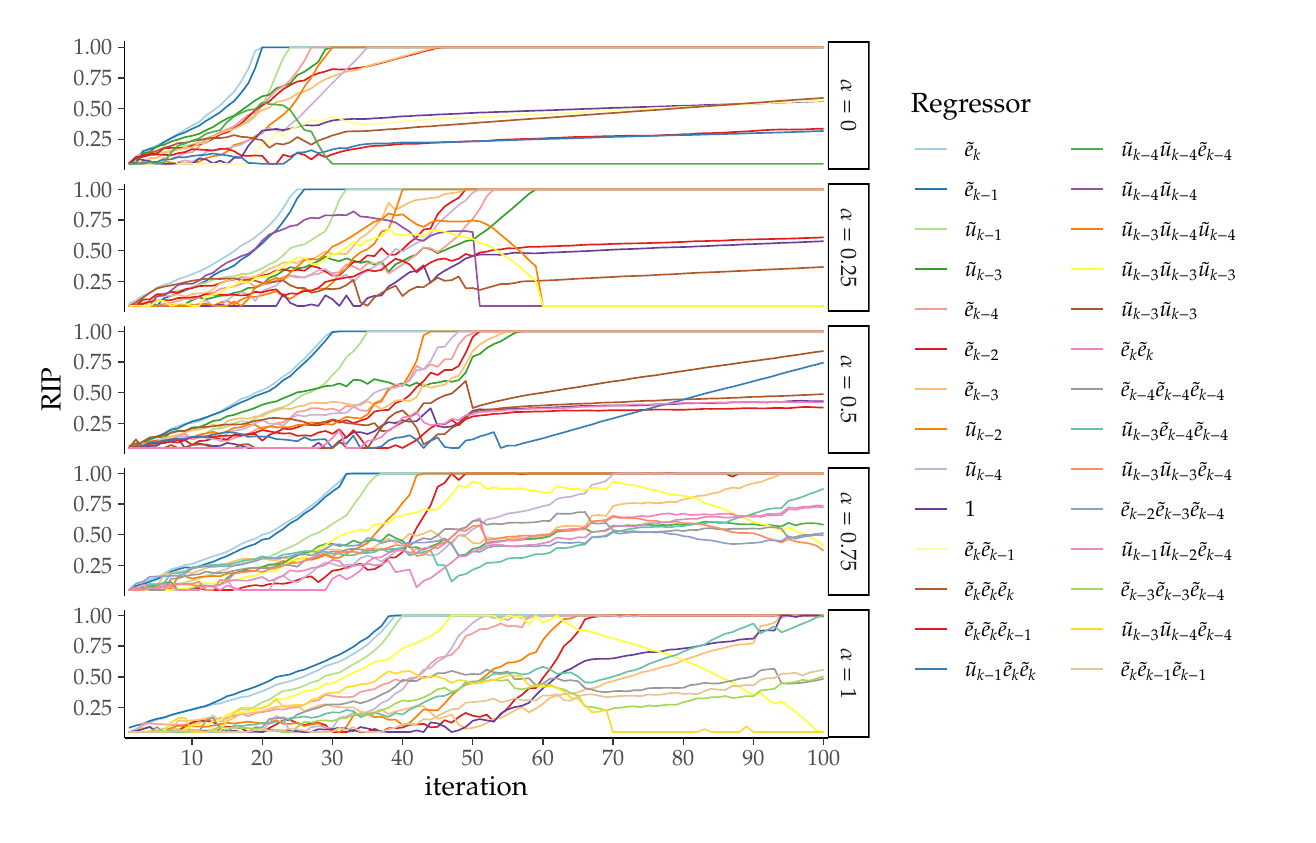
\begin{tikzpicture}[x=1pt,y=1pt]
\definecolor{fillColor}{RGB}{255,255,255}
\path[use as bounding box,fill=fillColor,fill opacity=0.00] (0,0) rectangle (455.24,284.53);
\begin{scope}
\path[clip] (  0.00,  0.00) rectangle (455.24,284.53);
\definecolor{drawColor}{RGB}{255,255,255}
\definecolor{fillColor}{RGB}{255,255,255}

\path[draw=drawColor,line width= 0.5pt,line join=round,line cap=round,fill=fillColor] ( -0.00, -0.00) rectangle (455.24,284.53);
\end{scope}
\begin{scope}
\path[clip] ( 35.05,233.20) rectangle (289.13,279.53);
\definecolor{fillColor}{RGB}{255,255,255}

\path[fill=fillColor] ( 35.05,233.20) rectangle (289.13,279.53);
\definecolor{drawColor}{RGB}{166,206,227}

\path[draw=drawColor,line width= 0.6pt,line join=round] ( 36.57,235.31) --
	( 39.11,238.05) --
	( 41.64,239.55) --
	( 44.18,241.10) --
	( 46.71,241.93) --
	( 49.25,243.41) --
	( 51.79,244.66) --
	( 54.32,246.16) --
	( 56.86,247.71) --
	( 59.39,249.14) --
	( 61.93,250.46) --
	( 64.46,252.75) --
	( 67.00,254.55) --
	( 69.54,256.46) --
	( 72.07,258.99) --
	( 74.61,261.35) --
	( 77.14,265.11) --
	( 79.68,269.52) --
	( 82.21,276.12) --
	( 84.75,277.42) --
	( 87.29,277.42) --
	( 89.82,277.42) --
	( 92.36,277.42) --
	( 94.89,277.42) --
	( 97.43,277.42) --
	( 99.96,277.42) --
	(102.50,277.42) --
	(105.04,277.42) --
	(107.57,277.42) --
	(110.11,277.42) --
	(112.64,277.42) --
	(115.18,277.42) --
	(117.71,277.42) --
	(120.25,277.42) --
	(122.79,277.42) --
	(125.32,277.42) --
	(127.86,277.42) --
	(130.39,277.42) --
	(132.93,277.42) --
	(135.46,277.42) --
	(138.00,277.42) --
	(140.54,277.42) --
	(143.07,277.42) --
	(145.61,277.42) --
	(148.14,277.42) --
	(150.68,277.42) --
	(153.21,277.42) --
	(155.75,277.42) --
	(158.29,277.42) --
	(160.82,277.42) --
	(163.36,277.42) --
	(165.89,277.42) --
	(168.43,277.42) --
	(170.96,277.42) --
	(173.50,277.42) --
	(176.04,277.42) --
	(178.57,277.42) --
	(181.11,277.42) --
	(183.64,277.42) --
	(186.18,277.42) --
	(188.71,277.42) --
	(191.25,277.42) --
	(193.79,277.42) --
	(196.32,277.42) --
	(198.86,277.42) --
	(201.39,277.42) --
	(203.93,277.42) --
	(206.47,277.42) --
	(209.00,277.42) --
	(211.54,277.42) --
	(214.07,277.42) --
	(216.61,277.42) --
	(219.14,277.42) --
	(221.68,277.42) --
	(224.22,277.42) --
	(226.75,277.42) --
	(229.29,277.42) --
	(231.82,277.42) --
	(234.36,277.42) --
	(236.89,277.42) --
	(239.43,277.42) --
	(241.97,277.42) --
	(244.50,277.42) --
	(247.04,277.42) --
	(249.57,277.42) --
	(252.11,277.42) --
	(254.64,277.42) --
	(257.18,277.42) --
	(259.72,277.42) --
	(262.25,277.42) --
	(264.79,277.42) --
	(267.32,277.42) --
	(269.86,277.42) --
	(272.39,277.42) --
	(274.93,277.42) --
	(277.47,277.42) --
	(280.00,277.42) --
	(282.54,277.42) --
	(285.07,277.42) --
	(287.61,277.42);
\definecolor{drawColor}{RGB}{31,120,180}

\path[draw=drawColor,line width= 0.6pt,line join=round] ( 36.57,235.31) --
	( 39.11,235.81) --
	( 41.64,239.93) --
	( 44.18,240.65) --
	( 46.71,241.40) --
	( 49.25,243.11) --
	( 51.79,244.55) --
	( 54.32,245.78) --
	( 56.86,246.67) --
	( 59.39,247.97) --
	( 61.93,249.08) --
	( 64.46,250.86) --
	( 67.00,252.34) --
	( 69.54,253.97) --
	( 72.07,256.13) --
	( 74.61,258.01) --
	( 77.14,260.98) --
	( 79.68,264.37) --
	( 82.21,269.88) --
	( 84.75,277.42) --
	( 87.29,277.42) --
	( 89.82,277.42) --
	( 92.36,277.42) --
	( 94.89,277.42) --
	( 97.43,277.42) --
	( 99.96,277.42) --
	(102.50,277.42) --
	(105.04,277.42) --
	(107.57,277.42) --
	(110.11,277.42) --
	(112.64,277.42) --
	(115.18,277.42) --
	(117.71,277.42) --
	(120.25,277.42) --
	(122.79,277.42) --
	(125.32,277.42) --
	(127.86,277.42) --
	(130.39,277.42) --
	(132.93,277.42) --
	(135.46,277.42) --
	(138.00,277.42) --
	(140.54,277.42) --
	(143.07,277.42) --
	(145.61,277.42) --
	(148.14,277.42) --
	(150.68,277.42) --
	(153.21,277.42) --
	(155.75,277.42) --
	(158.29,277.42) --
	(160.82,277.42) --
	(163.36,277.42) --
	(165.89,277.42) --
	(168.43,277.42) --
	(170.96,277.42) --
	(173.50,277.42) --
	(176.04,277.42) --
	(178.57,277.42) --
	(181.11,277.42) --
	(183.64,277.42) --
	(186.18,277.42) --
	(188.71,277.42) --
	(191.25,277.42) --
	(193.79,277.42) --
	(196.32,277.42) --
	(198.86,277.42) --
	(201.39,277.42) --
	(203.93,277.42) --
	(206.47,277.42) --
	(209.00,277.42) --
	(211.54,277.42) --
	(214.07,277.42) --
	(216.61,277.42) --
	(219.14,277.42) --
	(221.68,277.42) --
	(224.22,277.42) --
	(226.75,277.42) --
	(229.29,277.42) --
	(231.82,277.42) --
	(234.36,277.42) --
	(236.89,277.42) --
	(239.43,277.42) --
	(241.97,277.42) --
	(244.50,277.42) --
	(247.04,277.42) --
	(249.57,277.42) --
	(252.11,277.42) --
	(254.64,277.42) --
	(257.18,277.42) --
	(259.72,277.42) --
	(262.25,277.42) --
	(264.79,277.42) --
	(267.32,277.42) --
	(269.86,277.42) --
	(272.39,277.42) --
	(274.93,277.42) --
	(277.47,277.42) --
	(280.00,277.42) --
	(282.54,277.42) --
	(285.07,277.42) --
	(287.61,277.42);
\definecolor{drawColor}{RGB}{178,223,138}

\path[draw=drawColor,line width= 0.6pt,line join=round] ( 36.57,235.31) --
	( 39.11,237.82) --
	( 41.64,239.03) --
	( 44.18,239.43) --
	( 46.71,239.21) --
	( 49.25,239.51) --
	( 51.79,240.01) --
	( 54.32,240.85) --
	( 56.86,241.85) --
	( 59.39,242.24) --
	( 61.93,243.30) --
	( 64.46,244.55) --
	( 67.00,245.46) --
	( 69.54,246.03) --
	( 72.07,247.57) --
	( 74.61,248.41) --
	( 77.14,249.34) --
	( 79.68,250.36) --
	( 82.21,252.52) --
	( 84.75,256.48) --
	( 87.29,261.45) --
	( 89.82,267.56) --
	( 92.36,273.62) --
	( 94.89,277.42) --
	( 97.43,277.42) --
	( 99.96,277.42) --
	(102.50,277.42) --
	(105.04,277.42) --
	(107.57,277.42) --
	(110.11,277.42) --
	(112.64,277.42) --
	(115.18,277.42) --
	(117.71,277.42) --
	(120.25,277.42) --
	(122.79,277.42) --
	(125.32,277.42) --
	(127.86,277.42) --
	(130.39,277.42) --
	(132.93,277.42) --
	(135.46,277.42) --
	(138.00,277.42) --
	(140.54,277.42) --
	(143.07,277.42) --
	(145.61,277.42) --
	(148.14,277.42) --
	(150.68,277.42) --
	(153.21,277.42) --
	(155.75,277.42) --
	(158.29,277.42) --
	(160.82,277.42) --
	(163.36,277.42) --
	(165.89,277.42) --
	(168.43,277.42) --
	(170.96,277.42) --
	(173.50,277.42) --
	(176.04,277.42) --
	(178.57,277.42) --
	(181.11,277.42) --
	(183.64,277.42) --
	(186.18,277.42) --
	(188.71,277.42) --
	(191.25,277.42) --
	(193.79,277.42) --
	(196.32,277.42) --
	(198.86,277.42) --
	(201.39,277.42) --
	(203.93,277.42) --
	(206.47,277.42) --
	(209.00,277.42) --
	(211.54,277.42) --
	(214.07,277.42) --
	(216.61,277.42) --
	(219.14,277.42) --
	(221.68,277.42) --
	(224.22,277.42) --
	(226.75,277.42) --
	(229.29,277.42) --
	(231.82,277.42) --
	(234.36,277.42) --
	(236.89,277.42) --
	(239.43,277.42) --
	(241.97,277.42) --
	(244.50,277.42) --
	(247.04,277.42) --
	(249.57,277.42) --
	(252.11,277.42) --
	(254.64,277.42) --
	(257.18,277.42) --
	(259.72,277.42) --
	(262.25,277.42) --
	(264.79,277.42) --
	(267.32,277.42) --
	(269.86,277.42) --
	(272.39,277.42) --
	(274.93,277.42) --
	(277.47,277.42) --
	(280.00,277.42) --
	(282.54,277.42) --
	(285.07,277.42) --
	(287.61,277.42);
\definecolor{drawColor}{RGB}{51,160,44}

\path[draw=drawColor,line width= 0.6pt,line join=round] ( 36.57,235.31) --
	( 39.11,235.31) --
	( 41.64,239.18) --
	( 44.18,239.68) --
	( 46.71,241.68) --
	( 49.25,242.18) --
	( 51.79,243.37) --
	( 54.32,244.10) --
	( 56.86,244.98) --
	( 59.39,245.46) --
	( 61.93,246.16) --
	( 64.46,247.49) --
	( 67.00,248.62) --
	( 69.54,250.28) --
	( 72.07,251.71) --
	( 74.61,252.76) --
	( 77.14,254.59) --
	( 79.68,256.39) --
	( 82.21,258.24) --
	( 84.75,259.76) --
	( 87.29,260.26) --
	( 89.82,262.57) --
	( 92.36,263.40) --
	( 94.89,264.38) --
	( 97.43,267.41) --
	( 99.96,268.55) --
	(102.50,270.37) --
	(105.04,272.15) --
	(107.57,276.74) --
	(110.11,277.42) --
	(112.64,277.42) --
	(115.18,277.42) --
	(117.71,277.42) --
	(120.25,277.42) --
	(122.79,277.42) --
	(125.32,277.42) --
	(127.86,277.42) --
	(130.39,277.42) --
	(132.93,277.42) --
	(135.46,277.42) --
	(138.00,277.42) --
	(140.54,277.42) --
	(143.07,277.42) --
	(145.61,277.42) --
	(148.14,277.42) --
	(150.68,277.42) --
	(153.21,277.42) --
	(155.75,277.42) --
	(158.29,277.42) --
	(160.82,277.42) --
	(163.36,277.42) --
	(165.89,277.42) --
	(168.43,277.42) --
	(170.96,277.42) --
	(173.50,277.42) --
	(176.04,277.42) --
	(178.57,277.42) --
	(181.11,277.42) --
	(183.64,277.42) --
	(186.18,277.42) --
	(188.71,277.42) --
	(191.25,277.42) --
	(193.79,277.42) --
	(196.32,277.42) --
	(198.86,277.42) --
	(201.39,277.42) --
	(203.93,277.42) --
	(206.47,277.42) --
	(209.00,277.42) --
	(211.54,277.42) --
	(214.07,277.42) --
	(216.61,277.42) --
	(219.14,277.42) --
	(221.68,277.42) --
	(224.22,277.42) --
	(226.75,277.42) --
	(229.29,277.42) --
	(231.82,277.42) --
	(234.36,277.42) --
	(236.89,277.42) --
	(239.43,277.42) --
	(241.97,277.42) --
	(244.50,277.42) --
	(247.04,277.42) --
	(249.57,277.42) --
	(252.11,277.42) --
	(254.64,277.42) --
	(257.18,277.42) --
	(259.72,277.42) --
	(262.25,277.42) --
	(264.79,277.42) --
	(267.32,277.42) --
	(269.86,277.42) --
	(272.39,277.42) --
	(274.93,277.42) --
	(277.47,277.42) --
	(280.00,277.42) --
	(282.54,277.42) --
	(285.07,277.42) --
	(287.61,277.42);
\definecolor{drawColor}{RGB}{251,154,153}

\path[draw=drawColor,line width= 0.6pt,line join=round] ( 36.57,235.31) --
	( 39.11,235.31) --
	( 41.64,235.31) --
	( 44.18,235.31) --
	( 46.71,236.05) --
	( 49.25,237.34) --
	( 51.79,237.24) --
	( 54.32,238.06) --
	( 56.86,239.32) --
	( 59.39,239.45) --
	( 61.93,241.60) --
	( 64.46,244.36) --
	( 67.00,245.41) --
	( 69.54,246.81) --
	( 72.07,247.81) --
	( 74.61,248.87) --
	( 77.14,251.02) --
	( 79.68,253.04) --
	( 82.21,253.72) --
	( 84.75,256.30) --
	( 87.29,259.33) --
	( 89.82,261.89) --
	( 92.36,263.32) --
	( 94.89,265.54) --
	( 97.43,268.78) --
	( 99.96,272.49) --
	(102.50,277.42) --
	(105.04,277.42) --
	(107.57,277.42) --
	(110.11,277.42) --
	(112.64,277.42) --
	(115.18,277.42) --
	(117.71,277.42) --
	(120.25,277.42) --
	(122.79,277.42) --
	(125.32,277.42) --
	(127.86,277.42) --
	(130.39,277.42) --
	(132.93,277.42) --
	(135.46,277.42) --
	(138.00,277.42) --
	(140.54,277.42) --
	(143.07,277.42) --
	(145.61,277.42) --
	(148.14,277.42) --
	(150.68,277.42) --
	(153.21,277.42) --
	(155.75,277.42) --
	(158.29,277.42) --
	(160.82,277.42) --
	(163.36,277.42) --
	(165.89,277.42) --
	(168.43,277.42) --
	(170.96,277.42) --
	(173.50,277.42) --
	(176.04,277.42) --
	(178.57,277.42) --
	(181.11,277.42) --
	(183.64,277.42) --
	(186.18,277.42) --
	(188.71,277.42) --
	(191.25,277.42) --
	(193.79,277.42) --
	(196.32,277.42) --
	(198.86,277.42) --
	(201.39,277.42) --
	(203.93,277.42) --
	(206.47,277.42) --
	(209.00,277.42) --
	(211.54,277.42) --
	(214.07,277.42) --
	(216.61,277.42) --
	(219.14,277.42) --
	(221.68,277.42) --
	(224.22,277.42) --
	(226.75,277.42) --
	(229.29,277.42) --
	(231.82,277.42) --
	(234.36,277.42) --
	(236.89,277.42) --
	(239.43,277.42) --
	(241.97,277.42) --
	(244.50,277.42) --
	(247.04,277.42) --
	(249.57,277.42) --
	(252.11,277.42) --
	(254.64,277.42) --
	(257.18,277.42) --
	(259.72,277.42) --
	(262.25,277.42) --
	(264.79,277.42) --
	(267.32,277.42) --
	(269.86,277.42) --
	(272.39,277.42) --
	(274.93,277.42) --
	(277.47,277.42) --
	(280.00,277.42) --
	(282.54,277.42) --
	(285.07,277.42) --
	(287.61,277.42);
\definecolor{drawColor}{RGB}{227,26,28}

\path[draw=drawColor,line width= 0.6pt,line join=round] ( 36.57,235.31) --
	( 39.11,237.40) --
	( 41.64,238.56) --
	( 44.18,238.90) --
	( 46.71,239.11) --
	( 49.25,240.93) --
	( 51.79,241.10) --
	( 54.32,241.14) --
	( 56.86,240.90) --
	( 59.39,241.95) --
	( 61.93,242.31) --
	( 64.46,243.04) --
	( 67.00,244.43) --
	( 69.54,245.97) --
	( 72.07,246.72) --
	( 74.61,248.14) --
	( 77.14,249.82) --
	( 79.68,252.29) --
	( 82.21,254.74) --
	( 84.75,256.55) --
	( 87.29,257.84) --
	( 89.82,260.20) --
	( 92.36,262.29) --
	( 94.89,263.81) --
	( 97.43,265.06) --
	( 99.96,265.46) --
	(102.50,267.06) --
	(105.04,268.06) --
	(107.57,268.69) --
	(110.11,269.56) --
	(112.64,269.42) --
	(115.18,269.46) --
	(117.71,269.81) --
	(120.25,270.10) --
	(122.79,270.50) --
	(125.32,271.19) --
	(127.86,271.78) --
	(130.39,272.46) --
	(132.93,273.18) --
	(135.46,273.89) --
	(138.00,274.53) --
	(140.54,275.19) --
	(143.07,275.97) --
	(145.61,276.54) --
	(148.14,277.25) --
	(150.68,277.42) --
	(153.21,277.42) --
	(155.75,277.42) --
	(158.29,277.42) --
	(160.82,277.42) --
	(163.36,277.42) --
	(165.89,277.42) --
	(168.43,277.42) --
	(170.96,277.42) --
	(173.50,277.42) --
	(176.04,277.42) --
	(178.57,277.42) --
	(181.11,277.42) --
	(183.64,277.42) --
	(186.18,277.42) --
	(188.71,277.42) --
	(191.25,277.42) --
	(193.79,277.42) --
	(196.32,277.42) --
	(198.86,277.42) --
	(201.39,277.42) --
	(203.93,277.42) --
	(206.47,277.42) --
	(209.00,277.42) --
	(211.54,277.42) --
	(214.07,277.42) --
	(216.61,277.42) --
	(219.14,277.42) --
	(221.68,277.42) --
	(224.22,277.42) --
	(226.75,277.42) --
	(229.29,277.42) --
	(231.82,277.42) --
	(234.36,277.42) --
	(236.89,277.42) --
	(239.43,277.42) --
	(241.97,277.42) --
	(244.50,277.42) --
	(247.04,277.42) --
	(249.57,277.42) --
	(252.11,277.42) --
	(254.64,277.42) --
	(257.18,277.42) --
	(259.72,277.42) --
	(262.25,277.42) --
	(264.79,277.42) --
	(267.32,277.42) --
	(269.86,277.42) --
	(272.39,277.42) --
	(274.93,277.42) --
	(277.47,277.42) --
	(280.00,277.42) --
	(282.54,277.42) --
	(285.07,277.42) --
	(287.61,277.42);
\definecolor{drawColor}{RGB}{253,191,111}

\path[draw=drawColor,line width= 0.6pt,line join=round] ( 36.57,235.31) --
	( 39.11,235.31) --
	( 41.64,235.56) --
	( 44.18,237.41) --
	( 46.71,237.46) --
	( 49.25,239.01) --
	( 51.79,239.88) --
	( 54.32,240.39) --
	( 56.86,241.10) --
	( 59.39,241.30) --
	( 61.93,242.66) --
	( 64.46,242.92) --
	( 67.00,245.14) --
	( 69.54,246.36) --
	( 72.07,247.26) --
	( 74.61,247.89) --
	( 77.14,249.25) --
	( 79.68,251.02) --
	( 82.21,252.99) --
	( 84.75,254.79) --
	( 87.29,255.62) --
	( 89.82,257.63) --
	( 92.36,258.15) --
	( 94.89,259.05) --
	( 97.43,260.77) --
	( 99.96,261.43) --
	(102.50,262.60) --
	(105.04,264.49) --
	(107.57,265.86) --
	(110.11,266.95) --
	(112.64,267.79) --
	(115.18,268.64) --
	(117.71,269.07) --
	(120.25,269.66) --
	(122.79,270.63) --
	(125.32,271.37) --
	(127.86,272.02) --
	(130.39,272.65) --
	(132.93,273.34) --
	(135.46,274.14) --
	(138.00,274.84) --
	(140.54,275.55) --
	(143.07,276.23) --
	(145.61,276.95) --
	(148.14,277.42) --
	(150.68,277.42) --
	(153.21,277.42) --
	(155.75,277.42) --
	(158.29,277.42) --
	(160.82,277.42) --
	(163.36,277.42) --
	(165.89,277.42) --
	(168.43,277.42) --
	(170.96,277.42) --
	(173.50,277.42) --
	(176.04,277.42) --
	(178.57,277.42) --
	(181.11,277.42) --
	(183.64,277.42) --
	(186.18,277.42) --
	(188.71,277.42) --
	(191.25,277.42) --
	(193.79,277.42) --
	(196.32,277.42) --
	(198.86,277.42) --
	(201.39,277.42) --
	(203.93,277.42) --
	(206.47,277.42) --
	(209.00,277.42) --
	(211.54,277.42) --
	(214.07,277.42) --
	(216.61,277.42) --
	(219.14,277.42) --
	(221.68,277.42) --
	(224.22,277.42) --
	(226.75,277.42) --
	(229.29,277.42) --
	(231.82,277.42) --
	(234.36,277.42) --
	(236.89,277.42) --
	(239.43,277.42) --
	(241.97,277.42) --
	(244.50,277.42) --
	(247.04,277.42) --
	(249.57,277.42) --
	(252.11,277.42) --
	(254.64,277.42) --
	(257.18,277.42) --
	(259.72,277.42) --
	(262.25,277.42) --
	(264.79,277.42) --
	(267.32,277.42) --
	(269.86,277.42) --
	(272.39,277.42) --
	(274.93,277.42) --
	(277.47,277.42) --
	(280.00,277.42) --
	(282.54,277.42) --
	(285.07,277.42) --
	(287.61,277.42);
\definecolor{drawColor}{RGB}{255,127,0}

\path[draw=drawColor,line width= 0.6pt,line join=round] ( 36.57,235.31) --
	( 39.11,235.31) --
	( 41.64,236.01) --
	( 44.18,235.31) --
	( 46.71,236.24) --
	( 49.25,236.32) --
	( 51.79,235.75) --
	( 54.32,235.31) --
	( 56.86,235.51) --
	( 59.39,235.61) --
	( 61.93,236.11) --
	( 64.46,237.37) --
	( 67.00,238.11) --
	( 69.54,238.40) --
	( 72.07,239.79) --
	( 74.61,242.15) --
	( 77.14,242.78) --
	( 79.68,243.78) --
	( 82.21,245.29) --
	( 84.75,246.36) --
	( 87.29,249.28) --
	( 89.82,251.15) --
	( 92.36,253.12) --
	( 94.89,255.45) --
	( 97.43,258.88) --
	( 99.96,263.11) --
	(102.50,266.52) --
	(105.04,270.83) --
	(107.57,274.11) --
	(110.11,277.42) --
	(112.64,277.42) --
	(115.18,277.42) --
	(117.71,277.42) --
	(120.25,277.42) --
	(122.79,277.42) --
	(125.32,277.42) --
	(127.86,277.42) --
	(130.39,277.42) --
	(132.93,277.42) --
	(135.46,277.42) --
	(138.00,277.42) --
	(140.54,277.42) --
	(143.07,277.42) --
	(145.61,277.42) --
	(148.14,277.42) --
	(150.68,277.42) --
	(153.21,277.42) --
	(155.75,277.42) --
	(158.29,277.42) --
	(160.82,277.42) --
	(163.36,277.42) --
	(165.89,277.42) --
	(168.43,277.42) --
	(170.96,277.42) --
	(173.50,277.42) --
	(176.04,277.42) --
	(178.57,277.42) --
	(181.11,277.42) --
	(183.64,277.42) --
	(186.18,277.42) --
	(188.71,277.42) --
	(191.25,277.42) --
	(193.79,277.42) --
	(196.32,277.42) --
	(198.86,277.42) --
	(201.39,277.42) --
	(203.93,277.42) --
	(206.47,277.42) --
	(209.00,277.42) --
	(211.54,277.42) --
	(214.07,277.42) --
	(216.61,277.42) --
	(219.14,277.42) --
	(221.68,277.42) --
	(224.22,277.42) --
	(226.75,277.42) --
	(229.29,277.42) --
	(231.82,277.42) --
	(234.36,277.42) --
	(236.89,277.42) --
	(239.43,277.42) --
	(241.97,277.42) --
	(244.50,277.42) --
	(247.04,277.42) --
	(249.57,277.42) --
	(252.11,277.42) --
	(254.64,277.42) --
	(257.18,277.42) --
	(259.72,277.42) --
	(262.25,277.42) --
	(264.79,277.42) --
	(267.32,277.42) --
	(269.86,277.42) --
	(272.39,277.42) --
	(274.93,277.42) --
	(277.47,277.42) --
	(280.00,277.42) --
	(282.54,277.42) --
	(285.07,277.42) --
	(287.61,277.42);
\definecolor{drawColor}{RGB}{202,178,214}

\path[draw=drawColor,line width= 0.6pt,line join=round] ( 36.57,235.31) --
	( 39.11,235.31) --
	( 41.64,235.31) --
	( 44.18,235.49) --
	( 46.71,235.31) --
	( 49.25,235.31) --
	( 51.79,235.31) --
	( 54.32,235.95) --
	( 56.86,236.60) --
	( 59.39,236.11) --
	( 61.93,237.34) --
	( 64.46,239.66) --
	( 67.00,240.13) --
	( 69.54,240.46) --
	( 72.07,240.91) --
	( 74.61,241.67) --
	( 77.14,242.24) --
	( 79.68,243.89) --
	( 82.21,244.51) --
	( 84.75,246.67) --
	( 87.29,248.31) --
	( 89.82,247.36) --
	( 92.36,247.13) --
	( 94.89,249.52) --
	( 97.43,251.52) --
	( 99.96,254.14) --
	(102.50,256.67) --
	(105.04,259.24) --
	(107.57,261.92) --
	(110.11,264.50) --
	(112.64,267.00) --
	(115.18,269.50) --
	(117.71,271.95) --
	(120.25,274.55) --
	(122.79,277.42) --
	(125.32,277.42) --
	(127.86,277.42) --
	(130.39,277.42) --
	(132.93,277.42) --
	(135.46,277.42) --
	(138.00,277.42) --
	(140.54,277.42) --
	(143.07,277.42) --
	(145.61,277.42) --
	(148.14,277.42) --
	(150.68,277.42) --
	(153.21,277.42) --
	(155.75,277.42) --
	(158.29,277.42) --
	(160.82,277.42) --
	(163.36,277.42) --
	(165.89,277.42) --
	(168.43,277.42) --
	(170.96,277.42) --
	(173.50,277.42) --
	(176.04,277.42) --
	(178.57,277.42) --
	(181.11,277.42) --
	(183.64,277.42) --
	(186.18,277.42) --
	(188.71,277.42) --
	(191.25,277.42) --
	(193.79,277.42) --
	(196.32,277.42) --
	(198.86,277.42) --
	(201.39,277.42) --
	(203.93,277.42) --
	(206.47,277.42) --
	(209.00,277.42) --
	(211.54,277.42) --
	(214.07,277.42) --
	(216.61,277.42) --
	(219.14,277.42) --
	(221.68,277.42) --
	(224.22,277.42) --
	(226.75,277.42) --
	(229.29,277.42) --
	(231.82,277.42) --
	(234.36,277.42) --
	(236.89,277.42) --
	(239.43,277.42) --
	(241.97,277.42) --
	(244.50,277.42) --
	(247.04,277.42) --
	(249.57,277.42) --
	(252.11,277.42) --
	(254.64,277.42) --
	(257.18,277.42) --
	(259.72,277.42) --
	(262.25,277.42) --
	(264.79,277.42) --
	(267.32,277.42) --
	(269.86,277.42) --
	(272.39,277.42) --
	(274.93,277.42) --
	(277.47,277.42) --
	(280.00,277.42) --
	(282.54,277.42) --
	(285.07,277.42) --
	(287.61,277.42);
\definecolor{drawColor}{RGB}{106,61,154}

\path[draw=drawColor,line width= 0.6pt,line join=round] ( 36.57,235.31) --
	( 39.11,237.22) --
	( 41.64,236.73) --
	( 44.18,236.27) --
	( 46.71,235.59) --
	( 49.25,235.31) --
	( 51.79,235.31) --
	( 54.32,235.59) --
	( 56.86,235.31) --
	( 59.39,235.31) --
	( 61.93,237.20) --
	( 64.46,236.93) --
	( 67.00,235.45) --
	( 69.54,236.51) --
	( 72.07,235.31) --
	( 74.61,237.50) --
	( 77.14,237.56) --
	( 79.68,241.76) --
	( 82.21,244.65) --
	( 84.75,247.35) --
	( 87.29,247.57) --
	( 89.82,247.95) --
	( 92.36,247.52) --
	( 94.89,247.98) --
	( 97.43,248.72) --
	( 99.96,249.35) --
	(102.50,249.17) --
	(105.04,249.29) --
	(107.57,250.27) --
	(110.11,250.98) --
	(112.64,251.31) --
	(115.18,251.43) --
	(117.71,251.58) --
	(120.25,251.51) --
	(122.79,251.56) --
	(125.32,251.78) --
	(127.86,251.90) --
	(130.39,252.05) --
	(132.93,252.31) --
	(135.46,252.48) --
	(138.00,252.58) --
	(140.54,252.76) --
	(143.07,252.87) --
	(145.61,252.97) --
	(148.14,253.16) --
	(150.68,253.23) --
	(153.21,253.35) --
	(155.75,253.45) --
	(158.29,253.60) --
	(160.82,253.72) --
	(163.36,253.85) --
	(165.89,253.91) --
	(168.43,254.02) --
	(170.96,254.12) --
	(173.50,254.17) --
	(176.04,254.28) --
	(178.57,254.36) --
	(181.11,254.45) --
	(183.64,254.55) --
	(186.18,254.62) --
	(188.71,254.69) --
	(191.25,254.78) --
	(193.79,254.90) --
	(196.32,254.97) --
	(198.86,255.08) --
	(201.39,255.18) --
	(203.93,255.25) --
	(206.47,255.34) --
	(209.00,255.44) --
	(211.54,255.54) --
	(214.07,255.61) --
	(216.61,255.69) --
	(219.14,255.76) --
	(221.68,255.84) --
	(224.22,255.91) --
	(226.75,255.99) --
	(229.29,256.04) --
	(231.82,256.16) --
	(234.36,256.24) --
	(236.89,256.30) --
	(239.43,256.36) --
	(241.97,256.44) --
	(244.50,256.56) --
	(247.04,256.64) --
	(249.57,256.71) --
	(252.11,256.77) --
	(254.64,256.87) --
	(257.18,256.92) --
	(259.72,257.00) --
	(262.25,257.08) --
	(264.79,257.15) --
	(267.32,257.27) --
	(269.86,257.37) --
	(272.39,257.46) --
	(274.93,257.56) --
	(277.47,257.64) --
	(280.00,257.71) --
	(282.54,257.81) --
	(285.07,257.91) --
	(287.61,258.00);
\definecolor{drawColor}{RGB}{255,255,153}

\path[draw=drawColor,line width= 0.6pt,line join=round] ( 36.57,235.31) --
	( 39.11,235.31) --
	( 41.64,235.31) --
	( 44.18,235.31) --
	( 46.71,236.54) --
	( 49.25,236.31) --
	( 51.79,237.59) --
	( 54.32,235.31) --
	( 56.86,235.31) --
	( 59.39,235.31) --
	( 61.93,235.31) --
	( 64.46,235.31) --
	( 67.00,235.31) --
	( 69.54,235.31) --
	( 72.07,235.31) --
	( 74.61,235.31) --
	( 77.14,235.31) --
	( 79.68,235.31) --
	( 82.21,238.96) --
	( 84.75,242.44) --
	( 87.29,243.39) --
	( 89.82,246.84) --
	( 92.36,245.41) --
	( 94.89,247.65) --
	( 97.43,248.87) --
	( 99.96,249.60) --
	(102.50,251.13) --
	(105.04,250.65) --
	(107.57,251.30) --
	(110.11,252.26) --
	(112.64,251.78) --
	(115.18,250.43) --
	(117.71,250.17) --
	(120.25,249.71) --
	(122.79,249.75) --
	(125.32,249.79) --
	(127.86,249.82) --
	(130.39,250.12) --
	(132.93,250.32) --
	(135.46,250.61) --
	(138.00,250.82) --
	(140.54,251.02) --
	(143.07,251.18) --
	(145.61,251.42) --
	(148.14,251.55) --
	(150.68,251.67) --
	(153.21,251.81) --
	(155.75,251.90) --
	(158.29,251.93) --
	(160.82,252.05) --
	(163.36,252.26) --
	(165.89,252.38) --
	(168.43,252.45) --
	(170.96,252.58) --
	(173.50,252.69) --
	(176.04,252.87) --
	(178.57,252.97) --
	(181.11,253.07) --
	(183.64,253.15) --
	(186.18,253.23) --
	(188.71,253.31) --
	(191.25,253.39) --
	(193.79,253.60) --
	(196.32,253.71) --
	(198.86,253.99) --
	(201.39,254.15) --
	(203.93,254.34) --
	(206.47,254.43) --
	(209.00,254.61) --
	(211.54,254.73) --
	(214.07,254.77) --
	(216.61,254.86) --
	(219.14,255.01) --
	(221.68,255.11) --
	(224.22,255.35) --
	(226.75,255.45) --
	(229.29,255.53) --
	(231.82,255.64) --
	(234.36,255.75) --
	(236.89,255.86) --
	(239.43,255.94) --
	(241.97,256.05) --
	(244.50,256.13) --
	(247.04,256.31) --
	(249.57,256.41) --
	(252.11,256.57) --
	(254.64,256.69) --
	(257.18,256.75) --
	(259.72,256.80) --
	(262.25,257.03) --
	(264.79,257.19) --
	(267.32,257.26) --
	(269.86,257.42) --
	(272.39,257.56) --
	(274.93,257.63) --
	(277.47,257.79) --
	(280.00,257.83) --
	(282.54,257.93) --
	(285.07,258.04) --
	(287.61,258.15);
\definecolor{drawColor}{RGB}{177,89,40}

\path[draw=drawColor,line width= 0.6pt,line join=round] ( 36.57,235.70) --
	( 39.11,237.01) --
	( 41.64,237.98) --
	( 44.18,239.31) --
	( 46.71,240.06) --
	( 49.25,241.10) --
	( 51.79,241.81) --
	( 54.32,242.78) --
	( 56.86,242.97) --
	( 59.39,243.51) --
	( 61.93,243.96) --
	( 64.46,244.37) --
	( 67.00,244.71) --
	( 69.54,244.64) --
	( 72.07,244.96) --
	( 74.61,245.72) --
	( 77.14,245.09) --
	( 79.68,244.89) --
	( 82.21,244.33) --
	( 84.75,243.90) --
	( 87.29,241.11) --
	( 89.82,242.72) --
	( 92.36,242.31) --
	( 94.89,243.13) --
	( 97.43,245.00) --
	( 99.96,243.60) --
	(102.50,242.24) --
	(105.04,243.72) --
	(107.57,244.63) --
	(110.11,245.59) --
	(112.64,246.27) --
	(115.18,247.02) --
	(117.71,247.08) --
	(120.25,247.10) --
	(122.79,247.21) --
	(125.32,247.42) --
	(127.86,247.59) --
	(130.39,247.81) --
	(132.93,247.92) --
	(135.46,248.13) --
	(138.00,248.34) --
	(140.54,248.59) --
	(143.07,248.76) --
	(145.61,248.87) --
	(148.14,249.11) --
	(150.68,249.28) --
	(153.21,249.45) --
	(155.75,249.65) --
	(158.29,249.84) --
	(160.82,250.03) --
	(163.36,250.25) --
	(165.89,250.41) --
	(168.43,250.59) --
	(170.96,250.80) --
	(173.50,250.97) --
	(176.04,251.17) --
	(178.57,251.35) --
	(181.11,251.53) --
	(183.64,251.70) --
	(186.18,251.85) --
	(188.71,252.02) --
	(191.25,252.22) --
	(193.79,252.42) --
	(196.32,252.60) --
	(198.86,252.78) --
	(201.39,252.97) --
	(203.93,253.15) --
	(206.47,253.35) --
	(209.00,253.53) --
	(211.54,253.69) --
	(214.07,253.87) --
	(216.61,254.07) --
	(219.14,254.25) --
	(221.68,254.43) --
	(224.22,254.61) --
	(226.75,254.78) --
	(229.29,254.95) --
	(231.82,255.16) --
	(234.36,255.35) --
	(236.89,255.55) --
	(239.43,255.73) --
	(241.97,255.89) --
	(244.50,256.08) --
	(247.04,256.27) --
	(249.57,256.43) --
	(252.11,256.61) --
	(254.64,256.79) --
	(257.18,256.98) --
	(259.72,257.16) --
	(262.25,257.34) --
	(264.79,257.52) --
	(267.32,257.71) --
	(269.86,257.90) --
	(272.39,258.09) --
	(274.93,258.29) --
	(277.47,258.47) --
	(280.00,258.63) --
	(282.54,258.80) --
	(285.07,258.96) --
	(287.61,259.16);
\definecolor{drawColor}{RGB}{228,26,28}

\path[draw=drawColor,line width= 0.6pt,line join=round] ( 36.57,235.31) --
	( 39.11,237.78) --
	( 41.64,237.86) --
	( 44.18,238.54) --
	( 46.71,238.69) --
	( 49.25,238.61) --
	( 51.79,238.42) --
	( 54.32,239.16) --
	( 56.86,239.59) --
	( 59.39,240.62) --
	( 61.93,240.49) --
	( 64.46,240.34) --
	( 67.00,240.17) --
	( 69.54,240.74) --
	( 72.07,240.72) --
	( 74.61,239.87) --
	( 77.14,238.36) --
	( 79.68,238.18) --
	( 82.21,238.33) --
	( 84.75,238.23) --
	( 87.29,235.31) --
	( 89.82,235.31) --
	( 92.36,238.59) --
	( 94.89,237.89) --
	( 97.43,239.25) --
	( 99.96,238.59) --
	(102.50,236.93) --
	(105.04,238.86) --
	(107.57,237.75) --
	(110.11,238.76) --
	(112.64,239.54) --
	(115.18,240.20) --
	(117.71,240.63) --
	(120.25,241.03) --
	(122.79,241.54) --
	(125.32,241.80) --
	(127.86,241.89) --
	(130.39,242.08) --
	(132.93,242.33) --
	(135.46,242.52) --
	(138.00,242.57) --
	(140.54,242.57) --
	(143.07,242.74) --
	(145.61,242.89) --
	(148.14,243.05) --
	(150.68,243.11) --
	(153.21,243.17) --
	(155.75,243.28) --
	(158.29,243.41) --
	(160.82,243.46) --
	(163.36,243.49) --
	(165.89,243.59) --
	(168.43,243.83) --
	(170.96,244.03) --
	(173.50,244.11) --
	(176.04,244.19) --
	(178.57,244.29) --
	(181.11,244.31) --
	(183.64,244.41) --
	(186.18,244.51) --
	(188.71,244.65) --
	(191.25,244.73) --
	(193.79,244.83) --
	(196.32,244.96) --
	(198.86,245.06) --
	(201.39,245.08) --
	(203.93,245.15) --
	(206.47,245.22) --
	(209.00,245.33) --
	(211.54,245.34) --
	(214.07,245.39) --
	(216.61,245.49) --
	(219.14,245.49) --
	(221.68,245.44) --
	(224.22,245.47) --
	(226.75,245.54) --
	(229.29,245.67) --
	(231.82,245.76) --
	(234.36,245.85) --
	(236.89,246.01) --
	(239.43,246.06) --
	(241.97,246.26) --
	(244.50,246.40) --
	(247.04,246.42) --
	(249.57,246.51) --
	(252.11,246.62) --
	(254.64,246.80) --
	(257.18,246.90) --
	(259.72,247.05) --
	(262.25,247.21) --
	(264.79,247.40) --
	(267.32,247.55) --
	(269.86,247.67) --
	(272.39,247.75) --
	(274.93,247.69) --
	(277.47,247.74) --
	(280.00,247.75) --
	(282.54,247.85) --
	(285.07,248.00) --
	(287.61,247.99);
\definecolor{drawColor}{RGB}{55,126,184}

\path[draw=drawColor,line width= 0.6pt,line join=round] ( 36.57,235.31) --
	( 39.11,235.31) --
	( 41.64,235.54) --
	( 44.18,235.91) --
	( 46.71,236.05) --
	( 49.25,236.87) --
	( 51.79,236.94) --
	( 54.32,237.71) --
	( 56.86,237.69) --
	( 59.39,238.16) --
	( 61.93,238.44) --
	( 64.46,238.61) --
	( 67.00,239.06) --
	( 69.54,238.70) --
	( 72.07,238.38) --
	( 74.61,237.86) --
	( 77.14,237.70) --
	( 79.68,235.66) --
	( 82.21,235.55) --
	( 84.75,235.31) --
	( 87.29,235.31) --
	( 89.82,235.31) --
	( 92.36,235.31) --
	( 94.89,237.08) --
	( 97.43,239.45) --
	( 99.96,239.49) --
	(102.50,240.23) --
	(105.04,239.21) --
	(107.57,239.75) --
	(110.11,240.52) --
	(112.64,241.04) --
	(115.18,240.92) --
	(117.71,241.64) --
	(120.25,242.23) --
	(122.79,242.50) --
	(125.32,242.68) --
	(127.86,242.70) --
	(130.39,242.67) --
	(132.93,242.91) --
	(135.46,243.04) --
	(138.00,243.03) --
	(140.54,243.06) --
	(143.07,243.09) --
	(145.61,243.07) --
	(148.14,243.04) --
	(150.68,243.14) --
	(153.21,243.20) --
	(155.75,243.28) --
	(158.29,243.37) --
	(160.82,243.45) --
	(163.36,243.55) --
	(165.89,243.61) --
	(168.43,243.68) --
	(170.96,243.75) --
	(173.50,243.84) --
	(176.04,243.93) --
	(178.57,244.03) --
	(181.11,244.11) --
	(183.64,244.19) --
	(186.18,244.25) --
	(188.71,244.33) --
	(191.25,244.40) --
	(193.79,244.45) --
	(196.32,244.56) --
	(198.86,244.65) --
	(201.39,244.70) --
	(203.93,244.79) --
	(206.47,244.88) --
	(209.00,244.96) --
	(211.54,245.05) --
	(214.07,245.08) --
	(216.61,245.16) --
	(219.14,245.24) --
	(221.68,245.29) --
	(224.22,245.39) --
	(226.75,245.46) --
	(229.29,245.54) --
	(231.82,245.63) --
	(234.36,245.68) --
	(236.89,245.72) --
	(239.43,245.76) --
	(241.97,245.82) --
	(244.50,245.92) --
	(247.04,245.98) --
	(249.57,246.03) --
	(252.11,246.10) --
	(254.64,246.20) --
	(257.18,246.23) --
	(259.72,246.32) --
	(262.25,246.41) --
	(264.79,246.48) --
	(267.32,246.53) --
	(269.86,246.60) --
	(272.39,246.68) --
	(274.93,246.76) --
	(277.47,246.85) --
	(280.00,246.91) --
	(282.54,247.03) --
	(285.07,247.13) --
	(287.61,247.19);
\definecolor{drawColor}{RGB}{77,175,74}

\path[draw=drawColor,line width= 0.6pt,line join=round] ( 36.57,235.31) --
	( 39.11,235.31) --
	( 41.64,235.31) --
	( 44.18,235.82) --
	( 46.71,235.31) --
	( 49.25,235.85) --
	( 51.79,239.30) --
	( 54.32,241.93) --
	( 56.86,242.65) --
	( 59.39,243.70) --
	( 61.93,244.46) --
	( 64.46,246.21) --
	( 67.00,246.89) --
	( 69.54,247.50) --
	( 72.07,250.44) --
	( 74.61,252.46) --
	( 77.14,253.73) --
	( 79.68,254.77) --
	( 82.21,255.09) --
	( 84.75,257.48) --
	( 87.29,256.92) --
	( 89.82,256.73) --
	( 92.36,256.47) --
	( 94.89,254.74) --
	( 97.43,251.03) --
	( 99.96,247.58) --
	(102.50,246.98) --
	(105.04,242.14) --
	(107.57,238.00) --
	(110.11,235.31) --
	(112.64,235.31) --
	(115.18,235.31) --
	(117.71,235.31) --
	(120.25,235.31) --
	(122.79,235.31) --
	(125.32,235.31) --
	(127.86,235.31) --
	(130.39,235.31) --
	(132.93,235.31) --
	(135.46,235.31) --
	(138.00,235.31) --
	(140.54,235.31) --
	(143.07,235.31) --
	(145.61,235.31) --
	(148.14,235.31) --
	(150.68,235.31) --
	(153.21,235.31) --
	(155.75,235.31) --
	(158.29,235.31) --
	(160.82,235.31) --
	(163.36,235.31) --
	(165.89,235.31) --
	(168.43,235.31) --
	(170.96,235.31) --
	(173.50,235.31) --
	(176.04,235.31) --
	(178.57,235.31) --
	(181.11,235.31) --
	(183.64,235.31) --
	(186.18,235.31) --
	(188.71,235.31) --
	(191.25,235.31) --
	(193.79,235.31) --
	(196.32,235.31) --
	(198.86,235.31) --
	(201.39,235.31) --
	(203.93,235.31) --
	(206.47,235.31) --
	(209.00,235.31) --
	(211.54,235.31) --
	(214.07,235.31) --
	(216.61,235.31) --
	(219.14,235.31) --
	(221.68,235.31) --
	(224.22,235.31) --
	(226.75,235.31) --
	(229.29,235.31) --
	(231.82,235.31) --
	(234.36,235.31) --
	(236.89,235.31) --
	(239.43,235.31) --
	(241.97,235.31) --
	(244.50,235.31) --
	(247.04,235.31) --
	(249.57,235.31) --
	(252.11,235.31) --
	(254.64,235.31) --
	(257.18,235.31) --
	(259.72,235.31) --
	(262.25,235.31) --
	(264.79,235.31) --
	(267.32,235.31) --
	(269.86,235.31) --
	(272.39,235.31) --
	(274.93,235.31) --
	(277.47,235.31) --
	(280.00,235.31) --
	(282.54,235.31) --
	(285.07,235.31) --
	(287.61,235.31);
\end{scope}
\begin{scope}
\path[clip] ( 35.05,181.87) rectangle (289.13,228.20);
\definecolor{fillColor}{RGB}{255,255,255}

\path[fill=fillColor] ( 35.05,181.87) rectangle (289.13,228.20);
\definecolor{drawColor}{RGB}{166,206,227}

\path[draw=drawColor,line width= 0.6pt,line join=round] ( 36.57,184.89) --
	( 39.11,185.97) --
	( 41.64,187.69) --
	( 44.18,188.57) --
	( 46.71,190.59) --
	( 49.25,191.57) --
	( 51.79,192.34) --
	( 54.32,193.64) --
	( 56.86,194.42) --
	( 59.39,195.43) --
	( 61.93,196.45) --
	( 64.46,197.63) --
	( 67.00,199.13) --
	( 69.54,200.61) --
	( 72.07,202.11) --
	( 74.61,203.74) --
	( 77.14,205.76) --
	( 79.68,207.09) --
	( 82.21,208.81) --
	( 84.75,210.86) --
	( 87.29,213.13) --
	( 89.82,215.77) --
	( 92.36,219.33) --
	( 94.89,223.52) --
	( 97.43,226.10) --
	( 99.96,226.10) --
	(102.50,226.10) --
	(105.04,226.10) --
	(107.57,226.10) --
	(110.11,226.10) --
	(112.64,226.10) --
	(115.18,226.10) --
	(117.71,226.10) --
	(120.25,226.10) --
	(122.79,226.10) --
	(125.32,226.10) --
	(127.86,226.10) --
	(130.39,226.10) --
	(132.93,226.10) --
	(135.46,226.10) --
	(138.00,226.10) --
	(140.54,226.10) --
	(143.07,226.10) --
	(145.61,226.10) --
	(148.14,226.10) --
	(150.68,226.10) --
	(153.21,226.10) --
	(155.75,226.10) --
	(158.29,226.10) --
	(160.82,226.10) --
	(163.36,226.10) --
	(165.89,226.10) --
	(168.43,226.10) --
	(170.96,226.10) --
	(173.50,226.10) --
	(176.04,226.10) --
	(178.57,226.10) --
	(181.11,226.10) --
	(183.64,226.10) --
	(186.18,226.10) --
	(188.71,226.10) --
	(191.25,226.10) --
	(193.79,226.10) --
	(196.32,226.10) --
	(198.86,226.10) --
	(201.39,226.10) --
	(203.93,226.10) --
	(206.47,226.10) --
	(209.00,226.10) --
	(211.54,226.10) --
	(214.07,226.10) --
	(216.61,226.10) --
	(219.14,226.10) --
	(221.68,226.10) --
	(224.22,226.10) --
	(226.75,226.10) --
	(229.29,226.10) --
	(231.82,226.10) --
	(234.36,226.10) --
	(236.89,226.10) --
	(239.43,226.10) --
	(241.97,226.10) --
	(244.50,226.10) --
	(247.04,226.10) --
	(249.57,226.10) --
	(252.11,226.10) --
	(254.64,226.10) --
	(257.18,226.10) --
	(259.72,226.10) --
	(262.25,226.10) --
	(264.79,226.10) --
	(267.32,226.10) --
	(269.86,226.10) --
	(272.39,226.10) --
	(274.93,226.10) --
	(277.47,226.10) --
	(280.00,226.10) --
	(282.54,226.10) --
	(285.07,226.10) --
	(287.61,226.10);
\definecolor{drawColor}{RGB}{31,120,180}

\path[draw=drawColor,line width= 0.6pt,line join=round] ( 36.57,183.98) --
	( 39.11,184.21) --
	( 41.64,184.34) --
	( 44.18,183.98) --
	( 46.71,183.98) --
	( 49.25,186.79) --
	( 51.79,187.60) --
	( 54.32,188.62) --
	( 56.86,189.56) --
	( 59.39,190.69) --
	( 61.93,191.81) --
	( 64.46,193.01) --
	( 67.00,194.96) --
	( 69.54,196.43) --
	( 72.07,197.32) --
	( 74.61,198.56) --
	( 77.14,200.72) --
	( 79.68,202.24) --
	( 82.21,204.39) --
	( 84.75,206.53) --
	( 87.29,209.10) --
	( 89.82,211.24) --
	( 92.36,214.46) --
	( 94.89,218.06) --
	( 97.43,222.88) --
	( 99.96,226.10) --
	(102.50,226.10) --
	(105.04,226.10) --
	(107.57,226.10) --
	(110.11,226.10) --
	(112.64,226.10) --
	(115.18,226.10) --
	(117.71,226.10) --
	(120.25,226.10) --
	(122.79,226.10) --
	(125.32,226.10) --
	(127.86,226.10) --
	(130.39,226.10) --
	(132.93,226.10) --
	(135.46,226.10) --
	(138.00,226.10) --
	(140.54,226.10) --
	(143.07,226.10) --
	(145.61,226.10) --
	(148.14,226.10) --
	(150.68,226.10) --
	(153.21,226.10) --
	(155.75,226.10) --
	(158.29,226.10) --
	(160.82,226.10) --
	(163.36,226.10) --
	(165.89,226.10) --
	(168.43,226.10) --
	(170.96,226.10) --
	(173.50,226.10) --
	(176.04,226.10) --
	(178.57,226.10) --
	(181.11,226.10) --
	(183.64,226.10) --
	(186.18,226.10) --
	(188.71,226.10) --
	(191.25,226.10) --
	(193.79,226.10) --
	(196.32,226.10) --
	(198.86,226.10) --
	(201.39,226.10) --
	(203.93,226.10) --
	(206.47,226.10) --
	(209.00,226.10) --
	(211.54,226.10) --
	(214.07,226.10) --
	(216.61,226.10) --
	(219.14,226.10) --
	(221.68,226.10) --
	(224.22,226.10) --
	(226.75,226.10) --
	(229.29,226.10) --
	(231.82,226.10) --
	(234.36,226.10) --
	(236.89,226.10) --
	(239.43,226.10) --
	(241.97,226.10) --
	(244.50,226.10) --
	(247.04,226.10) --
	(249.57,226.10) --
	(252.11,226.10) --
	(254.64,226.10) --
	(257.18,226.10) --
	(259.72,226.10) --
	(262.25,226.10) --
	(264.79,226.10) --
	(267.32,226.10) --
	(269.86,226.10) --
	(272.39,226.10) --
	(274.93,226.10) --
	(277.47,226.10) --
	(280.00,226.10) --
	(282.54,226.10) --
	(285.07,226.10) --
	(287.61,226.10);
\definecolor{drawColor}{RGB}{178,223,138}

\path[draw=drawColor,line width= 0.6pt,line join=round] ( 36.57,183.98) --
	( 39.11,183.98) --
	( 41.64,185.48) --
	( 44.18,185.27) --
	( 46.71,187.61) --
	( 49.25,188.17) --
	( 51.79,188.82) --
	( 54.32,189.58) --
	( 56.86,189.85) --
	( 59.39,190.87) --
	( 61.93,191.68) --
	( 64.46,192.39) --
	( 67.00,193.39) --
	( 69.54,194.06) --
	( 72.07,194.56) --
	( 74.61,194.69) --
	( 77.14,195.48) --
	( 79.68,195.56) --
	( 82.21,196.45) --
	( 84.75,197.57) --
	( 87.29,199.03) --
	( 89.82,200.18) --
	( 92.36,202.25) --
	( 94.89,204.86) --
	( 97.43,205.68) --
	( 99.96,206.22) --
	(102.50,207.74) --
	(105.04,209.45) --
	(107.57,210.96) --
	(110.11,215.89) --
	(112.64,222.47) --
	(115.18,226.10) --
	(117.71,226.10) --
	(120.25,226.10) --
	(122.79,226.10) --
	(125.32,226.10) --
	(127.86,226.10) --
	(130.39,226.10) --
	(132.93,226.10) --
	(135.46,226.10) --
	(138.00,226.10) --
	(140.54,226.10) --
	(143.07,226.10) --
	(145.61,226.10) --
	(148.14,226.10) --
	(150.68,226.10) --
	(153.21,226.10) --
	(155.75,226.10) --
	(158.29,226.10) --
	(160.82,226.10) --
	(163.36,226.10) --
	(165.89,226.10) --
	(168.43,226.10) --
	(170.96,226.10) --
	(173.50,226.10) --
	(176.04,226.10) --
	(178.57,226.10) --
	(181.11,226.10) --
	(183.64,226.10) --
	(186.18,226.10) --
	(188.71,226.10) --
	(191.25,226.10) --
	(193.79,226.10) --
	(196.32,226.10) --
	(198.86,226.10) --
	(201.39,226.10) --
	(203.93,226.10) --
	(206.47,226.10) --
	(209.00,226.10) --
	(211.54,226.10) --
	(214.07,226.10) --
	(216.61,226.10) --
	(219.14,226.10) --
	(221.68,226.10) --
	(224.22,226.10) --
	(226.75,226.10) --
	(229.29,226.10) --
	(231.82,226.10) --
	(234.36,226.10) --
	(236.89,226.10) --
	(239.43,226.10) --
	(241.97,226.10) --
	(244.50,226.10) --
	(247.04,226.10) --
	(249.57,226.10) --
	(252.11,226.10) --
	(254.64,226.10) --
	(257.18,226.10) --
	(259.72,226.10) --
	(262.25,226.10) --
	(264.79,226.10) --
	(267.32,226.10) --
	(269.86,226.10) --
	(272.39,226.10) --
	(274.93,226.10) --
	(277.47,226.10) --
	(280.00,226.10) --
	(282.54,226.10) --
	(285.07,226.10) --
	(287.61,226.10);
\definecolor{drawColor}{RGB}{51,160,44}

\path[draw=drawColor,line width= 0.6pt,line join=round] ( 36.57,183.98) --
	( 39.11,183.98) --
	( 41.64,183.98) --
	( 44.18,185.84) --
	( 46.71,183.98) --
	( 49.25,183.98) --
	( 51.79,183.98) --
	( 54.32,183.98) --
	( 56.86,184.63) --
	( 59.39,186.06) --
	( 61.93,187.07) --
	( 64.46,186.36) --
	( 67.00,187.01) --
	( 69.54,187.67) --
	( 72.07,187.75) --
	( 74.61,188.71) --
	( 77.14,189.19) --
	( 79.68,190.50) --
	( 82.21,190.52) --
	( 84.75,191.64) --
	( 87.29,194.13) --
	( 89.82,195.09) --
	( 92.36,196.71) --
	( 94.89,197.98) --
	( 97.43,197.54) --
	( 99.96,197.93) --
	(102.50,199.03) --
	(105.04,200.20) --
	(107.57,201.69) --
	(110.11,200.73) --
	(112.64,200.18) --
	(115.18,201.15) --
	(117.71,200.33) --
	(120.25,199.52) --
	(122.79,200.10) --
	(125.32,198.88) --
	(127.86,199.99) --
	(130.39,196.29) --
	(132.93,199.01) --
	(135.46,200.17) --
	(138.00,201.60) --
	(140.54,202.59) --
	(143.07,205.06) --
	(145.61,204.50) --
	(148.14,203.03) --
	(150.68,204.10) --
	(153.21,205.26) --
	(155.75,206.27) --
	(158.29,207.41) --
	(160.82,207.81) --
	(163.36,209.73) --
	(165.89,211.43) --
	(168.43,213.51) --
	(170.96,215.75) --
	(173.50,217.81) --
	(176.04,220.00) --
	(178.57,222.19) --
	(181.11,224.45) --
	(183.64,226.10) --
	(186.18,226.10) --
	(188.71,226.10) --
	(191.25,226.10) --
	(193.79,226.10) --
	(196.32,226.10) --
	(198.86,226.10) --
	(201.39,226.10) --
	(203.93,226.10) --
	(206.47,226.10) --
	(209.00,226.10) --
	(211.54,226.10) --
	(214.07,226.10) --
	(216.61,226.10) --
	(219.14,226.10) --
	(221.68,226.10) --
	(224.22,226.10) --
	(226.75,226.10) --
	(229.29,226.10) --
	(231.82,226.10) --
	(234.36,226.10) --
	(236.89,226.10) --
	(239.43,226.10) --
	(241.97,226.10) --
	(244.50,226.10) --
	(247.04,226.10) --
	(249.57,226.10) --
	(252.11,226.10) --
	(254.64,226.10) --
	(257.18,226.10) --
	(259.72,226.10) --
	(262.25,226.10) --
	(264.79,226.10) --
	(267.32,226.10) --
	(269.86,226.10) --
	(272.39,226.10) --
	(274.93,226.10) --
	(277.47,226.10) --
	(280.00,226.10) --
	(282.54,226.10) --
	(285.07,226.10) --
	(287.61,226.10);
\definecolor{drawColor}{RGB}{251,154,153}

\path[draw=drawColor,line width= 0.6pt,line join=round] ( 36.57,183.98) --
	( 39.11,183.98) --
	( 41.64,183.98) --
	( 44.18,183.98) --
	( 46.71,183.98) --
	( 49.25,184.87) --
	( 51.79,185.15) --
	( 54.32,185.79) --
	( 56.86,186.56) --
	( 59.39,186.45) --
	( 61.93,187.16) --
	( 64.46,188.63) --
	( 67.00,188.68) --
	( 69.54,190.14) --
	( 72.07,190.59) --
	( 74.61,191.00) --
	( 77.14,191.98) --
	( 79.68,192.66) --
	( 82.21,190.91) --
	( 84.75,191.64) --
	( 87.29,192.03) --
	( 89.82,193.24) --
	( 92.36,194.50) --
	( 94.89,194.95) --
	( 97.43,194.70) --
	( 99.96,194.18) --
	(102.50,195.21) --
	(105.04,195.52) --
	(107.57,196.71) --
	(110.11,195.81) --
	(112.64,196.23) --
	(115.18,199.05) --
	(117.71,198.25) --
	(120.25,196.95) --
	(122.79,199.32) --
	(125.32,199.36) --
	(127.86,199.22) --
	(130.39,195.66) --
	(132.93,197.27) --
	(135.46,198.93) --
	(138.00,200.76) --
	(140.54,202.62) --
	(143.07,205.10) --
	(145.61,204.81) --
	(148.14,203.41) --
	(150.68,205.27) --
	(153.21,207.36) --
	(155.75,209.41) --
	(158.29,212.86) --
	(160.82,215.40) --
	(163.36,219.00) --
	(165.89,223.63) --
	(168.43,226.10) --
	(170.96,226.10) --
	(173.50,226.10) --
	(176.04,226.10) --
	(178.57,226.10) --
	(181.11,226.10) --
	(183.64,226.10) --
	(186.18,226.10) --
	(188.71,226.10) --
	(191.25,226.10) --
	(193.79,226.10) --
	(196.32,226.10) --
	(198.86,226.10) --
	(201.39,226.10) --
	(203.93,226.10) --
	(206.47,226.10) --
	(209.00,226.10) --
	(211.54,226.10) --
	(214.07,226.10) --
	(216.61,226.10) --
	(219.14,226.10) --
	(221.68,226.10) --
	(224.22,226.10) --
	(226.75,226.10) --
	(229.29,226.10) --
	(231.82,226.10) --
	(234.36,226.10) --
	(236.89,226.10) --
	(239.43,226.10) --
	(241.97,226.10) --
	(244.50,226.10) --
	(247.04,226.10) --
	(249.57,226.10) --
	(252.11,226.10) --
	(254.64,226.10) --
	(257.18,226.10) --
	(259.72,226.10) --
	(262.25,226.10) --
	(264.79,226.10) --
	(267.32,226.10) --
	(269.86,226.10) --
	(272.39,226.10) --
	(274.93,226.10) --
	(277.47,226.10) --
	(280.00,226.10) --
	(282.54,226.10) --
	(285.07,226.10) --
	(287.61,226.10);
\definecolor{drawColor}{RGB}{227,26,28}

\path[draw=drawColor,line width= 0.6pt,line join=round] ( 36.57,184.05) --
	( 39.11,184.22) --
	( 41.64,186.29) --
	( 44.18,186.36) --
	( 46.71,188.19) --
	( 49.25,188.25) --
	( 51.79,189.04) --
	( 54.32,188.80) --
	( 56.86,190.00) --
	( 59.39,190.40) --
	( 61.93,191.13) --
	( 64.46,191.28) --
	( 67.00,191.28) --
	( 69.54,192.17) --
	( 72.07,193.11) --
	( 74.61,193.51) --
	( 77.14,194.32) --
	( 79.68,194.20) --
	( 82.21,193.99) --
	( 84.75,194.98) --
	( 87.29,195.52) --
	( 89.82,196.76) --
	( 92.36,197.23) --
	( 94.89,196.58) --
	( 97.43,197.04) --
	( 99.96,196.71) --
	(102.50,198.44) --
	(105.04,197.80) --
	(107.57,196.40) --
	(110.11,194.94) --
	(112.64,195.03) --
	(115.18,197.48) --
	(117.71,199.84) --
	(120.25,200.05) --
	(122.79,202.27) --
	(125.32,201.97) --
	(127.86,204.84) --
	(130.39,202.44) --
	(132.93,202.52) --
	(135.46,204.42) --
	(138.00,206.85) --
	(140.54,208.80) --
	(143.07,211.58) --
	(145.61,211.93) --
	(148.14,217.10) --
	(150.68,219.88) --
	(153.21,221.62) --
	(155.75,223.02) --
	(158.29,226.10) --
	(160.82,226.10) --
	(163.36,226.10) --
	(165.89,226.10) --
	(168.43,226.10) --
	(170.96,226.10) --
	(173.50,226.10) --
	(176.04,226.10) --
	(178.57,226.10) --
	(181.11,226.10) --
	(183.64,226.10) --
	(186.18,226.10) --
	(188.71,226.10) --
	(191.25,226.10) --
	(193.79,226.10) --
	(196.32,226.10) --
	(198.86,226.10) --
	(201.39,226.10) --
	(203.93,226.10) --
	(206.47,226.10) --
	(209.00,226.10) --
	(211.54,226.10) --
	(214.07,226.10) --
	(216.61,226.10) --
	(219.14,226.10) --
	(221.68,226.10) --
	(224.22,226.10) --
	(226.75,226.10) --
	(229.29,226.10) --
	(231.82,226.10) --
	(234.36,226.10) --
	(236.89,226.10) --
	(239.43,226.10) --
	(241.97,226.10) --
	(244.50,226.10) --
	(247.04,226.10) --
	(249.57,226.10) --
	(252.11,226.10) --
	(254.64,226.10) --
	(257.18,226.10) --
	(259.72,226.10) --
	(262.25,226.10) --
	(264.79,226.10) --
	(267.32,226.10) --
	(269.86,226.10) --
	(272.39,226.10) --
	(274.93,226.10) --
	(277.47,226.10) --
	(280.00,226.10) --
	(282.54,226.10) --
	(285.07,226.10) --
	(287.61,226.10);
\definecolor{drawColor}{RGB}{253,191,111}

\path[draw=drawColor,line width= 0.6pt,line join=round] ( 36.57,183.98) --
	( 39.11,183.98) --
	( 41.64,183.98) --
	( 44.18,185.62) --
	( 46.71,187.23) --
	( 49.25,187.84) --
	( 51.79,187.60) --
	( 54.32,188.12) --
	( 56.86,187.45) --
	( 59.39,188.23) --
	( 61.93,188.55) --
	( 64.46,188.57) --
	( 67.00,189.94) --
	( 69.54,192.11) --
	( 72.07,193.13) --
	( 74.61,193.61) --
	( 77.14,194.57) --
	( 79.68,194.12) --
	( 82.21,194.60) --
	( 84.75,195.85) --
	( 87.29,197.33) --
	( 89.82,198.32) --
	( 92.36,199.60) --
	( 94.89,199.77) --
	( 97.43,199.49) --
	( 99.96,201.05) --
	(102.50,200.60) --
	(105.04,202.09) --
	(107.57,203.69) --
	(110.11,202.74) --
	(112.64,202.82) --
	(115.18,202.74) --
	(117.71,205.63) --
	(120.25,208.51) --
	(122.79,210.14) --
	(125.32,212.57) --
	(127.86,215.29) --
	(130.39,221.21) --
	(132.93,218.68) --
	(135.46,219.98) --
	(138.00,221.40) --
	(140.54,222.30) --
	(143.07,222.57) --
	(145.61,222.98) --
	(148.14,223.20) --
	(150.68,224.42) --
	(153.21,224.75) --
	(155.75,225.09) --
	(158.29,226.10) --
	(160.82,226.10) --
	(163.36,226.10) --
	(165.89,226.10) --
	(168.43,226.10) --
	(170.96,226.10) --
	(173.50,226.10) --
	(176.04,226.10) --
	(178.57,226.10) --
	(181.11,226.10) --
	(183.64,226.10) --
	(186.18,226.10) --
	(188.71,226.10) --
	(191.25,226.10) --
	(193.79,226.10) --
	(196.32,226.10) --
	(198.86,226.10) --
	(201.39,226.10) --
	(203.93,226.10) --
	(206.47,226.10) --
	(209.00,226.10) --
	(211.54,226.10) --
	(214.07,226.10) --
	(216.61,226.10) --
	(219.14,226.10) --
	(221.68,226.10) --
	(224.22,226.10) --
	(226.75,226.10) --
	(229.29,226.10) --
	(231.82,226.10) --
	(234.36,226.10) --
	(236.89,226.10) --
	(239.43,226.10) --
	(241.97,226.10) --
	(244.50,226.10) --
	(247.04,226.10) --
	(249.57,226.10) --
	(252.11,226.10) --
	(254.64,226.10) --
	(257.18,226.10) --
	(259.72,226.10) --
	(262.25,226.10) --
	(264.79,226.10) --
	(267.32,226.10) --
	(269.86,226.10) --
	(272.39,226.10) --
	(274.93,226.10) --
	(277.47,226.10) --
	(280.00,226.10) --
	(282.54,226.10) --
	(285.07,226.10) --
	(287.61,226.10);
\definecolor{drawColor}{RGB}{255,127,0}

\path[draw=drawColor,line width= 0.6pt,line join=round] ( 36.57,183.98) --
	( 39.11,183.98) --
	( 41.64,183.98) --
	( 44.18,183.98) --
	( 46.71,183.98) --
	( 49.25,184.18) --
	( 51.79,184.22) --
	( 54.32,184.62) --
	( 56.86,183.98) --
	( 59.39,184.44) --
	( 61.93,184.42) --
	( 64.46,184.30) --
	( 67.00,183.98) --
	( 69.54,185.21) --
	( 72.07,185.83) --
	( 74.61,184.52) --
	( 77.14,186.29) --
	( 79.68,187.30) --
	( 82.21,187.24) --
	( 84.75,187.80) --
	( 87.29,188.48) --
	( 89.82,189.30) --
	( 92.36,187.46) --
	( 94.89,186.57) --
	( 97.43,188.22) --
	( 99.96,190.02) --
	(102.50,189.53) --
	(105.04,190.35) --
	(107.57,190.22) --
	(110.11,192.28) --
	(112.64,195.60) --
	(115.18,197.54) --
	(117.71,201.33) --
	(120.25,203.34) --
	(122.79,204.47) --
	(125.32,206.54) --
	(127.86,210.81) --
	(130.39,211.62) --
	(132.93,218.58) --
	(135.46,225.98) --
	(138.00,226.10) --
	(140.54,226.10) --
	(143.07,226.10) --
	(145.61,226.10) --
	(148.14,226.10) --
	(150.68,226.10) --
	(153.21,226.10) --
	(155.75,226.10) --
	(158.29,226.10) --
	(160.82,226.10) --
	(163.36,226.10) --
	(165.89,226.10) --
	(168.43,226.10) --
	(170.96,226.10) --
	(173.50,226.10) --
	(176.04,226.10) --
	(178.57,226.10) --
	(181.11,226.10) --
	(183.64,226.10) --
	(186.18,226.10) --
	(188.71,226.10) --
	(191.25,226.10) --
	(193.79,226.10) --
	(196.32,226.10) --
	(198.86,226.10) --
	(201.39,226.10) --
	(203.93,226.10) --
	(206.47,226.10) --
	(209.00,226.10) --
	(211.54,226.10) --
	(214.07,226.10) --
	(216.61,226.10) --
	(219.14,226.10) --
	(221.68,226.10) --
	(224.22,226.10) --
	(226.75,226.10) --
	(229.29,226.10) --
	(231.82,226.10) --
	(234.36,226.10) --
	(236.89,226.10) --
	(239.43,226.10) --
	(241.97,226.10) --
	(244.50,226.10) --
	(247.04,226.10) --
	(249.57,226.10) --
	(252.11,226.10) --
	(254.64,226.10) --
	(257.18,226.10) --
	(259.72,226.10) --
	(262.25,226.10) --
	(264.79,226.10) --
	(267.32,226.10) --
	(269.86,226.10) --
	(272.39,226.10) --
	(274.93,226.10) --
	(277.47,226.10) --
	(280.00,226.10) --
	(282.54,226.10) --
	(285.07,226.10) --
	(287.61,226.10);
\definecolor{drawColor}{RGB}{202,178,214}

\path[draw=drawColor,line width= 0.6pt,line join=round] ( 36.57,183.98) --
	( 39.11,183.98) --
	( 41.64,183.98) --
	( 44.18,183.98) --
	( 46.71,183.98) --
	( 49.25,183.98) --
	( 51.79,183.98) --
	( 54.32,183.98) --
	( 56.86,183.98) --
	( 59.39,183.98) --
	( 61.93,184.76) --
	( 64.46,186.07) --
	( 67.00,183.98) --
	( 69.54,183.98) --
	( 72.07,186.06) --
	( 74.61,187.86) --
	( 77.14,188.86) --
	( 79.68,188.31) --
	( 82.21,185.76) --
	( 84.75,189.36) --
	( 87.29,190.38) --
	( 89.82,191.36) --
	( 92.36,193.70) --
	( 94.89,194.82) --
	( 97.43,194.18) --
	( 99.96,194.38) --
	(102.50,195.47) --
	(105.04,196.84) --
	(107.57,197.29) --
	(110.11,195.35) --
	(112.64,194.11) --
	(115.18,195.26) --
	(117.71,192.49) --
	(120.25,195.27) --
	(122.79,196.76) --
	(125.32,198.16) --
	(127.86,199.81) --
	(130.39,201.90) --
	(132.93,204.60) --
	(135.46,203.59) --
	(138.00,205.26) --
	(140.54,206.69) --
	(143.07,207.78) --
	(145.61,210.02) --
	(148.14,213.55) --
	(150.68,215.93) --
	(153.21,218.10) --
	(155.75,220.46) --
	(158.29,222.14) --
	(160.82,224.93) --
	(163.36,226.10) --
	(165.89,226.10) --
	(168.43,226.10) --
	(170.96,226.10) --
	(173.50,226.10) --
	(176.04,226.10) --
	(178.57,226.10) --
	(181.11,226.10) --
	(183.64,226.10) --
	(186.18,226.10) --
	(188.71,226.10) --
	(191.25,226.10) --
	(193.79,226.10) --
	(196.32,226.10) --
	(198.86,226.10) --
	(201.39,226.10) --
	(203.93,226.10) --
	(206.47,226.10) --
	(209.00,226.10) --
	(211.54,226.10) --
	(214.07,226.10) --
	(216.61,226.10) --
	(219.14,226.10) --
	(221.68,226.10) --
	(224.22,226.10) --
	(226.75,226.10) --
	(229.29,226.10) --
	(231.82,226.10) --
	(234.36,226.10) --
	(236.89,226.10) --
	(239.43,226.10) --
	(241.97,226.10) --
	(244.50,226.10) --
	(247.04,226.10) --
	(249.57,226.10) --
	(252.11,226.10) --
	(254.64,226.10) --
	(257.18,226.10) --
	(259.72,226.10) --
	(262.25,226.10) --
	(264.79,226.10) --
	(267.32,226.10) --
	(269.86,226.10) --
	(272.39,226.10) --
	(274.93,226.10) --
	(277.47,226.10) --
	(280.00,226.10) --
	(282.54,226.10) --
	(285.07,226.10) --
	(287.61,226.10);
\definecolor{drawColor}{RGB}{106,61,154}

\path[draw=drawColor,line width= 0.6pt,line join=round] ( 36.57,183.98) --
	( 39.11,184.01) --
	( 41.64,183.98) --
	( 44.18,183.98) --
	( 46.71,183.98) --
	( 49.25,184.05) --
	( 51.79,183.98) --
	( 54.32,184.42) --
	( 56.86,183.98) --
	( 59.39,183.98) --
	( 61.93,183.98) --
	( 64.46,183.98) --
	( 67.00,183.98) --
	( 69.54,184.46) --
	( 72.07,183.98) --
	( 74.61,183.98) --
	( 77.14,183.98) --
	( 79.68,183.98) --
	( 82.21,183.98) --
	( 84.75,183.98) --
	( 87.29,183.98) --
	( 89.82,183.98) --
	( 92.36,188.30) --
	( 94.89,185.07) --
	( 97.43,183.98) --
	( 99.96,183.98) --
	(102.50,184.53) --
	(105.04,183.98) --
	(107.57,187.82) --
	(110.11,186.40) --
	(112.64,183.98) --
	(115.18,187.78) --
	(117.71,183.98) --
	(120.25,183.98) --
	(122.79,186.82) --
	(125.32,187.62) --
	(127.86,187.72) --
	(130.39,191.01) --
	(132.93,192.49) --
	(135.46,194.34) --
	(138.00,196.17) --
	(140.54,196.65) --
	(143.07,198.66) --
	(145.61,192.31) --
	(148.14,195.05) --
	(150.68,196.70) --
	(153.21,198.06) --
	(155.75,199.41) --
	(158.29,201.10) --
	(160.82,201.98) --
	(163.36,202.56) --
	(165.89,202.52) --
	(168.43,202.52) --
	(170.96,202.49) --
	(173.50,202.83) --
	(176.04,203.24) --
	(178.57,203.12) --
	(181.11,203.00) --
	(183.64,202.97) --
	(186.18,203.12) --
	(188.71,203.26) --
	(191.25,203.34) --
	(193.79,203.46) --
	(196.32,203.56) --
	(198.86,203.68) --
	(201.39,203.77) --
	(203.93,203.91) --
	(206.47,204.04) --
	(209.00,204.17) --
	(211.54,204.31) --
	(214.07,204.43) --
	(216.61,204.51) --
	(219.14,204.60) --
	(221.68,204.71) --
	(224.22,204.81) --
	(226.75,204.96) --
	(229.29,205.08) --
	(231.82,205.13) --
	(234.36,205.21) --
	(236.89,205.27) --
	(239.43,205.35) --
	(241.97,205.49) --
	(244.50,205.55) --
	(247.04,205.70) --
	(249.57,205.84) --
	(252.11,205.90) --
	(254.64,205.99) --
	(257.18,206.12) --
	(259.72,206.25) --
	(262.25,206.33) --
	(264.79,206.45) --
	(267.32,206.53) --
	(269.86,206.63) --
	(272.39,206.78) --
	(274.93,206.84) --
	(277.47,206.91) --
	(280.00,207.03) --
	(282.54,207.16) --
	(285.07,207.27) --
	(287.61,207.36);
\definecolor{drawColor}{RGB}{177,89,40}

\path[draw=drawColor,line width= 0.6pt,line join=round] ( 36.57,183.98) --
	( 39.11,185.23) --
	( 41.64,186.97) --
	( 44.18,188.76) --
	( 46.71,190.31) --
	( 49.25,190.94) --
	( 51.79,191.41) --
	( 54.32,191.90) --
	( 56.86,192.53) --
	( 59.39,193.08) --
	( 61.93,193.42) --
	( 64.46,193.76) --
	( 67.00,193.81) --
	( 69.54,193.71) --
	( 72.07,193.89) --
	( 74.61,193.95) --
	( 77.14,193.23) --
	( 79.68,193.47) --
	( 82.21,193.06) --
	( 84.75,192.33) --
	( 87.29,192.42) --
	( 89.82,192.81) --
	( 92.36,193.16) --
	( 94.89,191.43) --
	( 97.43,190.46) --
	( 99.96,190.45) --
	(102.50,188.73) --
	(105.04,189.26) --
	(107.57,190.18) --
	(110.11,190.05) --
	(112.64,190.28) --
	(115.18,191.49) --
	(117.71,193.41) --
	(120.25,185.29) --
	(122.79,184.04) --
	(125.32,187.06) --
	(127.86,188.65) --
	(130.39,190.13) --
	(132.93,191.29) --
	(135.46,187.56) --
	(138.00,189.64) --
	(140.54,190.83) --
	(143.07,190.75) --
	(145.61,192.53) --
	(148.14,194.16) --
	(150.68,193.08) --
	(153.21,193.28) --
	(155.75,194.62) --
	(158.29,190.36) --
	(160.82,190.44) --
	(163.36,189.75) --
	(165.89,190.46) --
	(168.43,191.18) --
	(170.96,191.90) --
	(173.50,191.91) --
	(176.04,192.28) --
	(178.57,192.82) --
	(181.11,192.92) --
	(183.64,192.98) --
	(186.18,193.14) --
	(188.71,193.24) --
	(191.25,193.35) --
	(193.79,193.51) --
	(196.32,193.67) --
	(198.86,193.82) --
	(201.39,193.94) --
	(203.93,194.07) --
	(206.47,194.21) --
	(209.00,194.34) --
	(211.54,194.44) --
	(214.07,194.62) --
	(216.61,194.71) --
	(219.14,194.81) --
	(221.68,194.89) --
	(224.22,194.99) --
	(226.75,195.15) --
	(229.29,195.30) --
	(231.82,195.39) --
	(234.36,195.50) --
	(236.89,195.68) --
	(239.43,195.82) --
	(241.97,195.96) --
	(244.50,196.05) --
	(247.04,196.16) --
	(249.57,196.25) --
	(252.11,196.36) --
	(254.64,196.49) --
	(257.18,196.61) --
	(259.72,196.70) --
	(262.25,196.86) --
	(264.79,196.99) --
	(267.32,197.11) --
	(269.86,197.23) --
	(272.39,197.33) --
	(274.93,197.44) --
	(277.47,197.54) --
	(280.00,197.68) --
	(282.54,197.81) --
	(285.07,197.92) --
	(287.61,198.06);
\definecolor{drawColor}{RGB}{228,26,28}

\path[draw=drawColor,line width= 0.6pt,line join=round] ( 36.57,183.98) --
	( 39.11,184.42) --
	( 41.64,184.78) --
	( 44.18,185.51) --
	( 46.71,185.95) --
	( 49.25,186.02) --
	( 51.79,186.07) --
	( 54.32,186.83) --
	( 56.86,186.94) --
	( 59.39,187.10) --
	( 61.93,187.42) --
	( 64.46,188.25) --
	( 67.00,187.96) --
	( 69.54,188.09) --
	( 72.07,188.03) --
	( 74.61,188.03) --
	( 77.14,187.77) --
	( 79.68,187.97) --
	( 82.21,189.04) --
	( 84.75,188.91) --
	( 87.29,189.57) --
	( 89.82,189.97) --
	( 92.36,187.61) --
	( 94.89,188.53) --
	( 97.43,188.36) --
	( 99.96,189.35) --
	(102.50,189.46) --
	(105.04,190.48) --
	(107.57,192.63) --
	(110.11,193.28) --
	(112.64,193.75) --
	(115.18,194.25) --
	(117.71,194.56) --
	(120.25,195.89) --
	(122.79,197.02) --
	(125.32,196.50) --
	(127.86,197.03) --
	(130.39,199.15) --
	(132.93,201.03) --
	(135.46,200.28) --
	(138.00,199.00) --
	(140.54,196.14) --
	(143.07,198.03) --
	(145.61,199.69) --
	(148.14,200.77) --
	(150.68,201.10) --
	(153.21,200.25) --
	(155.75,201.05) --
	(158.29,202.76) --
	(160.82,202.01) --
	(163.36,203.25) --
	(165.89,203.60) --
	(168.43,204.24) --
	(170.96,204.39) --
	(173.50,204.82) --
	(176.04,204.76) --
	(178.57,205.04) --
	(181.11,205.36) --
	(183.64,205.32) --
	(186.18,205.43) --
	(188.71,205.52) --
	(191.25,205.60) --
	(193.79,205.71) --
	(196.32,205.76) --
	(198.86,205.92) --
	(201.39,206.09) --
	(203.93,206.17) --
	(206.47,206.17) --
	(209.00,206.30) --
	(211.54,206.40) --
	(214.07,206.46) --
	(216.61,206.54) --
	(219.14,206.58) --
	(221.68,206.62) --
	(224.22,206.70) --
	(226.75,206.78) --
	(229.29,206.84) --
	(231.82,206.92) --
	(234.36,207.04) --
	(236.89,207.11) --
	(239.43,207.26) --
	(241.97,207.38) --
	(244.50,207.40) --
	(247.04,207.50) --
	(249.57,207.54) --
	(252.11,207.62) --
	(254.64,207.81) --
	(257.18,207.87) --
	(259.72,207.95) --
	(262.25,208.02) --
	(264.79,208.08) --
	(267.32,208.12) --
	(269.86,208.19) --
	(272.39,208.25) --
	(274.93,208.30) --
	(277.47,208.37) --
	(280.00,208.48) --
	(282.54,208.56) --
	(285.07,208.62) --
	(287.61,208.78);
\definecolor{drawColor}{RGB}{152,78,163}

\path[draw=drawColor,line width= 0.6pt,line join=round] ( 36.57,183.98) --
	( 39.11,183.98) --
	( 41.64,183.98) --
	( 44.18,183.98) --
	( 46.71,187.51) --
	( 49.25,187.73) --
	( 51.79,189.51) --
	( 54.32,191.55) --
	( 56.86,192.03) --
	( 59.39,191.95) --
	( 61.93,193.10) --
	( 64.46,195.08) --
	( 67.00,195.94) --
	( 69.54,198.00) --
	( 72.07,199.67) --
	( 74.61,200.74) --
	( 77.14,201.94) --
	( 79.68,202.82) --
	( 82.21,204.59) --
	( 84.75,207.50) --
	( 87.29,209.77) --
	( 89.82,210.77) --
	( 92.36,211.66) --
	( 94.89,212.81) --
	( 97.43,213.23) --
	( 99.96,215.06) --
	(102.50,215.86) --
	(105.04,215.63) --
	(107.57,216.72) --
	(110.11,216.68) --
	(112.64,216.88) --
	(115.18,216.75) --
	(117.71,218.13) --
	(120.25,216.29) --
	(122.79,216.09) --
	(125.32,215.65) --
	(127.86,215.25) --
	(130.39,214.86) --
	(132.93,214.14) --
	(135.46,212.41) --
	(138.00,210.83) --
	(140.54,208.04) --
	(143.07,207.51) --
	(145.61,209.32) --
	(148.14,210.27) --
	(150.68,210.67) --
	(153.21,211.00) --
	(155.75,211.00) --
	(158.29,211.03) --
	(160.82,210.66) --
	(163.36,183.98) --
	(165.89,183.98) --
	(168.43,183.98) --
	(170.96,183.98) --
	(173.50,183.98) --
	(176.04,183.98) --
	(178.57,183.98) --
	(181.11,183.98) --
	(183.64,183.98) --
	(186.18,183.98) --
	(188.71,183.98) --
	(191.25,183.98) --
	(193.79,183.98) --
	(196.32,183.98) --
	(198.86,183.98) --
	(201.39,183.98) --
	(203.93,183.98) --
	(206.47,183.98) --
	(209.00,183.98) --
	(211.54,183.98) --
	(214.07,183.98) --
	(216.61,183.98) --
	(219.14,183.98) --
	(221.68,183.98) --
	(224.22,183.98) --
	(226.75,183.98) --
	(229.29,183.98) --
	(231.82,183.98) --
	(234.36,183.98) --
	(236.89,183.98) --
	(239.43,183.98) --
	(241.97,183.98) --
	(244.50,183.98) --
	(247.04,183.98) --
	(249.57,183.98) --
	(252.11,183.98) --
	(254.64,183.98) --
	(257.18,183.98) --
	(259.72,183.98) --
	(262.25,183.98) --
	(264.79,183.98) --
	(267.32,183.98) --
	(269.86,183.98) --
	(272.39,183.98) --
	(274.93,183.98) --
	(277.47,183.98) --
	(280.00,183.98) --
	(282.54,183.98) --
	(285.07,183.98) --
	(287.61,183.98);
\definecolor{drawColor}{RGB}{255,127,0}

\path[draw=drawColor,line width= 0.6pt,line join=round] ( 36.57,183.98) --
	( 39.11,183.98) --
	( 41.64,183.98) --
	( 44.18,183.98) --
	( 46.71,183.98) --
	( 49.25,184.06) --
	( 51.79,183.98) --
	( 54.32,183.98) --
	( 56.86,183.98) --
	( 59.39,183.98) --
	( 61.93,184.37) --
	( 64.46,184.85) --
	( 67.00,184.06) --
	( 69.54,183.98) --
	( 72.07,183.98) --
	( 74.61,185.61) --
	( 77.14,183.98) --
	( 79.68,186.39) --
	( 82.21,190.75) --
	( 84.75,191.99) --
	( 87.29,193.08) --
	( 89.82,194.12) --
	( 92.36,193.49) --
	( 94.89,196.00) --
	( 97.43,198.17) --
	( 99.96,200.50) --
	(102.50,200.98) --
	(105.04,200.70) --
	(107.57,202.64) --
	(110.11,205.38) --
	(112.64,206.53) --
	(115.18,207.96) --
	(117.71,209.46) --
	(120.25,211.17) --
	(122.79,212.85) --
	(125.32,214.43) --
	(127.86,215.14) --
	(130.39,217.46) --
	(132.93,216.68) --
	(135.46,217.08) --
	(138.00,215.20) --
	(140.54,213.46) --
	(143.07,212.56) --
	(145.61,214.10) --
	(148.14,214.87) --
	(150.68,214.61) --
	(153.21,214.46) --
	(155.75,214.48) --
	(158.29,214.52) --
	(160.82,214.88) --
	(163.36,214.52) --
	(165.89,213.44) --
	(168.43,211.88) --
	(170.96,209.66) --
	(173.50,207.61) --
	(176.04,205.34) --
	(178.57,203.11) --
	(181.11,200.57) --
	(183.64,198.24) --
	(186.18,183.98) --
	(188.71,183.98) --
	(191.25,183.98) --
	(193.79,183.98) --
	(196.32,183.98) --
	(198.86,183.98) --
	(201.39,183.98) --
	(203.93,183.98) --
	(206.47,183.98) --
	(209.00,183.98) --
	(211.54,183.98) --
	(214.07,183.98) --
	(216.61,183.98) --
	(219.14,183.98) --
	(221.68,183.98) --
	(224.22,183.98) --
	(226.75,183.98) --
	(229.29,183.98) --
	(231.82,183.98) --
	(234.36,183.98) --
	(236.89,183.98) --
	(239.43,183.98) --
	(241.97,183.98) --
	(244.50,183.98) --
	(247.04,183.98) --
	(249.57,183.98) --
	(252.11,183.98) --
	(254.64,183.98) --
	(257.18,183.98) --
	(259.72,183.98) --
	(262.25,183.98) --
	(264.79,183.98) --
	(267.32,183.98) --
	(269.86,183.98) --
	(272.39,183.98) --
	(274.93,183.98) --
	(277.47,183.98) --
	(280.00,183.98) --
	(282.54,183.98) --
	(285.07,183.98) --
	(287.61,183.98);
\definecolor{drawColor}{RGB}{255,255,51}

\path[draw=drawColor,line width= 0.6pt,line join=round] ( 36.57,183.98) --
	( 39.11,184.13) --
	( 41.64,183.98) --
	( 44.18,183.98) --
	( 46.71,185.87) --
	( 49.25,185.75) --
	( 51.79,183.98) --
	( 54.32,184.75) --
	( 56.86,184.79) --
	( 59.39,183.98) --
	( 61.93,183.98) --
	( 64.46,187.54) --
	( 67.00,188.01) --
	( 69.54,188.66) --
	( 72.07,190.44) --
	( 74.61,191.41) --
	( 77.14,193.01) --
	( 79.68,192.05) --
	( 82.21,193.99) --
	( 84.75,194.59) --
	( 87.29,195.04) --
	( 89.82,196.43) --
	( 92.36,198.30) --
	( 94.89,199.83) --
	( 97.43,201.52) --
	( 99.96,201.51) --
	(102.50,199.06) --
	(105.04,199.16) --
	(107.57,200.98) --
	(110.11,202.54) --
	(112.64,203.36) --
	(115.18,205.13) --
	(117.71,207.16) --
	(120.25,205.82) --
	(122.79,207.59) --
	(125.32,208.39) --
	(127.86,209.13) --
	(130.39,211.93) --
	(132.93,209.87) --
	(135.46,209.43) --
	(138.00,209.84) --
	(140.54,209.86) --
	(143.07,209.18) --
	(145.61,210.93) --
	(148.14,211.61) --
	(150.68,210.72) --
	(153.21,210.05) --
	(155.75,209.01) --
	(158.29,208.68) --
	(160.82,208.21) --
	(163.36,206.80) --
	(165.89,206.04) --
	(168.43,204.75) --
	(170.96,202.97) --
	(173.50,201.29) --
	(176.04,199.56) --
	(178.57,197.45) --
	(181.11,195.14) --
	(183.64,192.98) --
	(186.18,183.98) --
	(188.71,183.98) --
	(191.25,183.98) --
	(193.79,183.98) --
	(196.32,183.98) --
	(198.86,183.98) --
	(201.39,183.98) --
	(203.93,183.98) --
	(206.47,183.98) --
	(209.00,183.98) --
	(211.54,183.98) --
	(214.07,183.98) --
	(216.61,183.98) --
	(219.14,183.98) --
	(221.68,183.98) --
	(224.22,183.98) --
	(226.75,183.98) --
	(229.29,183.98) --
	(231.82,183.98) --
	(234.36,183.98) --
	(236.89,183.98) --
	(239.43,183.98) --
	(241.97,183.98) --
	(244.50,183.98) --
	(247.04,183.98) --
	(249.57,183.98) --
	(252.11,183.98) --
	(254.64,183.98) --
	(257.18,183.98) --
	(259.72,183.98) --
	(262.25,183.98) --
	(264.79,183.98) --
	(267.32,183.98) --
	(269.86,183.98) --
	(272.39,183.98) --
	(274.93,183.98) --
	(277.47,183.98) --
	(280.00,183.98) --
	(282.54,183.98) --
	(285.07,183.98) --
	(287.61,183.98);
\end{scope}
\begin{scope}
\path[clip] ( 35.05,130.55) rectangle (289.13,176.87);
\definecolor{fillColor}{RGB}{255,255,255}

\path[fill=fillColor] ( 35.05,130.55) rectangle (289.13,176.87);
\definecolor{drawColor}{RGB}{166,206,227}

\path[draw=drawColor,line width= 0.6pt,line join=round] ( 36.57,132.65) --
	( 39.11,133.03) --
	( 41.64,134.42) --
	( 44.18,135.53) --
	( 46.71,136.40) --
	( 49.25,138.07) --
	( 51.79,139.56) --
	( 54.32,140.51) --
	( 56.86,141.44) --
	( 59.39,141.71) --
	( 61.93,142.30) --
	( 64.46,143.42) --
	( 67.00,144.72) --
	( 69.54,145.75) --
	( 72.07,147.35) --
	( 74.61,148.76) --
	( 77.14,150.43) --
	( 79.68,151.17) --
	( 82.21,152.56) --
	( 84.75,153.52) --
	( 87.29,154.79) --
	( 89.82,156.54) --
	( 92.36,158.55) --
	( 94.89,160.10) --
	( 97.43,162.65) --
	( 99.96,164.89) --
	(102.50,167.57) --
	(105.04,170.34) --
	(107.57,173.08) --
	(110.11,174.77) --
	(112.64,174.77) --
	(115.18,174.77) --
	(117.71,174.77) --
	(120.25,174.77) --
	(122.79,174.77) --
	(125.32,174.77) --
	(127.86,174.77) --
	(130.39,174.77) --
	(132.93,174.77) --
	(135.46,174.77) --
	(138.00,174.77) --
	(140.54,174.77) --
	(143.07,174.77) --
	(145.61,174.77) --
	(148.14,174.77) --
	(150.68,174.77) --
	(153.21,174.77) --
	(155.75,174.77) --
	(158.29,174.77) --
	(160.82,174.77) --
	(163.36,174.77) --
	(165.89,174.77) --
	(168.43,174.77) --
	(170.96,174.77) --
	(173.50,174.77) --
	(176.04,174.77) --
	(178.57,174.77) --
	(181.11,174.77) --
	(183.64,174.77) --
	(186.18,174.77) --
	(188.71,174.77) --
	(191.25,174.77) --
	(193.79,174.77) --
	(196.32,174.77) --
	(198.86,174.77) --
	(201.39,174.77) --
	(203.93,174.77) --
	(206.47,174.77) --
	(209.00,174.77) --
	(211.54,174.77) --
	(214.07,174.77) --
	(216.61,174.77) --
	(219.14,174.77) --
	(221.68,174.77) --
	(224.22,174.77) --
	(226.75,174.77) --
	(229.29,174.77) --
	(231.82,174.77) --
	(234.36,174.77) --
	(236.89,174.77) --
	(239.43,174.77) --
	(241.97,174.77) --
	(244.50,174.77) --
	(247.04,174.77) --
	(249.57,174.77) --
	(252.11,174.77) --
	(254.64,174.77) --
	(257.18,174.77) --
	(259.72,174.77) --
	(262.25,174.77) --
	(264.79,174.77) --
	(267.32,174.77) --
	(269.86,174.77) --
	(272.39,174.77) --
	(274.93,174.77) --
	(277.47,174.77) --
	(280.00,174.77) --
	(282.54,174.77) --
	(285.07,174.77) --
	(287.61,174.77);
\definecolor{drawColor}{RGB}{31,120,180}

\path[draw=drawColor,line width= 0.6pt,line join=round] ( 36.57,133.35) --
	( 39.11,133.83) --
	( 41.64,134.68) --
	( 44.18,135.84) --
	( 46.71,136.82) --
	( 49.25,137.74) --
	( 51.79,139.22) --
	( 54.32,139.75) --
	( 56.86,141.11) --
	( 59.39,142.23) --
	( 61.93,142.88) --
	( 64.46,143.76) --
	( 67.00,144.66) --
	( 69.54,145.57) --
	( 72.07,146.66) --
	( 74.61,147.97) --
	( 77.14,149.15) --
	( 79.68,150.18) --
	( 82.21,151.42) --
	( 84.75,152.30) --
	( 87.29,153.25) --
	( 89.82,154.92) --
	( 92.36,157.16) --
	( 94.89,158.61) --
	( 97.43,161.11) --
	( 99.96,163.36) --
	(102.50,165.79) --
	(105.04,168.55) --
	(107.57,171.38) --
	(110.11,174.49) --
	(112.64,174.77) --
	(115.18,174.77) --
	(117.71,174.77) --
	(120.25,174.77) --
	(122.79,174.77) --
	(125.32,174.77) --
	(127.86,174.77) --
	(130.39,174.77) --
	(132.93,174.77) --
	(135.46,174.77) --
	(138.00,174.77) --
	(140.54,174.77) --
	(143.07,174.77) --
	(145.61,174.77) --
	(148.14,174.77) --
	(150.68,174.77) --
	(153.21,174.77) --
	(155.75,174.77) --
	(158.29,174.77) --
	(160.82,174.77) --
	(163.36,174.77) --
	(165.89,174.77) --
	(168.43,174.77) --
	(170.96,174.77) --
	(173.50,174.77) --
	(176.04,174.77) --
	(178.57,174.77) --
	(181.11,174.77) --
	(183.64,174.77) --
	(186.18,174.77) --
	(188.71,174.77) --
	(191.25,174.77) --
	(193.79,174.77) --
	(196.32,174.77) --
	(198.86,174.77) --
	(201.39,174.77) --
	(203.93,174.77) --
	(206.47,174.77) --
	(209.00,174.77) --
	(211.54,174.77) --
	(214.07,174.77) --
	(216.61,174.77) --
	(219.14,174.77) --
	(221.68,174.77) --
	(224.22,174.77) --
	(226.75,174.77) --
	(229.29,174.77) --
	(231.82,174.77) --
	(234.36,174.77) --
	(236.89,174.77) --
	(239.43,174.77) --
	(241.97,174.77) --
	(244.50,174.77) --
	(247.04,174.77) --
	(249.57,174.77) --
	(252.11,174.77) --
	(254.64,174.77) --
	(257.18,174.77) --
	(259.72,174.77) --
	(262.25,174.77) --
	(264.79,174.77) --
	(267.32,174.77) --
	(269.86,174.77) --
	(272.39,174.77) --
	(274.93,174.77) --
	(277.47,174.77) --
	(280.00,174.77) --
	(282.54,174.77) --
	(285.07,174.77) --
	(287.61,174.77);
\definecolor{drawColor}{RGB}{178,223,138}

\path[draw=drawColor,line width= 0.6pt,line join=round] ( 36.57,132.65) --
	( 39.11,132.65) --
	( 41.64,132.86) --
	( 44.18,135.01) --
	( 46.71,135.23) --
	( 49.25,135.91) --
	( 51.79,136.73) --
	( 54.32,137.23) --
	( 56.86,137.57) --
	( 59.39,136.22) --
	( 61.93,136.77) --
	( 64.46,137.97) --
	( 67.00,139.49) --
	( 69.54,139.65) --
	( 72.07,140.47) --
	( 74.61,141.56) --
	( 77.14,142.37) --
	( 79.68,141.95) --
	( 82.21,143.31) --
	( 84.75,144.81) --
	( 87.29,145.85) --
	( 89.82,146.86) --
	( 92.36,147.44) --
	( 94.89,148.62) --
	( 97.43,150.58) --
	( 99.96,152.08) --
	(102.50,152.94) --
	(105.04,154.37) --
	(107.57,156.10) --
	(110.11,159.01) --
	(112.64,161.54) --
	(115.18,165.54) --
	(117.71,167.61) --
	(120.25,170.56) --
	(122.79,174.77) --
	(125.32,174.77) --
	(127.86,174.77) --
	(130.39,174.77) --
	(132.93,174.77) --
	(135.46,174.77) --
	(138.00,174.77) --
	(140.54,174.77) --
	(143.07,174.77) --
	(145.61,174.77) --
	(148.14,174.77) --
	(150.68,174.77) --
	(153.21,174.77) --
	(155.75,174.77) --
	(158.29,174.77) --
	(160.82,174.77) --
	(163.36,174.77) --
	(165.89,174.77) --
	(168.43,174.77) --
	(170.96,174.77) --
	(173.50,174.77) --
	(176.04,174.77) --
	(178.57,174.77) --
	(181.11,174.77) --
	(183.64,174.77) --
	(186.18,174.77) --
	(188.71,174.77) --
	(191.25,174.77) --
	(193.79,174.77) --
	(196.32,174.77) --
	(198.86,174.77) --
	(201.39,174.77) --
	(203.93,174.77) --
	(206.47,174.77) --
	(209.00,174.77) --
	(211.54,174.77) --
	(214.07,174.77) --
	(216.61,174.77) --
	(219.14,174.77) --
	(221.68,174.77) --
	(224.22,174.77) --
	(226.75,174.77) --
	(229.29,174.77) --
	(231.82,174.77) --
	(234.36,174.77) --
	(236.89,174.77) --
	(239.43,174.77) --
	(241.97,174.77) --
	(244.50,174.77) --
	(247.04,174.77) --
	(249.57,174.77) --
	(252.11,174.77) --
	(254.64,174.77) --
	(257.18,174.77) --
	(259.72,174.77) --
	(262.25,174.77) --
	(264.79,174.77) --
	(267.32,174.77) --
	(269.86,174.77) --
	(272.39,174.77) --
	(274.93,174.77) --
	(277.47,174.77) --
	(280.00,174.77) --
	(282.54,174.77) --
	(285.07,174.77) --
	(287.61,174.77);
\definecolor{drawColor}{RGB}{51,160,44}

\path[draw=drawColor,line width= 0.6pt,line join=round] ( 36.57,132.65) --
	( 39.11,134.40) --
	( 41.64,134.11) --
	( 44.18,136.18) --
	( 46.71,136.64) --
	( 49.25,136.33) --
	( 51.79,138.28) --
	( 54.32,138.92) --
	( 56.86,138.75) --
	( 59.39,140.09) --
	( 61.93,140.18) --
	( 64.46,141.15) --
	( 67.00,142.40) --
	( 69.54,142.79) --
	( 72.07,144.12) --
	( 74.61,144.62) --
	( 77.14,145.54) --
	( 79.68,146.25) --
	( 82.21,147.15) --
	( 84.75,148.27) --
	( 87.29,149.00) --
	( 89.82,149.47) --
	( 92.36,150.63) --
	( 94.89,151.63) --
	( 97.43,152.77) --
	( 99.96,153.13) --
	(102.50,153.68) --
	(105.04,154.28) --
	(107.57,155.01) --
	(110.11,155.20) --
	(112.64,156.00) --
	(115.18,154.90) --
	(117.71,157.27) --
	(120.25,157.15) --
	(122.79,155.83) --
	(125.32,157.52) --
	(127.86,156.90) --
	(130.39,156.35) --
	(132.93,155.38) --
	(135.46,155.94) --
	(138.00,155.08) --
	(140.54,156.23) --
	(143.07,154.98) --
	(145.61,155.93) --
	(148.14,156.29) --
	(150.68,156.90) --
	(153.21,156.60) --
	(155.75,157.14) --
	(158.29,159.89) --
	(160.82,165.67) --
	(163.36,166.62) --
	(165.89,168.73) --
	(168.43,170.20) --
	(170.96,171.18) --
	(173.50,172.76) --
	(176.04,174.22) --
	(178.57,174.77) --
	(181.11,174.77) --
	(183.64,174.77) --
	(186.18,174.77) --
	(188.71,174.77) --
	(191.25,174.77) --
	(193.79,174.77) --
	(196.32,174.77) --
	(198.86,174.77) --
	(201.39,174.77) --
	(203.93,174.77) --
	(206.47,174.77) --
	(209.00,174.77) --
	(211.54,174.77) --
	(214.07,174.77) --
	(216.61,174.77) --
	(219.14,174.77) --
	(221.68,174.77) --
	(224.22,174.77) --
	(226.75,174.77) --
	(229.29,174.77) --
	(231.82,174.77) --
	(234.36,174.77) --
	(236.89,174.77) --
	(239.43,174.77) --
	(241.97,174.77) --
	(244.50,174.77) --
	(247.04,174.77) --
	(249.57,174.77) --
	(252.11,174.77) --
	(254.64,174.77) --
	(257.18,174.77) --
	(259.72,174.77) --
	(262.25,174.77) --
	(264.79,174.77) --
	(267.32,174.77) --
	(269.86,174.77) --
	(272.39,174.77) --
	(274.93,174.77) --
	(277.47,174.77) --
	(280.00,174.77) --
	(282.54,174.77) --
	(285.07,174.77) --
	(287.61,174.77);
\definecolor{drawColor}{RGB}{251,154,153}

\path[draw=drawColor,line width= 0.6pt,line join=round] ( 36.57,132.65) --
	( 39.11,132.65) --
	( 41.64,132.65) --
	( 44.18,132.65) --
	( 46.71,134.13) --
	( 49.25,135.62) --
	( 51.79,135.71) --
	( 54.32,136.95) --
	( 56.86,137.82) --
	( 59.39,135.70) --
	( 61.93,136.42) --
	( 64.46,136.53) --
	( 67.00,137.93) --
	( 69.54,135.13) --
	( 72.07,135.30) --
	( 74.61,136.18) --
	( 77.14,137.10) --
	( 79.68,137.76) --
	( 82.21,139.11) --
	( 84.75,140.12) --
	( 87.29,140.42) --
	( 89.82,141.55) --
	( 92.36,141.92) --
	( 94.89,143.54) --
	( 97.43,145.75) --
	( 99.96,145.99) --
	(102.50,147.05) --
	(105.04,147.01) --
	(107.57,146.48) --
	(110.11,146.92) --
	(112.64,145.96) --
	(115.18,147.88) --
	(117.71,147.59) --
	(120.25,146.23) --
	(122.79,146.07) --
	(125.32,148.90) --
	(127.86,150.11) --
	(130.39,153.38) --
	(132.93,155.61) --
	(135.46,155.27) --
	(138.00,157.48) --
	(140.54,162.31) --
	(143.07,160.91) --
	(145.61,162.86) --
	(148.14,161.95) --
	(150.68,164.68) --
	(153.21,164.79) --
	(155.75,170.03) --
	(158.29,173.06) --
	(160.82,174.01) --
	(163.36,174.77) --
	(165.89,174.77) --
	(168.43,174.77) --
	(170.96,174.77) --
	(173.50,174.77) --
	(176.04,174.77) --
	(178.57,174.77) --
	(181.11,174.77) --
	(183.64,174.77) --
	(186.18,174.77) --
	(188.71,174.77) --
	(191.25,174.77) --
	(193.79,174.77) --
	(196.32,174.77) --
	(198.86,174.77) --
	(201.39,174.77) --
	(203.93,174.77) --
	(206.47,174.77) --
	(209.00,174.77) --
	(211.54,174.77) --
	(214.07,174.77) --
	(216.61,174.77) --
	(219.14,174.77) --
	(221.68,174.77) --
	(224.22,174.77) --
	(226.75,174.77) --
	(229.29,174.77) --
	(231.82,174.77) --
	(234.36,174.77) --
	(236.89,174.77) --
	(239.43,174.77) --
	(241.97,174.77) --
	(244.50,174.77) --
	(247.04,174.77) --
	(249.57,174.77) --
	(252.11,174.77) --
	(254.64,174.77) --
	(257.18,174.77) --
	(259.72,174.77) --
	(262.25,174.77) --
	(264.79,174.77) --
	(267.32,174.77) --
	(269.86,174.77) --
	(272.39,174.77) --
	(274.93,174.77) --
	(277.47,174.77) --
	(280.00,174.77) --
	(282.54,174.77) --
	(285.07,174.77) --
	(287.61,174.77);
\definecolor{drawColor}{RGB}{227,26,28}

\path[draw=drawColor,line width= 0.6pt,line join=round] ( 36.57,132.65) --
	( 39.11,133.28) --
	( 41.64,133.28) --
	( 44.18,134.67) --
	( 46.71,135.36) --
	( 49.25,135.03) --
	( 51.79,134.77) --
	( 54.32,134.63) --
	( 56.86,135.48) --
	( 59.39,133.82) --
	( 61.93,135.15) --
	( 64.46,135.36) --
	( 67.00,136.09) --
	( 69.54,136.02) --
	( 72.07,135.72) --
	( 74.61,137.49) --
	( 77.14,137.59) --
	( 79.68,137.49) --
	( 82.21,137.70) --
	( 84.75,135.28) --
	( 87.29,137.39) --
	( 89.82,138.32) --
	( 92.36,139.66) --
	( 94.89,139.41) --
	( 97.43,140.08) --
	( 99.96,141.14) --
	(102.50,140.92) --
	(105.04,140.83) --
	(107.57,141.47) --
	(110.11,142.73) --
	(112.64,141.82) --
	(115.18,142.70) --
	(117.71,141.65) --
	(120.25,142.50) --
	(122.79,143.38) --
	(125.32,145.81) --
	(127.86,146.30) --
	(130.39,146.40) --
	(132.93,148.90) --
	(135.46,149.84) --
	(138.00,151.71) --
	(140.54,154.64) --
	(143.07,156.78) --
	(145.61,159.88) --
	(148.14,159.03) --
	(150.68,160.85) --
	(153.21,160.79) --
	(155.75,162.30) --
	(158.29,167.05) --
	(160.82,172.75) --
	(163.36,174.77) --
	(165.89,174.77) --
	(168.43,174.77) --
	(170.96,174.77) --
	(173.50,174.77) --
	(176.04,174.77) --
	(178.57,174.77) --
	(181.11,174.77) --
	(183.64,174.77) --
	(186.18,174.77) --
	(188.71,174.77) --
	(191.25,174.77) --
	(193.79,174.77) --
	(196.32,174.77) --
	(198.86,174.77) --
	(201.39,174.77) --
	(203.93,174.77) --
	(206.47,174.77) --
	(209.00,174.77) --
	(211.54,174.77) --
	(214.07,174.77) --
	(216.61,174.77) --
	(219.14,174.77) --
	(221.68,174.77) --
	(224.22,174.77) --
	(226.75,174.77) --
	(229.29,174.77) --
	(231.82,174.77) --
	(234.36,174.77) --
	(236.89,174.77) --
	(239.43,174.77) --
	(241.97,174.77) --
	(244.50,174.77) --
	(247.04,174.77) --
	(249.57,174.77) --
	(252.11,174.77) --
	(254.64,174.77) --
	(257.18,174.77) --
	(259.72,174.77) --
	(262.25,174.77) --
	(264.79,174.77) --
	(267.32,174.77) --
	(269.86,174.77) --
	(272.39,174.77) --
	(274.93,174.77) --
	(277.47,174.77) --
	(280.00,174.77) --
	(282.54,174.77) --
	(285.07,174.77) --
	(287.61,174.77);
\definecolor{drawColor}{RGB}{253,191,111}

\path[draw=drawColor,line width= 0.6pt,line join=round] ( 36.57,132.65) --
	( 39.11,133.05) --
	( 41.64,132.78) --
	( 44.18,132.65) --
	( 46.71,134.82) --
	( 49.25,136.33) --
	( 51.79,136.71) --
	( 54.32,137.37) --
	( 56.86,138.31) --
	( 59.39,139.06) --
	( 61.93,139.31) --
	( 64.46,139.91) --
	( 67.00,141.18) --
	( 69.54,140.07) --
	( 72.07,142.32) --
	( 74.61,143.04) --
	( 77.14,143.41) --
	( 79.68,143.24) --
	( 82.21,144.00) --
	( 84.75,144.15) --
	( 87.29,145.51) --
	( 89.82,146.26) --
	( 92.36,146.94) --
	( 94.89,146.69) --
	( 97.43,147.62) --
	( 99.96,147.99) --
	(102.50,149.04) --
	(105.04,148.98) --
	(107.57,148.82) --
	(110.11,149.37) --
	(112.64,149.12) --
	(115.18,148.63) --
	(117.71,148.18) --
	(120.25,148.16) --
	(122.79,149.50) --
	(125.32,148.26) --
	(127.86,146.68) --
	(130.39,148.08) --
	(132.93,149.80) --
	(135.46,150.01) --
	(138.00,149.52) --
	(140.54,150.99) --
	(143.07,155.70) --
	(145.61,154.43) --
	(148.14,155.03) --
	(150.68,155.51) --
	(153.21,157.91) --
	(155.75,158.73) --
	(158.29,162.92) --
	(160.82,167.73) --
	(163.36,170.05) --
	(165.89,171.57) --
	(168.43,172.69) --
	(170.96,173.89) --
	(173.50,174.77) --
	(176.04,174.77) --
	(178.57,174.77) --
	(181.11,174.77) --
	(183.64,174.77) --
	(186.18,174.77) --
	(188.71,174.77) --
	(191.25,174.77) --
	(193.79,174.77) --
	(196.32,174.77) --
	(198.86,174.77) --
	(201.39,174.77) --
	(203.93,174.77) --
	(206.47,174.77) --
	(209.00,174.77) --
	(211.54,174.77) --
	(214.07,174.77) --
	(216.61,174.77) --
	(219.14,174.77) --
	(221.68,174.77) --
	(224.22,174.77) --
	(226.75,174.77) --
	(229.29,174.77) --
	(231.82,174.77) --
	(234.36,174.77) --
	(236.89,174.77) --
	(239.43,174.77) --
	(241.97,174.77) --
	(244.50,174.77) --
	(247.04,174.77) --
	(249.57,174.77) --
	(252.11,174.77) --
	(254.64,174.77) --
	(257.18,174.77) --
	(259.72,174.77) --
	(262.25,174.77) --
	(264.79,174.77) --
	(267.32,174.77) --
	(269.86,174.77) --
	(272.39,174.77) --
	(274.93,174.77) --
	(277.47,174.77) --
	(280.00,174.77) --
	(282.54,174.77) --
	(285.07,174.77) --
	(287.61,174.77);
\definecolor{drawColor}{RGB}{255,127,0}

\path[draw=drawColor,line width= 0.6pt,line join=round] ( 36.57,132.65) --
	( 39.11,133.72) --
	( 41.64,134.19) --
	( 44.18,135.04) --
	( 46.71,135.10) --
	( 49.25,134.92) --
	( 51.79,135.21) --
	( 54.32,135.51) --
	( 56.86,136.14) --
	( 59.39,136.40) --
	( 61.93,137.43) --
	( 64.46,137.92) --
	( 67.00,138.52) --
	( 69.54,137.73) --
	( 72.07,138.64) --
	( 74.61,139.92) --
	( 77.14,140.15) --
	( 79.68,141.10) --
	( 82.21,141.00) --
	( 84.75,139.53) --
	( 87.29,140.40) --
	( 89.82,140.16) --
	( 92.36,140.16) --
	( 94.89,140.19) --
	( 97.43,140.94) --
	( 99.96,141.04) --
	(102.50,141.88) --
	(105.04,141.65) --
	(107.57,141.43) --
	(110.11,141.00) --
	(112.64,142.56) --
	(115.18,143.89) --
	(117.71,143.55) --
	(120.25,143.31) --
	(122.79,144.73) --
	(125.32,148.66) --
	(127.86,149.44) --
	(130.39,154.13) --
	(132.93,155.10) --
	(135.46,155.11) --
	(138.00,159.34) --
	(140.54,164.11) --
	(143.07,173.38) --
	(145.61,174.77) --
	(148.14,174.77) --
	(150.68,174.77) --
	(153.21,174.77) --
	(155.75,174.77) --
	(158.29,174.77) --
	(160.82,174.77) --
	(163.36,174.77) --
	(165.89,174.77) --
	(168.43,174.77) --
	(170.96,174.77) --
	(173.50,174.77) --
	(176.04,174.77) --
	(178.57,174.77) --
	(181.11,174.77) --
	(183.64,174.77) --
	(186.18,174.77) --
	(188.71,174.77) --
	(191.25,174.77) --
	(193.79,174.77) --
	(196.32,174.77) --
	(198.86,174.77) --
	(201.39,174.77) --
	(203.93,174.77) --
	(206.47,174.77) --
	(209.00,174.77) --
	(211.54,174.77) --
	(214.07,174.77) --
	(216.61,174.77) --
	(219.14,174.77) --
	(221.68,174.77) --
	(224.22,174.77) --
	(226.75,174.77) --
	(229.29,174.77) --
	(231.82,174.77) --
	(234.36,174.77) --
	(236.89,174.77) --
	(239.43,174.77) --
	(241.97,174.77) --
	(244.50,174.77) --
	(247.04,174.77) --
	(249.57,174.77) --
	(252.11,174.77) --
	(254.64,174.77) --
	(257.18,174.77) --
	(259.72,174.77) --
	(262.25,174.77) --
	(264.79,174.77) --
	(267.32,174.77) --
	(269.86,174.77) --
	(272.39,174.77) --
	(274.93,174.77) --
	(277.47,174.77) --
	(280.00,174.77) --
	(282.54,174.77) --
	(285.07,174.77) --
	(287.61,174.77);
\definecolor{drawColor}{RGB}{202,178,214}

\path[draw=drawColor,line width= 0.6pt,line join=round] ( 36.57,132.65) --
	( 39.11,132.65) --
	( 41.64,134.44) --
	( 44.18,132.65) --
	( 46.71,135.04) --
	( 49.25,134.71) --
	( 51.79,134.85) --
	( 54.32,136.64) --
	( 56.86,136.84) --
	( 59.39,136.48) --
	( 61.93,136.62) --
	( 64.46,136.37) --
	( 67.00,135.86) --
	( 69.54,135.47) --
	( 72.07,137.98) --
	( 74.61,138.94) --
	( 77.14,139.25) --
	( 79.68,140.12) --
	( 82.21,141.60) --
	( 84.75,142.73) --
	( 87.29,141.47) --
	( 89.82,141.41) --
	( 92.36,140.69) --
	( 94.89,143.05) --
	( 97.43,144.55) --
	( 99.96,144.04) --
	(102.50,144.65) --
	(105.04,144.68) --
	(107.57,144.55) --
	(110.11,145.12) --
	(112.64,145.28) --
	(115.18,145.38) --
	(117.71,147.49) --
	(120.25,148.67) --
	(122.79,150.18) --
	(125.32,152.61) --
	(127.86,153.65) --
	(130.39,154.38) --
	(132.93,154.42) --
	(135.46,155.37) --
	(138.00,156.94) --
	(140.54,160.72) --
	(143.07,161.07) --
	(145.61,164.03) --
	(148.14,169.09) --
	(150.68,169.19) --
	(153.21,172.37) --
	(155.75,174.77) --
	(158.29,174.77) --
	(160.82,174.77) --
	(163.36,174.77) --
	(165.89,174.77) --
	(168.43,174.77) --
	(170.96,174.77) --
	(173.50,174.77) --
	(176.04,174.77) --
	(178.57,174.77) --
	(181.11,174.77) --
	(183.64,174.77) --
	(186.18,174.77) --
	(188.71,174.77) --
	(191.25,174.77) --
	(193.79,174.77) --
	(196.32,174.77) --
	(198.86,174.77) --
	(201.39,174.77) --
	(203.93,174.77) --
	(206.47,174.77) --
	(209.00,174.77) --
	(211.54,174.77) --
	(214.07,174.77) --
	(216.61,174.77) --
	(219.14,174.77) --
	(221.68,174.77) --
	(224.22,174.77) --
	(226.75,174.77) --
	(229.29,174.77) --
	(231.82,174.77) --
	(234.36,174.77) --
	(236.89,174.77) --
	(239.43,174.77) --
	(241.97,174.77) --
	(244.50,174.77) --
	(247.04,174.77) --
	(249.57,174.77) --
	(252.11,174.77) --
	(254.64,174.77) --
	(257.18,174.77) --
	(259.72,174.77) --
	(262.25,174.77) --
	(264.79,174.77) --
	(267.32,174.77) --
	(269.86,174.77) --
	(272.39,174.77) --
	(274.93,174.77) --
	(277.47,174.77) --
	(280.00,174.77) --
	(282.54,174.77) --
	(285.07,174.77) --
	(287.61,174.77);
\definecolor{drawColor}{RGB}{106,61,154}

\path[draw=drawColor,line width= 0.6pt,line join=round] ( 36.57,132.65) --
	( 39.11,132.70) --
	( 41.64,132.65) --
	( 44.18,133.46) --
	( 46.71,133.47) --
	( 49.25,135.13) --
	( 51.79,135.79) --
	( 54.32,135.99) --
	( 56.86,132.65) --
	( 59.39,133.74) --
	( 61.93,133.94) --
	( 64.46,133.90) --
	( 67.00,133.33) --
	( 69.54,133.43) --
	( 72.07,134.47) --
	( 74.61,134.08) --
	( 77.14,133.48) --
	( 79.68,132.65) --
	( 82.21,132.65) --
	( 84.75,132.65) --
	( 87.29,132.65) --
	( 89.82,132.65) --
	( 92.36,132.65) --
	( 94.89,132.65) --
	( 97.43,132.65) --
	( 99.96,132.65) --
	(102.50,132.65) --
	(105.04,134.55) --
	(107.57,132.65) --
	(110.11,132.65) --
	(112.64,135.21) --
	(115.18,136.54) --
	(117.71,138.28) --
	(120.25,138.36) --
	(122.79,137.69) --
	(125.32,138.72) --
	(127.86,140.64) --
	(130.39,141.95) --
	(132.93,141.66) --
	(135.46,142.70) --
	(138.00,142.15) --
	(140.54,142.33) --
	(143.07,144.71) --
	(145.61,147.02) --
	(148.14,140.58) --
	(150.68,140.13) --
	(153.21,140.44) --
	(155.75,141.66) --
	(158.29,144.06) --
	(160.82,146.08) --
	(163.36,146.64) --
	(165.89,146.47) --
	(168.43,146.51) --
	(170.96,146.56) --
	(173.50,146.78) --
	(176.04,146.75) --
	(178.57,146.87) --
	(181.11,146.98) --
	(183.64,147.04) --
	(186.18,147.15) --
	(188.71,147.30) --
	(191.25,147.35) --
	(193.79,147.49) --
	(196.32,147.64) --
	(198.86,147.77) --
	(201.39,147.83) --
	(203.93,147.81) --
	(206.47,147.91) --
	(209.00,148.00) --
	(211.54,147.97) --
	(214.07,147.99) --
	(216.61,148.02) --
	(219.14,148.00) --
	(221.68,148.08) --
	(224.22,148.17) --
	(226.75,148.34) --
	(229.29,148.29) --
	(231.82,148.48) --
	(234.36,148.56) --
	(236.89,148.75) --
	(239.43,148.77) --
	(241.97,148.86) --
	(244.50,148.87) --
	(247.04,148.89) --
	(249.57,148.96) --
	(252.11,148.96) --
	(254.64,149.15) --
	(257.18,149.14) --
	(259.72,149.17) --
	(262.25,149.22) --
	(264.79,149.13) --
	(267.32,149.11) --
	(269.86,149.35) --
	(272.39,149.29) --
	(274.93,149.53) --
	(277.47,149.65) --
	(280.00,149.71) --
	(282.54,149.57) --
	(285.07,149.53) --
	(287.61,149.59);
\definecolor{drawColor}{RGB}{177,89,40}

\path[draw=drawColor,line width= 0.6pt,line join=round] ( 36.57,132.65) --
	( 39.11,133.36) --
	( 41.64,135.03) --
	( 44.18,136.46) --
	( 46.71,136.80) --
	( 49.25,137.16) --
	( 51.79,138.12) --
	( 54.32,138.67) --
	( 56.86,138.82) --
	( 59.39,139.76) --
	( 61.93,140.07) --
	( 64.46,140.26) --
	( 67.00,140.47) --
	( 69.54,140.91) --
	( 72.07,141.16) --
	( 74.61,141.15) --
	( 77.14,141.18) --
	( 79.68,141.68) --
	( 82.21,142.46) --
	( 84.75,142.83) --
	( 87.29,143.40) --
	( 89.82,143.52) --
	( 92.36,143.25) --
	( 94.89,143.14) --
	( 97.43,142.61) --
	( 99.96,142.08) --
	(102.50,141.00) --
	(105.04,141.67) --
	(107.57,142.12) --
	(110.11,142.96) --
	(112.64,142.40) --
	(115.18,141.62) --
	(117.71,141.42) --
	(120.25,141.04) --
	(122.79,140.83) --
	(125.32,141.66) --
	(127.86,138.79) --
	(130.39,138.86) --
	(132.93,140.58) --
	(135.46,141.90) --
	(138.00,143.28) --
	(140.54,139.94) --
	(143.07,133.94) --
	(145.61,135.36) --
	(148.14,137.60) --
	(150.68,137.67) --
	(153.21,139.87) --
	(155.75,141.18) --
	(158.29,143.45) --
	(160.82,145.73) --
	(163.36,145.94) --
	(165.89,146.53) --
	(168.43,146.66) --
	(170.96,147.01) --
	(173.50,147.27) --
	(176.04,147.42) --
	(178.57,147.64) --
	(181.11,147.81) --
	(183.64,147.90) --
	(186.18,148.01) --
	(188.71,148.18) --
	(191.25,148.29) --
	(193.79,148.36) --
	(196.32,148.56) --
	(198.86,148.60) --
	(201.39,148.71) --
	(203.93,148.75) --
	(206.47,148.96) --
	(209.00,149.08) --
	(211.54,149.14) --
	(214.07,149.18) --
	(216.61,149.34) --
	(219.14,149.50) --
	(221.68,149.61) --
	(224.22,149.73) --
	(226.75,149.74) --
	(229.29,149.91) --
	(231.82,150.06) --
	(234.36,150.20) --
	(236.89,150.21) --
	(239.43,150.28) --
	(241.97,150.33) --
	(244.50,150.42) --
	(247.04,150.53) --
	(249.57,150.55) --
	(252.11,150.66) --
	(254.64,150.77) --
	(257.18,150.85) --
	(259.72,151.03) --
	(262.25,151.12) --
	(264.79,151.14) --
	(267.32,151.33) --
	(269.86,151.35) --
	(272.39,151.43) --
	(274.93,151.54) --
	(277.47,151.64) --
	(280.00,151.78) --
	(282.54,151.85) --
	(285.07,152.01) --
	(287.61,152.10);
\definecolor{drawColor}{RGB}{228,26,28}

\path[draw=drawColor,line width= 0.6pt,line join=round] ( 36.57,132.65) --
	( 39.11,132.97) --
	( 41.64,133.38) --
	( 44.18,134.16) --
	( 46.71,134.30) --
	( 49.25,134.40) --
	( 51.79,135.02) --
	( 54.32,135.44) --
	( 56.86,135.64) --
	( 59.39,136.49) --
	( 61.93,136.65) --
	( 64.46,136.68) --
	( 67.00,136.58) --
	( 69.54,137.00) --
	( 72.07,137.09) --
	( 74.61,137.14) --
	( 77.14,137.07) --
	( 79.68,137.62) --
	( 82.21,138.17) --
	( 84.75,139.10) --
	( 87.29,138.67) --
	( 89.82,138.20) --
	( 92.36,137.86) --
	( 94.89,137.99) --
	( 97.43,137.04) --
	( 99.96,137.22) --
	(102.50,137.03) --
	(105.04,138.24) --
	(107.57,138.80) --
	(110.11,137.77) --
	(112.64,139.43) --
	(115.18,136.35) --
	(117.71,139.08) --
	(120.25,136.10) --
	(122.79,132.65) --
	(125.32,132.65) --
	(127.86,132.65) --
	(130.39,132.65) --
	(132.93,133.66) --
	(135.46,132.65) --
	(138.00,134.08) --
	(140.54,135.51) --
	(143.07,137.72) --
	(145.61,139.87) --
	(148.14,141.21) --
	(150.68,141.22) --
	(153.21,142.78) --
	(155.75,140.87) --
	(158.29,143.07) --
	(160.82,144.04) --
	(163.36,144.38) --
	(165.89,144.60) --
	(168.43,144.99) --
	(170.96,145.07) --
	(173.50,145.34) --
	(176.04,145.63) --
	(178.57,145.67) --
	(181.11,145.73) --
	(183.64,145.84) --
	(186.18,145.84) --
	(188.71,145.94) --
	(191.25,146.10) --
	(193.79,146.19) --
	(196.32,146.15) --
	(198.86,146.13) --
	(201.39,146.23) --
	(203.93,146.17) --
	(206.47,146.11) --
	(209.00,146.23) --
	(211.54,146.30) --
	(214.07,146.26) --
	(216.61,146.27) --
	(219.14,146.30) --
	(221.68,146.36) --
	(224.22,146.42) --
	(226.75,146.53) --
	(229.29,146.51) --
	(231.82,146.51) --
	(234.36,146.46) --
	(236.89,146.44) --
	(239.43,146.58) --
	(241.97,146.63) --
	(244.50,146.79) --
	(247.04,146.76) --
	(249.57,146.79) --
	(252.11,146.78) --
	(254.64,146.84) --
	(257.18,146.95) --
	(259.72,147.05) --
	(262.25,147.01) --
	(264.79,146.95) --
	(267.32,146.98) --
	(269.86,147.10) --
	(272.39,147.08) --
	(274.93,147.04) --
	(277.47,147.24) --
	(280.00,147.44) --
	(282.54,147.44) --
	(285.07,147.32) --
	(287.61,147.23);
\definecolor{drawColor}{RGB}{55,126,184}

\path[draw=drawColor,line width= 0.6pt,line join=round] ( 36.57,132.65) --
	( 39.11,132.65) --
	( 41.64,133.51) --
	( 44.18,134.65) --
	( 46.71,134.80) --
	( 49.25,135.38) --
	( 51.79,135.42) --
	( 54.32,135.92) --
	( 56.86,136.00) --
	( 59.39,136.71) --
	( 61.93,136.81) --
	( 64.46,136.87) --
	( 67.00,137.48) --
	( 69.54,137.95) --
	( 72.07,138.43) --
	( 74.61,138.17) --
	( 77.14,137.68) --
	( 79.68,136.69) --
	( 82.21,136.85) --
	( 84.75,136.78) --
	( 87.29,136.66) --
	( 89.82,135.87) --
	( 92.36,135.72) --
	( 94.89,135.45) --
	( 97.43,135.09) --
	( 99.96,136.53) --
	(102.50,135.44) --
	(105.04,135.72) --
	(107.57,135.84) --
	(110.11,132.65) --
	(112.64,134.59) --
	(115.18,134.17) --
	(117.71,137.12) --
	(120.25,132.65) --
	(122.79,132.65) --
	(125.32,132.65) --
	(127.86,133.21) --
	(130.39,135.35) --
	(132.93,136.32) --
	(135.46,136.58) --
	(138.00,137.24) --
	(140.54,135.64) --
	(143.07,132.65) --
	(145.61,135.23) --
	(148.14,136.45) --
	(150.68,133.02) --
	(153.21,132.65) --
	(155.75,132.65) --
	(158.29,135.34) --
	(160.82,135.74) --
	(163.36,136.83) --
	(165.89,137.53) --
	(168.43,138.40) --
	(170.96,132.65) --
	(173.50,133.52) --
	(176.04,133.49) --
	(178.57,134.21) --
	(181.11,134.87) --
	(183.64,135.51) --
	(186.18,136.14) --
	(188.71,136.89) --
	(191.25,137.60) --
	(193.79,138.30) --
	(196.32,139.03) --
	(198.86,139.72) --
	(201.39,140.46) --
	(203.93,141.15) --
	(206.47,141.99) --
	(209.00,142.66) --
	(211.54,143.34) --
	(214.07,144.04) --
	(216.61,144.73) --
	(219.14,145.41) --
	(221.68,146.11) --
	(224.22,146.77) --
	(226.75,147.49) --
	(229.29,148.13) --
	(231.82,148.79) --
	(234.36,149.43) --
	(236.89,150.13) --
	(239.43,150.83) --
	(241.97,151.55) --
	(244.50,152.25) --
	(247.04,152.91) --
	(249.57,153.55) --
	(252.11,154.18) --
	(254.64,154.76) --
	(257.18,155.42) --
	(259.72,156.08) --
	(262.25,156.77) --
	(264.79,157.45) --
	(267.32,158.07) --
	(269.86,158.76) --
	(272.39,159.52) --
	(274.93,160.20) --
	(277.47,160.83) --
	(280.00,161.51) --
	(282.54,162.20) --
	(285.07,162.81) --
	(287.61,163.50);
\definecolor{drawColor}{RGB}{166,86,40}

\path[draw=drawColor,line width= 0.6pt,line join=round] ( 36.57,132.65) --
	( 39.11,135.72) --
	( 41.64,132.65) --
	( 44.18,132.65) --
	( 46.71,132.65) --
	( 49.25,132.65) --
	( 51.79,133.70) --
	( 54.32,132.65) --
	( 56.86,132.91) --
	( 59.39,133.79) --
	( 61.93,134.34) --
	( 64.46,133.64) --
	( 67.00,132.65) --
	( 69.54,132.65) --
	( 72.07,132.65) --
	( 74.61,132.65) --
	( 77.14,133.85) --
	( 79.68,134.04) --
	( 82.21,132.65) --
	( 84.75,132.65) --
	( 87.29,132.65) --
	( 89.82,132.65) --
	( 92.36,132.65) --
	( 94.89,132.65) --
	( 97.43,132.65) --
	( 99.96,132.65) --
	(102.50,132.65) --
	(105.04,132.65) --
	(107.57,132.65) --
	(110.11,132.65) --
	(112.64,135.21) --
	(115.18,132.65) --
	(117.71,132.65) --
	(120.25,132.65) --
	(122.79,132.65) --
	(125.32,136.33) --
	(127.86,140.12) --
	(130.39,143.51) --
	(132.93,145.33) --
	(135.46,146.24) --
	(138.00,143.86) --
	(140.54,145.24) --
	(143.07,148.86) --
	(145.61,148.85) --
	(148.14,150.46) --
	(150.68,151.61) --
	(153.21,152.31) --
	(155.75,154.48) --
	(158.29,156.86) --
	(160.82,147.08) --
	(163.36,147.96) --
	(165.89,148.58) --
	(168.43,149.28) --
	(170.96,149.83) --
	(173.50,150.40) --
	(176.04,150.92) --
	(178.57,151.44) --
	(181.11,151.88) --
	(183.64,152.27) --
	(186.18,152.64) --
	(188.71,153.06) --
	(191.25,153.46) --
	(193.79,153.87) --
	(196.32,154.30) --
	(198.86,154.63) --
	(201.39,155.08) --
	(203.93,155.47) --
	(206.47,155.91) --
	(209.00,156.32) --
	(211.54,156.72) --
	(214.07,157.02) --
	(216.61,157.44) --
	(219.14,157.88) --
	(221.68,158.25) --
	(224.22,158.60) --
	(226.75,158.89) --
	(229.29,159.32) --
	(231.82,159.71) --
	(234.36,160.09) --
	(236.89,160.45) --
	(239.43,160.84) --
	(241.97,161.22) --
	(244.50,161.62) --
	(247.04,162.00) --
	(249.57,162.31) --
	(252.11,162.66) --
	(254.64,163.00) --
	(257.18,163.39) --
	(259.72,163.75) --
	(262.25,164.08) --
	(264.79,164.41) --
	(267.32,164.77) --
	(269.86,165.07) --
	(272.39,165.52) --
	(274.93,165.88) --
	(277.47,166.21) --
	(280.00,166.60) --
	(282.54,166.99) --
	(285.07,167.37) --
	(287.61,167.64);
\definecolor{drawColor}{RGB}{247,129,191}

\path[draw=drawColor,line width= 0.6pt,line join=round] ( 36.57,132.65) --
	( 39.11,132.65) --
	( 41.64,132.65) --
	( 44.18,132.65) --
	( 46.71,132.65) --
	( 49.25,132.65) --
	( 51.79,132.65) --
	( 54.32,132.65) --
	( 56.86,132.65) --
	( 59.39,132.65) --
	( 61.93,132.65) --
	( 64.46,132.65) --
	( 67.00,132.65) --
	( 69.54,132.65) --
	( 72.07,132.65) --
	( 74.61,132.65) --
	( 77.14,132.65) --
	( 79.68,132.90) --
	( 82.21,132.65) --
	( 84.75,132.65) --
	( 87.29,132.65) --
	( 89.82,132.65) --
	( 92.36,132.65) --
	( 94.89,132.65) --
	( 97.43,132.65) --
	( 99.96,132.65) --
	(102.50,132.65) --
	(105.04,132.65) --
	(107.57,133.96) --
	(110.11,136.27) --
	(112.64,139.07) --
	(115.18,132.65) --
	(117.71,132.65) --
	(120.25,132.65) --
	(122.79,135.21) --
	(125.32,135.58) --
	(127.86,136.61) --
	(130.39,139.17) --
	(132.93,140.40) --
	(135.46,143.66) --
	(138.00,144.04) --
	(140.54,145.68) --
	(143.07,141.89) --
	(145.61,140.88) --
	(148.14,141.22) --
	(150.68,141.43) --
	(153.21,143.21) --
	(155.75,142.72) --
	(158.29,144.52) --
	(160.82,144.89) --
	(163.36,145.65) --
	(165.89,145.74) --
	(168.43,145.97) --
	(170.96,146.12) --
	(173.50,146.44) --
	(176.04,146.45) --
	(178.57,146.60) --
	(181.11,146.75) --
	(183.64,146.83) --
	(186.18,146.97) --
	(188.71,146.95) --
	(191.25,147.05) --
	(193.79,147.10) --
	(196.32,147.22) --
	(198.86,147.46) --
	(201.39,147.53) --
	(203.93,147.64) --
	(206.47,147.72) --
	(209.00,147.77) --
	(211.54,147.97) --
	(214.07,148.14) --
	(216.61,148.19) --
	(219.14,148.38) --
	(221.68,148.34) --
	(224.22,148.30) --
	(226.75,148.47) --
	(229.29,148.58) --
	(231.82,148.72) --
	(234.36,148.79) --
	(236.89,149.00) --
	(239.43,148.97) --
	(241.97,148.91) --
	(244.50,149.01) --
	(247.04,149.06) --
	(249.57,149.10) --
	(252.11,149.02) --
	(254.64,149.14) --
	(257.18,149.17) --
	(259.72,149.19) --
	(262.25,149.24) --
	(264.79,149.19) --
	(267.32,149.18) --
	(269.86,149.27) --
	(272.39,149.26) --
	(274.93,149.23) --
	(277.47,149.12) --
	(280.00,149.21) --
	(282.54,149.17) --
	(285.07,149.12) --
	(287.61,149.12);
\end{scope}
\begin{scope}
\path[clip] ( 35.05, 79.22) rectangle (289.13,125.55);
\definecolor{fillColor}{RGB}{255,255,255}

\path[fill=fillColor] ( 35.05, 79.22) rectangle (289.13,125.55);
\definecolor{drawColor}{RGB}{166,206,227}

\path[draw=drawColor,line width= 0.6pt,line join=round] ( 36.57, 81.33) --
	( 39.11, 82.43) --
	( 41.64, 84.03) --
	( 44.18, 85.12) --
	( 46.71, 85.81) --
	( 49.25, 87.22) --
	( 51.79, 88.82) --
	( 54.32, 89.45) --
	( 56.86, 90.34) --
	( 59.39, 90.71) --
	( 61.93, 91.69) --
	( 64.46, 92.60) --
	( 67.00, 93.51) --
	( 69.54, 94.32) --
	( 72.07, 95.19) --
	( 74.61, 96.54) --
	( 77.14, 97.95) --
	( 79.68, 99.03) --
	( 82.21, 99.84) --
	( 84.75,101.28) --
	( 87.29,102.01) --
	( 89.82,103.43) --
	( 92.36,105.04) --
	( 94.89,106.56) --
	( 97.43,108.11) --
	( 99.96,109.87) --
	(102.50,111.81) --
	(105.04,113.74) --
	(107.57,116.09) --
	(110.11,118.38) --
	(112.64,120.44) --
	(115.18,123.44) --
	(117.71,123.44) --
	(120.25,123.44) --
	(122.79,123.44) --
	(125.32,123.44) --
	(127.86,123.44) --
	(130.39,123.44) --
	(132.93,123.44) --
	(135.46,123.44) --
	(138.00,123.44) --
	(140.54,123.44) --
	(143.07,123.44) --
	(145.61,123.44) --
	(148.14,123.44) --
	(150.68,123.44) --
	(153.21,123.44) --
	(155.75,123.44) --
	(158.29,123.44) --
	(160.82,123.44) --
	(163.36,123.44) --
	(165.89,123.44) --
	(168.43,123.44) --
	(170.96,123.44) --
	(173.50,123.44) --
	(176.04,123.44) --
	(178.57,123.44) --
	(181.11,123.44) --
	(183.64,123.44) --
	(186.18,123.44) --
	(188.71,123.44) --
	(191.25,123.44) --
	(193.79,123.44) --
	(196.32,123.44) --
	(198.86,123.44) --
	(201.39,123.44) --
	(203.93,123.44) --
	(206.47,123.44) --
	(209.00,123.44) --
	(211.54,123.44) --
	(214.07,123.44) --
	(216.61,123.44) --
	(219.14,123.44) --
	(221.68,123.44) --
	(224.22,123.44) --
	(226.75,123.44) --
	(229.29,123.44) --
	(231.82,123.44) --
	(234.36,123.44) --
	(236.89,123.44) --
	(239.43,123.44) --
	(241.97,123.44) --
	(244.50,123.44) --
	(247.04,123.44) --
	(249.57,123.44) --
	(252.11,123.44) --
	(254.64,123.44) --
	(257.18,123.44) --
	(259.72,123.44) --
	(262.25,123.44) --
	(264.79,123.44) --
	(267.32,123.44) --
	(269.86,123.44) --
	(272.39,123.44) --
	(274.93,123.44) --
	(277.47,123.44) --
	(280.00,123.44) --
	(282.54,123.44) --
	(285.07,123.44) --
	(287.61,123.44);
\definecolor{drawColor}{RGB}{31,120,180}

\path[draw=drawColor,line width= 0.6pt,line join=round] ( 36.57, 81.33) --
	( 39.11, 82.81) --
	( 41.64, 83.42) --
	( 44.18, 84.38) --
	( 46.71, 85.23) --
	( 49.25, 86.47) --
	( 51.79, 87.99) --
	( 54.32, 88.79) --
	( 56.86, 89.49) --
	( 59.39, 89.38) --
	( 61.93, 89.88) --
	( 64.46, 90.76) --
	( 67.00, 91.53) --
	( 69.54, 92.64) --
	( 72.07, 93.58) --
	( 74.61, 94.85) --
	( 77.14, 96.07) --
	( 79.68, 97.10) --
	( 82.21, 97.93) --
	( 84.75, 99.54) --
	( 87.29, 99.94) --
	( 89.82,101.80) --
	( 92.36,103.40) --
	( 94.89,105.43) --
	( 97.43,106.86) --
	( 99.96,108.93) --
	(102.50,110.51) --
	(105.04,112.62) --
	(107.57,114.96) --
	(110.11,116.92) --
	(112.64,118.66) --
	(115.18,123.29) --
	(117.71,123.44) --
	(120.25,123.44) --
	(122.79,123.44) --
	(125.32,123.44) --
	(127.86,123.44) --
	(130.39,123.44) --
	(132.93,123.44) --
	(135.46,123.44) --
	(138.00,123.44) --
	(140.54,123.44) --
	(143.07,123.44) --
	(145.61,123.44) --
	(148.14,123.44) --
	(150.68,123.44) --
	(153.21,123.44) --
	(155.75,123.44) --
	(158.29,123.44) --
	(160.82,123.44) --
	(163.36,123.44) --
	(165.89,123.44) --
	(168.43,123.44) --
	(170.96,123.44) --
	(173.50,123.44) --
	(176.04,123.44) --
	(178.57,123.44) --
	(181.11,123.44) --
	(183.64,123.44) --
	(186.18,123.44) --
	(188.71,123.44) --
	(191.25,123.44) --
	(193.79,123.44) --
	(196.32,123.44) --
	(198.86,123.44) --
	(201.39,123.44) --
	(203.93,123.44) --
	(206.47,123.44) --
	(209.00,123.44) --
	(211.54,123.44) --
	(214.07,123.44) --
	(216.61,123.44) --
	(219.14,123.44) --
	(221.68,123.44) --
	(224.22,123.44) --
	(226.75,123.44) --
	(229.29,123.44) --
	(231.82,123.44) --
	(234.36,123.44) --
	(236.89,123.44) --
	(239.43,123.44) --
	(241.97,123.44) --
	(244.50,123.44) --
	(247.04,123.44) --
	(249.57,123.44) --
	(252.11,123.44) --
	(254.64,123.44) --
	(257.18,123.44) --
	(259.72,123.44) --
	(262.25,123.44) --
	(264.79,123.44) --
	(267.32,123.44) --
	(269.86,123.44) --
	(272.39,123.44) --
	(274.93,123.44) --
	(277.47,123.44) --
	(280.00,123.44) --
	(282.54,123.44) --
	(285.07,123.44) --
	(287.61,123.44);
\definecolor{drawColor}{RGB}{178,223,138}

\path[draw=drawColor,line width= 0.6pt,line join=round] ( 36.57, 81.33) --
	( 39.11, 81.69) --
	( 41.64, 82.08) --
	( 44.18, 82.39) --
	( 46.71, 83.03) --
	( 49.25, 83.22) --
	( 51.79, 82.99) --
	( 54.32, 83.21) --
	( 56.86, 84.06) --
	( 59.39, 84.69) --
	( 61.93, 85.58) --
	( 64.46, 86.40) --
	( 67.00, 87.27) --
	( 69.54, 88.16) --
	( 72.07, 88.94) --
	( 74.61, 90.17) --
	( 77.14, 90.93) --
	( 79.68, 91.41) --
	( 82.21, 92.26) --
	( 84.75, 93.25) --
	( 87.29, 93.36) --
	( 89.82, 94.47) --
	( 92.36, 95.79) --
	( 94.89, 96.83) --
	( 97.43, 98.05) --
	( 99.96, 99.69) --
	(102.50,101.13) --
	(105.04,102.04) --
	(107.57,103.49) --
	(110.11,105.16) --
	(112.64,106.77) --
	(115.18,108.28) --
	(117.71,111.97) --
	(120.25,115.41) --
	(122.79,119.34) --
	(125.32,122.20) --
	(127.86,123.44) --
	(130.39,123.44) --
	(132.93,123.44) --
	(135.46,123.44) --
	(138.00,123.44) --
	(140.54,123.44) --
	(143.07,123.44) --
	(145.61,123.44) --
	(148.14,123.44) --
	(150.68,123.44) --
	(153.21,123.44) --
	(155.75,123.44) --
	(158.29,123.44) --
	(160.82,123.44) --
	(163.36,123.44) --
	(165.89,123.44) --
	(168.43,123.44) --
	(170.96,123.44) --
	(173.50,123.44) --
	(176.04,123.44) --
	(178.57,123.44) --
	(181.11,123.44) --
	(183.64,123.44) --
	(186.18,123.44) --
	(188.71,123.44) --
	(191.25,123.44) --
	(193.79,123.44) --
	(196.32,123.44) --
	(198.86,123.44) --
	(201.39,123.44) --
	(203.93,123.44) --
	(206.47,123.44) --
	(209.00,123.44) --
	(211.54,123.44) --
	(214.07,123.44) --
	(216.61,123.44) --
	(219.14,123.44) --
	(221.68,123.44) --
	(224.22,123.44) --
	(226.75,123.44) --
	(229.29,123.44) --
	(231.82,123.44) --
	(234.36,123.44) --
	(236.89,123.44) --
	(239.43,123.44) --
	(241.97,123.44) --
	(244.50,123.44) --
	(247.04,123.44) --
	(249.57,123.44) --
	(252.11,123.44) --
	(254.64,123.44) --
	(257.18,123.44) --
	(259.72,123.44) --
	(262.25,123.44) --
	(264.79,123.44) --
	(267.32,123.44) --
	(269.86,123.44) --
	(272.39,123.44) --
	(274.93,123.44) --
	(277.47,123.44) --
	(280.00,123.44) --
	(282.54,123.44) --
	(285.07,123.44) --
	(287.61,123.44);
\definecolor{drawColor}{RGB}{227,26,28}

\path[draw=drawColor,line width= 0.6pt,line join=round] ( 36.57, 81.33) --
	( 39.11, 81.33) --
	( 41.64, 81.33) --
	( 44.18, 81.33) --
	( 46.71, 81.33) --
	( 49.25, 81.33) --
	( 51.79, 81.33) --
	( 54.32, 81.49) --
	( 56.86, 81.35) --
	( 59.39, 81.73) --
	( 61.93, 81.99) --
	( 64.46, 81.38) --
	( 67.00, 81.33) --
	( 69.54, 81.33) --
	( 72.07, 81.33) --
	( 74.61, 81.33) --
	( 77.14, 82.09) --
	( 79.68, 82.73) --
	( 82.21, 83.09) --
	( 84.75, 82.79) --
	( 87.29, 83.46) --
	( 89.82, 83.69) --
	( 92.36, 83.58) --
	( 94.89, 84.04) --
	( 97.43, 84.88) --
	( 99.96, 85.85) --
	(102.50, 86.25) --
	(105.04, 84.18) --
	(107.57, 86.09) --
	(110.11, 88.29) --
	(112.64, 88.69) --
	(115.18, 89.45) --
	(117.71, 90.15) --
	(120.25, 90.88) --
	(122.79, 88.60) --
	(125.32, 88.88) --
	(127.86, 90.27) --
	(130.39, 93.03) --
	(132.93, 93.12) --
	(135.46, 95.04) --
	(138.00, 98.72) --
	(140.54,103.77) --
	(143.07,107.88) --
	(145.61,111.94) --
	(148.14,118.62) --
	(150.68,120.05) --
	(153.21,123.44) --
	(155.75,121.07) --
	(158.29,123.44) --
	(160.82,123.44) --
	(163.36,123.44) --
	(165.89,123.44) --
	(168.43,123.44) --
	(170.96,123.44) --
	(173.50,123.44) --
	(176.04,123.44) --
	(178.57,123.13) --
	(181.11,123.44) --
	(183.64,123.44) --
	(186.18,123.44) --
	(188.71,123.44) --
	(191.25,123.44) --
	(193.79,123.44) --
	(196.32,123.44) --
	(198.86,123.44) --
	(201.39,123.44) --
	(203.93,123.44) --
	(206.47,123.44) --
	(209.00,123.44) --
	(211.54,123.44) --
	(214.07,123.44) --
	(216.61,123.44) --
	(219.14,123.44) --
	(221.68,123.44) --
	(224.22,123.44) --
	(226.75,123.44) --
	(229.29,123.44) --
	(231.82,123.44) --
	(234.36,123.44) --
	(236.89,123.44) --
	(239.43,123.44) --
	(241.97,123.44) --
	(244.50,123.44) --
	(247.04,123.44) --
	(249.57,123.44) --
	(252.11,123.44) --
	(254.64,122.32) --
	(257.18,123.44) --
	(259.72,123.44) --
	(262.25,123.44) --
	(264.79,123.44) --
	(267.32,123.44) --
	(269.86,123.44) --
	(272.39,123.44) --
	(274.93,123.44) --
	(277.47,123.44) --
	(280.00,123.44) --
	(282.54,123.44) --
	(285.07,123.44) --
	(287.61,123.44);
\definecolor{drawColor}{RGB}{253,191,111}

\path[draw=drawColor,line width= 0.6pt,line join=round] ( 36.57, 81.33) --
	( 39.11, 82.10) --
	( 41.64, 83.09) --
	( 44.18, 82.79) --
	( 46.71, 82.77) --
	( 49.25, 86.91) --
	( 51.79, 87.45) --
	( 54.32, 88.00) --
	( 56.86, 88.12) --
	( 59.39, 87.45) --
	( 61.93, 88.29) --
	( 64.46, 89.21) --
	( 67.00, 90.19) --
	( 69.54, 90.46) --
	( 72.07, 90.87) --
	( 74.61, 91.75) --
	( 77.14, 92.46) --
	( 79.68, 92.63) --
	( 82.21, 92.26) --
	( 84.75, 92.86) --
	( 87.29, 92.24) --
	( 89.82, 92.08) --
	( 92.36, 92.97) --
	( 94.89, 92.69) --
	( 97.43, 93.74) --
	( 99.96, 94.11) --
	(102.50, 95.33) --
	(105.04, 95.61) --
	(107.57, 96.15) --
	(110.11, 95.95) --
	(112.64, 95.83) --
	(115.18, 95.19) --
	(117.71, 95.16) --
	(120.25, 94.38) --
	(122.79, 95.45) --
	(125.32, 96.88) --
	(127.86, 98.65) --
	(130.39, 99.87) --
	(132.93, 98.26) --
	(135.46, 99.38) --
	(138.00,101.71) --
	(140.54,100.92) --
	(143.07,101.69) --
	(145.61,102.86) --
	(148.14,101.33) --
	(150.68, 99.04) --
	(153.21, 97.93) --
	(155.75,101.10) --
	(158.29,100.56) --
	(160.82, 98.30) --
	(163.36, 98.14) --
	(165.89,100.37) --
	(168.43,100.00) --
	(170.96,100.21) --
	(173.50, 99.82) --
	(176.04,100.15) --
	(178.57,100.09) --
	(181.11,100.05) --
	(183.64,100.33) --
	(186.18,100.71) --
	(188.71,101.37) --
	(191.25,103.98) --
	(193.79,104.41) --
	(196.32,104.56) --
	(198.86,104.38) --
	(201.39,104.24) --
	(203.93,108.24) --
	(206.47,108.43) --
	(209.00,108.06) --
	(211.54,111.66) --
	(214.07,112.30) --
	(216.61,112.60) --
	(219.14,112.78) --
	(221.68,112.59) --
	(224.22,112.93) --
	(226.75,112.71) --
	(229.29,112.79) --
	(231.82,113.22) --
	(234.36,113.12) --
	(236.89,114.05) --
	(239.43,114.56) --
	(241.97,115.30) --
	(244.50,115.45) --
	(247.04,116.20) --
	(249.57,116.57) --
	(252.11,117.75) --
	(254.64,118.31) --
	(257.18,118.10) --
	(259.72,119.23) --
	(262.25,119.86) --
	(264.79,120.31) --
	(267.32,121.35) --
	(269.86,122.18) --
	(272.39,123.44) --
	(274.93,123.44) --
	(277.47,123.44) --
	(280.00,123.44) --
	(282.54,123.44) --
	(285.07,123.44) --
	(287.61,123.44);
\definecolor{drawColor}{RGB}{255,127,0}

\path[draw=drawColor,line width= 0.6pt,line join=round] ( 36.57, 81.33) --
	( 39.11, 81.33) --
	( 41.64, 82.25) --
	( 44.18, 81.78) --
	( 46.71, 81.77) --
	( 49.25, 81.44) --
	( 51.79, 81.81) --
	( 54.32, 86.14) --
	( 56.86, 86.30) --
	( 59.39, 85.46) --
	( 61.93, 85.98) --
	( 64.46, 86.21) --
	( 67.00, 86.42) --
	( 69.54, 86.30) --
	( 72.07, 87.26) --
	( 74.61, 87.41) --
	( 77.14, 88.05) --
	( 79.68, 88.31) --
	( 82.21, 88.23) --
	( 84.75, 89.67) --
	( 87.29, 90.31) --
	( 89.82, 90.88) --
	( 92.36, 91.83) --
	( 94.89, 91.11) --
	( 97.43, 92.44) --
	( 99.96, 92.79) --
	(102.50, 92.23) --
	(105.04, 92.96) --
	(107.57, 94.02) --
	(110.11, 92.93) --
	(112.64, 93.02) --
	(115.18, 94.39) --
	(117.71, 95.91) --
	(120.25, 96.99) --
	(122.79, 98.26) --
	(125.32,101.34) --
	(127.86,104.15) --
	(130.39,107.05) --
	(132.93,109.44) --
	(135.46,112.81) --
	(138.00,115.69) --
	(140.54,122.72) --
	(143.07,123.44) --
	(145.61,123.44) --
	(148.14,123.44) --
	(150.68,123.44) --
	(153.21,123.44) --
	(155.75,123.44) --
	(158.29,123.44) --
	(160.82,123.44) --
	(163.36,123.44) --
	(165.89,123.44) --
	(168.43,123.44) --
	(170.96,123.44) --
	(173.50,123.44) --
	(176.04,123.44) --
	(178.57,123.44) --
	(181.11,123.44) --
	(183.64,123.44) --
	(186.18,123.44) --
	(188.71,123.44) --
	(191.25,123.44) --
	(193.79,123.44) --
	(196.32,123.44) --
	(198.86,123.44) --
	(201.39,123.44) --
	(203.93,123.44) --
	(206.47,123.44) --
	(209.00,123.44) --
	(211.54,123.44) --
	(214.07,123.44) --
	(216.61,123.44) --
	(219.14,123.44) --
	(221.68,123.44) --
	(224.22,123.44) --
	(226.75,123.44) --
	(229.29,123.44) --
	(231.82,123.44) --
	(234.36,123.44) --
	(236.89,123.44) --
	(239.43,123.44) --
	(241.97,123.44) --
	(244.50,123.44) --
	(247.04,123.44) --
	(249.57,123.44) --
	(252.11,123.44) --
	(254.64,123.44) --
	(257.18,123.44) --
	(259.72,123.44) --
	(262.25,123.44) --
	(264.79,123.44) --
	(267.32,123.44) --
	(269.86,123.44) --
	(272.39,123.44) --
	(274.93,123.44) --
	(277.47,123.44) --
	(280.00,123.44) --
	(282.54,123.44) --
	(285.07,123.44) --
	(287.61,123.44);
\definecolor{drawColor}{RGB}{202,178,214}

\path[draw=drawColor,line width= 0.6pt,line join=round] ( 36.57, 81.33) --
	( 39.11, 81.33) --
	( 41.64, 81.33) --
	( 44.18, 81.33) --
	( 46.71, 81.33) --
	( 49.25, 81.33) --
	( 51.79, 81.33) --
	( 54.32, 81.33) --
	( 56.86, 81.33) --
	( 59.39, 81.33) --
	( 61.93, 83.18) --
	( 64.46, 82.60) --
	( 67.00, 82.66) --
	( 69.54, 83.12) --
	( 72.07, 85.08) --
	( 74.61, 81.33) --
	( 77.14, 81.33) --
	( 79.68, 81.33) --
	( 82.21, 81.33) --
	( 84.75, 81.33) --
	( 87.29, 81.33) --
	( 89.82, 85.68) --
	( 92.36, 86.49) --
	( 94.89, 84.68) --
	( 97.43, 84.03) --
	( 99.96, 85.95) --
	(102.50, 87.56) --
	(105.04, 89.84) --
	(107.57, 91.28) --
	(110.11, 90.78) --
	(112.64, 89.97) --
	(115.18, 90.39) --
	(117.71, 90.54) --
	(120.25, 92.85) --
	(122.79, 93.76) --
	(125.32, 92.93) --
	(127.86, 91.62) --
	(130.39, 93.25) --
	(132.93, 95.16) --
	(135.46, 96.37) --
	(138.00, 94.61) --
	(140.54, 96.27) --
	(143.07, 94.39) --
	(145.61, 93.82) --
	(148.14, 94.18) --
	(150.68, 96.27) --
	(153.21, 98.73) --
	(155.75,101.15) --
	(158.29,101.20) --
	(160.82,103.27) --
	(163.36,104.62) --
	(165.89,106.80) --
	(168.43,107.31) --
	(170.96,108.02) --
	(173.50,108.96) --
	(176.04,109.29) --
	(178.57,109.71) --
	(181.11,110.18) --
	(183.64,110.92) --
	(186.18,111.62) --
	(188.71,112.16) --
	(191.25,114.28) --
	(193.79,114.80) --
	(196.32,115.04) --
	(198.86,115.84) --
	(201.39,116.24) --
	(203.93,119.38) --
	(206.47,119.91) --
	(209.00,120.79) --
	(211.54,123.11) --
	(214.07,123.44) --
	(216.61,123.44) --
	(219.14,123.44) --
	(221.68,123.44) --
	(224.22,123.30) --
	(226.75,123.44) --
	(229.29,123.38) --
	(231.82,123.11) --
	(234.36,123.44) --
	(236.89,123.44) --
	(239.43,123.44) --
	(241.97,123.44) --
	(244.50,123.44) --
	(247.04,123.44) --
	(249.57,123.44) --
	(252.11,123.35) --
	(254.64,123.44) --
	(257.18,123.44) --
	(259.72,123.44) --
	(262.25,123.44) --
	(264.79,123.44) --
	(267.32,123.44) --
	(269.86,123.44) --
	(272.39,123.44) --
	(274.93,123.44) --
	(277.47,123.44) --
	(280.00,123.44) --
	(282.54,123.44) --
	(285.07,123.44) --
	(287.61,123.44);
\definecolor{drawColor}{RGB}{77,175,74}

\path[draw=drawColor,line width= 0.6pt,line join=round] ( 36.57, 81.33) --
	( 39.11, 81.33) --
	( 41.64, 81.33) --
	( 44.18, 82.63) --
	( 46.71, 82.92) --
	( 49.25, 83.98) --
	( 51.79, 84.20) --
	( 54.32, 81.33) --
	( 56.86, 81.33) --
	( 59.39, 81.53) --
	( 61.93, 83.07) --
	( 64.46, 82.93) --
	( 67.00, 82.89) --
	( 69.54, 83.21) --
	( 72.07, 85.71) --
	( 74.61, 87.43) --
	( 77.14, 87.93) --
	( 79.68, 89.04) --
	( 82.21, 89.36) --
	( 84.75, 89.57) --
	( 87.29, 90.59) --
	( 89.82, 90.39) --
	( 92.36, 91.06) --
	( 94.89, 92.64) --
	( 97.43, 93.85) --
	( 99.96, 94.95) --
	(102.50, 95.22) --
	(105.04, 97.13) --
	(107.57, 97.92) --
	(110.11, 98.04) --
	(112.64, 97.21) --
	(115.18, 97.69) --
	(117.71, 99.20) --
	(120.25, 98.28) --
	(122.79, 99.10) --
	(125.32, 99.33) --
	(127.86, 99.08) --
	(130.39,101.50) --
	(132.93,100.11) --
	(135.46, 99.07) --
	(138.00, 96.69) --
	(140.54, 96.77) --
	(143.07, 95.85) --
	(145.61, 97.08) --
	(148.14, 98.00) --
	(150.68, 99.92) --
	(153.21, 97.88) --
	(155.75, 93.79) --
	(158.29, 94.14) --
	(160.82, 96.23) --
	(163.36, 96.75) --
	(165.89, 98.47) --
	(168.43, 98.77) --
	(170.96, 99.00) --
	(173.50, 99.26) --
	(176.04, 99.22) --
	(178.57, 99.54) --
	(181.11, 99.73) --
	(183.64, 99.87) --
	(186.18,100.20) --
	(188.71,100.77) --
	(191.25,102.40) --
	(193.79,102.67) --
	(196.32,102.91) --
	(198.86,103.35) --
	(201.39,103.56) --
	(203.93,102.28) --
	(206.47,102.54) --
	(209.00,102.91) --
	(211.54,104.56) --
	(214.07,104.42) --
	(216.61,104.75) --
	(219.14,104.60) --
	(221.68,104.88) --
	(224.22,104.92) --
	(226.75,104.66) --
	(229.29,104.83) --
	(231.82,104.71) --
	(234.36,105.15) --
	(236.89,104.83) --
	(239.43,105.00) --
	(241.97,105.34) --
	(244.50,106.06) --
	(247.04,105.88) --
	(249.57,105.61) --
	(252.11,105.69) --
	(254.64,105.39) --
	(257.18,105.13) --
	(259.72,105.04) --
	(262.25,105.10) --
	(264.79,104.77) --
	(267.32,104.91) --
	(269.86,104.59) --
	(272.39,104.30) --
	(274.93,105.61) --
	(277.47,104.70) --
	(280.00,105.32) --
	(282.54,105.49) --
	(285.07,105.39) --
	(287.61,104.91);
\definecolor{drawColor}{RGB}{255,255,51}

\path[draw=drawColor,line width= 0.6pt,line join=round] ( 36.57, 81.33) --
	( 39.11, 81.33) --
	( 41.64, 81.33) --
	( 44.18, 81.33) --
	( 46.71, 81.33) --
	( 49.25, 81.33) --
	( 51.79, 81.33) --
	( 54.32, 81.67) --
	( 56.86, 81.83) --
	( 59.39, 82.32) --
	( 61.93, 83.61) --
	( 64.46, 83.85) --
	( 67.00, 83.70) --
	( 69.54, 84.39) --
	( 72.07, 84.87) --
	( 74.61, 84.83) --
	( 77.14, 85.58) --
	( 79.68, 86.24) --
	( 82.21, 86.50) --
	( 84.75, 87.54) --
	( 87.29, 88.10) --
	( 89.82, 88.19) --
	( 92.36, 90.10) --
	( 94.89, 91.78) --
	( 97.43, 92.18) --
	( 99.96, 92.77) --
	(102.50, 94.86) --
	(105.04, 96.29) --
	(107.57, 97.47) --
	(110.11, 99.26) --
	(112.64,100.82) --
	(115.18,101.79) --
	(117.71,102.45) --
	(120.25,103.21) --
	(122.79,102.79) --
	(125.32,104.97) --
	(127.86,105.31) --
	(130.39,105.61) --
	(132.93,107.66) --
	(135.46,108.29) --
	(138.00,108.96) --
	(140.54,109.27) --
	(143.07,110.58) --
	(145.61,110.16) --
	(148.14,110.49) --
	(150.68,112.97) --
	(153.21,115.78) --
	(155.75,119.11) --
	(158.29,118.36) --
	(160.82,120.45) --
	(163.36,120.03) --
	(165.89,117.79) --
	(168.43,118.41) --
	(170.96,117.93) --
	(173.50,117.95) --
	(176.04,117.95) --
	(178.57,118.16) --
	(181.11,117.36) --
	(183.64,117.17) --
	(186.18,116.56) --
	(188.71,116.38) --
	(191.25,118.79) --
	(193.79,118.36) --
	(196.32,117.90) --
	(198.86,117.89) --
	(201.39,117.39) --
	(203.93,118.22) --
	(206.47,118.18) --
	(209.00,117.60) --
	(211.54,120.42) --
	(214.07,120.10) --
	(216.61,119.44) --
	(219.14,119.22) --
	(221.68,118.68) --
	(224.22,117.80) --
	(226.75,117.42) --
	(229.29,116.64) --
	(231.82,115.95) --
	(234.36,115.65) --
	(236.89,115.41) --
	(239.43,114.96) --
	(241.97,114.37) --
	(244.50,112.74) --
	(247.04,112.08) --
	(249.57,111.33) --
	(252.11,110.32) --
	(254.64,109.07) --
	(257.18,107.83) --
	(259.72,107.16) --
	(262.25,105.84) --
	(264.79,105.28) --
	(267.32,104.82) --
	(269.86,103.78) --
	(272.39,102.53) --
	(274.93,103.96) --
	(277.47,102.64) --
	(280.00,101.77) --
	(282.54,100.40) --
	(285.07, 99.17) --
	(287.61, 97.43);
\definecolor{drawColor}{RGB}{247,129,191}

\path[draw=drawColor,line width= 0.6pt,line join=round] ( 36.57, 81.33) --
	( 39.11, 81.33) --
	( 41.64, 82.76) --
	( 44.18, 83.48) --
	( 46.71, 83.22) --
	( 49.25, 83.51) --
	( 51.79, 83.46) --
	( 54.32, 83.37) --
	( 56.86, 83.34) --
	( 59.39, 83.19) --
	( 61.93, 82.73) --
	( 64.46, 82.67) --
	( 67.00, 82.67) --
	( 69.54, 81.33) --
	( 72.07, 83.01) --
	( 74.61, 82.08) --
	( 77.14, 81.33) --
	( 79.68, 81.33) --
	( 82.21, 81.33) --
	( 84.75, 81.33) --
	( 87.29, 81.33) --
	( 89.82, 81.33) --
	( 92.36, 81.33) --
	( 94.89, 81.33) --
	( 97.43, 81.33) --
	( 99.96, 81.33) --
	(102.50, 81.33) --
	(105.04, 81.33) --
	(107.57, 81.33) --
	(110.11, 85.36) --
	(112.64, 86.83) --
	(115.18, 85.15) --
	(117.71, 86.53) --
	(120.25, 88.38) --
	(122.79, 91.46) --
	(125.32, 93.02) --
	(127.86, 93.20) --
	(130.39, 94.73) --
	(132.93, 95.78) --
	(135.46, 95.56) --
	(138.00, 94.81) --
	(140.54, 94.82) --
	(143.07, 96.45) --
	(145.61, 96.69) --
	(148.14, 96.36) --
	(150.68, 98.06) --
	(153.21,100.53) --
	(155.75,102.84) --
	(158.29,103.90) --
	(160.82,106.13) --
	(163.36,107.17) --
	(165.89, 98.09) --
	(168.43, 98.47) --
	(170.96, 98.83) --
	(173.50, 99.42) --
	(176.04, 99.31) --
	(178.57, 99.61) --
	(181.11,100.48) --
	(183.64,100.98) --
	(186.18,101.39) --
	(188.71,101.52) --
	(191.25,102.94) --
	(193.79,103.11) --
	(196.32,103.36) --
	(198.86,103.42) --
	(201.39,104.04) --
	(203.93,105.90) --
	(206.47,106.35) --
	(209.00,106.24) --
	(211.54,107.75) --
	(214.07,107.33) --
	(216.61,107.64) --
	(219.14,107.65) --
	(221.68,108.10) --
	(224.22,107.86) --
	(226.75,108.33) --
	(229.29,108.85) --
	(231.82,109.00) --
	(234.36,108.46) --
	(236.89,108.94) --
	(239.43,108.41) --
	(241.97,108.53) --
	(244.50,108.72) --
	(247.04,108.50) --
	(249.57,108.74) --
	(252.11,108.93) --
	(254.64,108.77) --
	(257.18,107.76) --
	(259.72,108.04) --
	(262.25,108.56) --
	(264.79,107.69) --
	(267.32,108.34) --
	(269.86,108.35) --
	(272.39,108.39) --
	(274.93,110.54) --
	(277.47,110.34) --
	(280.00,110.98) --
	(282.54,111.06) --
	(285.07,111.40) --
	(287.61,111.23);
\definecolor{drawColor}{gray}{0.60}

\path[draw=drawColor,line width= 0.6pt,line join=round] ( 36.57, 81.33) --
	( 39.11, 81.33) --
	( 41.64, 82.01) --
	( 44.18, 81.33) --
	( 46.71, 81.33) --
	( 49.25, 81.33) --
	( 51.79, 85.36) --
	( 54.32, 85.52) --
	( 56.86, 86.42) --
	( 59.39, 86.81) --
	( 61.93, 87.00) --
	( 64.46, 87.99) --
	( 67.00, 87.50) --
	( 69.54, 87.49) --
	( 72.07, 87.73) --
	( 74.61, 88.29) --
	( 77.14, 88.75) --
	( 79.68, 89.21) --
	( 82.21, 89.32) --
	( 84.75, 89.30) --
	( 87.29, 89.27) --
	( 89.82, 89.82) --
	( 92.36, 90.34) --
	( 94.89, 90.28) --
	( 97.43, 89.72) --
	( 99.96, 91.96) --
	(102.50, 92.59) --
	(105.04, 93.43) --
	(107.57, 94.59) --
	(110.11, 95.23) --
	(112.64, 95.01) --
	(115.18, 95.91) --
	(117.71, 96.30) --
	(120.25, 95.98) --
	(122.79, 95.46) --
	(125.32, 95.77) --
	(127.86, 96.06) --
	(130.39, 96.07) --
	(132.93, 96.18) --
	(135.46, 96.61) --
	(138.00, 97.48) --
	(140.54, 99.01) --
	(143.07,100.06) --
	(145.61, 99.61) --
	(148.14,101.07) --
	(150.68,103.34) --
	(153.21,103.41) --
	(155.75,103.23) --
	(158.29,103.94) --
	(160.82,106.21) --
	(163.36,106.47) --
	(165.89,104.91) --
	(168.43,105.30) --
	(170.96,105.06) --
	(173.50,105.58) --
	(176.04,105.69) --
	(178.57,105.64) --
	(181.11,105.70) --
	(183.64,105.84) --
	(186.18,106.31) --
	(188.71,106.28) --
	(191.25,108.97) --
	(193.79,108.85) --
	(196.32,108.90) --
	(198.86,109.41) --
	(201.39,109.50) --
	(203.93,105.47) --
	(206.47,105.30) --
	(209.00,105.54) --
	(211.54,102.88) --
	(214.07,102.62) --
	(216.61,102.49) --
	(219.14,102.56) --
	(221.68,102.29) --
	(224.22,102.27) --
	(226.75,102.28) --
	(229.29,102.50) --
	(231.82,102.58) --
	(234.36,102.94) --
	(236.89,102.63) --
	(239.43,103.06) --
	(241.97,103.00) --
	(244.50,103.58) --
	(247.04,103.67) --
	(249.57,103.28) --
	(252.11,103.27) --
	(254.64,103.44) --
	(257.18,103.44) --
	(259.72,103.48) --
	(262.25,103.55) --
	(264.79,103.46) --
	(267.32,103.96) --
	(269.86,104.03) --
	(272.39,103.53) --
	(274.93,100.01) --
	(277.47,100.51) --
	(280.00,101.16) --
	(282.54,101.23) --
	(285.07,101.62) --
	(287.61,101.89);
\definecolor{drawColor}{RGB}{102,194,165}

\path[draw=drawColor,line width= 0.6pt,line join=round] ( 36.57, 81.33) --
	( 39.11, 81.33) --
	( 41.64, 81.33) --
	( 44.18, 83.45) --
	( 46.71, 83.43) --
	( 49.25, 83.85) --
	( 51.79, 87.24) --
	( 54.32, 87.41) --
	( 56.86, 87.94) --
	( 59.39, 89.53) --
	( 61.93, 89.81) --
	( 64.46, 90.21) --
	( 67.00, 90.39) --
	( 69.54, 90.52) --
	( 72.07, 90.53) --
	( 74.61, 90.97) --
	( 77.14, 91.69) --
	( 79.68, 92.18) --
	( 82.21, 92.53) --
	( 84.75, 93.53) --
	( 87.29, 92.82) --
	( 89.82, 92.94) --
	( 92.36, 94.10) --
	( 94.89, 94.40) --
	( 97.43, 94.88) --
	( 99.96, 95.35) --
	(102.50, 95.31) --
	(105.04, 94.93) --
	(107.57, 95.23) --
	(110.11, 94.38) --
	(112.64, 94.44) --
	(115.18, 93.90) --
	(117.71, 93.91) --
	(120.25, 94.75) --
	(122.79, 94.70) --
	(125.32, 95.10) --
	(127.86, 96.16) --
	(130.39, 95.06) --
	(132.93, 96.08) --
	(135.46, 96.40) --
	(138.00, 93.81) --
	(140.54, 94.50) --
	(143.07, 95.02) --
	(145.61, 95.71) --
	(148.14, 90.25) --
	(150.68, 90.32) --
	(153.21, 84.36) --
	(155.75, 86.55) --
	(158.29, 87.07) --
	(160.82, 88.65) --
	(163.36, 89.64) --
	(165.89, 91.13) --
	(168.43, 91.24) --
	(170.96, 91.57) --
	(173.50, 92.69) --
	(176.04, 92.96) --
	(178.57, 92.87) --
	(181.11, 93.53) --
	(183.64, 94.29) --
	(186.18, 94.28) --
	(188.71, 94.78) --
	(191.25, 96.57) --
	(193.79, 96.46) --
	(196.32, 96.77) --
	(198.86, 97.49) --
	(201.39, 97.78) --
	(203.93,100.45) --
	(206.47,100.36) --
	(209.00,101.05) --
	(211.54,102.49) --
	(214.07,102.58) --
	(216.61,103.23) --
	(219.14,103.59) --
	(221.68,104.03) --
	(224.22,103.97) --
	(226.75,104.17) --
	(229.29,104.23) --
	(231.82,103.95) --
	(234.36,104.36) --
	(236.89,104.44) --
	(239.43,104.91) --
	(241.97,105.31) --
	(244.50,105.45) --
	(247.04,105.95) --
	(249.57,105.91) --
	(252.11,105.67) --
	(254.64,106.73) --
	(257.18,107.62) --
	(259.72,107.97) --
	(262.25,108.97) --
	(264.79,109.72) --
	(267.32,110.56) --
	(269.86,110.90) --
	(272.39,110.94) --
	(274.93,113.58) --
	(277.47,114.17) --
	(280.00,115.01) --
	(282.54,116.02) --
	(285.07,116.90) --
	(287.61,117.92);
\definecolor{drawColor}{RGB}{252,141,98}

\path[draw=drawColor,line width= 0.6pt,line join=round] ( 36.57, 81.33) --
	( 39.11, 81.33) --
	( 41.64, 81.33) --
	( 44.18, 81.92) --
	( 46.71, 82.30) --
	( 49.25, 82.70) --
	( 51.79, 83.35) --
	( 54.32, 83.66) --
	( 56.86, 83.55) --
	( 59.39, 83.57) --
	( 61.93, 84.40) --
	( 64.46, 81.33) --
	( 67.00, 81.33) --
	( 69.54, 84.97) --
	( 72.07, 84.65) --
	( 74.61, 87.18) --
	( 77.14, 87.69) --
	( 79.68, 87.95) --
	( 82.21, 88.20) --
	( 84.75, 87.88) --
	( 87.29, 88.81) --
	( 89.82, 89.24) --
	( 92.36, 90.13) --
	( 94.89, 90.98) --
	( 97.43, 91.21) --
	( 99.96, 91.83) --
	(102.50, 92.88) --
	(105.04, 94.03) --
	(107.57, 94.52) --
	(110.11, 93.31) --
	(112.64, 95.06) --
	(115.18, 95.08) --
	(117.71, 95.25) --
	(120.25, 94.74) --
	(122.79, 96.33) --
	(125.32, 96.09) --
	(127.86, 95.84) --
	(130.39, 96.68) --
	(132.93, 97.53) --
	(135.46, 97.42) --
	(138.00, 97.65) --
	(140.54, 93.58) --
	(143.07, 94.08) --
	(145.61, 95.83) --
	(148.14, 97.57) --
	(150.68, 98.62) --
	(153.21,100.44) --
	(155.75,102.84) --
	(158.29,102.73) --
	(160.82,104.37) --
	(163.36,104.69) --
	(165.89, 99.41) --
	(168.43, 99.67) --
	(170.96,100.08) --
	(173.50,100.61) --
	(176.04,100.66) --
	(178.57,100.94) --
	(181.11,101.01) --
	(183.64,100.94) --
	(186.18,101.15) --
	(188.71,101.20) --
	(191.25,103.12) --
	(193.79,102.72) --
	(196.32,102.71) --
	(198.86,103.11) --
	(201.39,103.22) --
	(203.93,106.18) --
	(206.47,106.33) --
	(209.00,106.67) --
	(211.54,108.15) --
	(214.07,107.66) --
	(216.61,107.30) --
	(219.14,107.31) --
	(221.68,106.98) --
	(224.22,106.31) --
	(226.75,106.38) --
	(229.29,105.85) --
	(231.82,105.78) --
	(234.36,106.09) --
	(236.89,105.48) --
	(239.43,105.44) --
	(241.97,105.28) --
	(244.50,104.94) --
	(247.04,104.19) --
	(249.57,103.76) --
	(252.11,102.86) --
	(254.64,102.27) --
	(257.18,101.91) --
	(259.72,101.92) --
	(262.25,101.82) --
	(264.79,101.06) --
	(267.32,100.01) --
	(269.86, 99.29) --
	(272.39, 98.52) --
	(274.93, 99.73) --
	(277.47, 98.88) --
	(280.00, 98.50) --
	(282.54, 98.11) --
	(285.07, 97.33) --
	(287.61, 95.50);
\definecolor{drawColor}{RGB}{141,160,203}

\path[draw=drawColor,line width= 0.6pt,line join=round] ( 36.57, 81.33) --
	( 39.11, 83.62) --
	( 41.64, 84.35) --
	( 44.18, 86.11) --
	( 46.71, 86.22) --
	( 49.25, 86.26) --
	( 51.79, 86.42) --
	( 54.32, 86.49) --
	( 56.86, 87.26) --
	( 59.39, 89.01) --
	( 61.93, 89.61) --
	( 64.46, 89.80) --
	( 67.00, 89.68) --
	( 69.54, 89.91) --
	( 72.07, 89.89) --
	( 74.61, 90.15) --
	( 77.14, 90.51) --
	( 79.68, 91.15) --
	( 82.21, 91.75) --
	( 84.75, 92.66) --
	( 87.29, 92.99) --
	( 89.82, 92.69) --
	( 92.36, 93.10) --
	( 94.89, 93.48) --
	( 97.43, 94.29) --
	( 99.96, 94.34) --
	(102.50, 93.82) --
	(105.04, 94.68) --
	(107.57, 96.29) --
	(110.11, 97.71) --
	(112.64, 97.85) --
	(115.18, 97.27) --
	(117.71, 97.35) --
	(120.25, 97.66) --
	(122.79,100.14) --
	(125.32, 99.73) --
	(127.86, 98.25) --
	(130.39, 99.04) --
	(132.93, 99.26) --
	(135.46, 98.05) --
	(138.00, 98.41) --
	(140.54, 98.46) --
	(143.07, 98.44) --
	(145.61, 98.69) --
	(148.14, 99.07) --
	(150.68, 99.85) --
	(153.21, 97.98) --
	(155.75, 93.64) --
	(158.29, 93.86) --
	(160.82, 95.29) --
	(163.36, 95.08) --
	(165.89, 96.53) --
	(168.43, 97.15) --
	(170.96, 97.16) --
	(173.50, 97.24) --
	(176.04, 97.05) --
	(178.57, 97.10) --
	(181.11, 97.26) --
	(183.64, 97.08) --
	(186.18, 97.46) --
	(188.71, 97.26) --
	(191.25, 98.60) --
	(193.79, 98.39) --
	(196.32, 98.31) --
	(198.86, 98.58) --
	(201.39, 98.20) --
	(203.93,100.33) --
	(206.47,100.66) --
	(209.00,100.62) --
	(211.54,102.22) --
	(214.07,101.68) --
	(216.61,102.03) --
	(219.14,102.32) --
	(221.68,102.13) --
	(224.22,102.25) --
	(226.75,102.12) --
	(229.29,102.19) --
	(231.82,101.61) --
	(234.36,101.46) --
	(236.89,100.79) --
	(239.43,100.52) --
	(241.97, 99.69) --
	(244.50, 99.45) --
	(247.04, 99.24) --
	(249.57, 98.75) --
	(252.11, 98.20) --
	(254.64, 97.95) --
	(257.18, 98.01) --
	(259.72, 98.23) --
	(262.25, 98.33) --
	(264.79, 98.57) --
	(267.32, 99.25) --
	(269.86, 99.30) --
	(272.39, 98.99) --
	(274.93,100.77) --
	(277.47, 99.86) --
	(280.00,100.55) --
	(282.54,100.90) --
	(285.07,101.19) --
	(287.61,101.11);
\definecolor{drawColor}{RGB}{231,138,195}

\path[draw=drawColor,line width= 0.6pt,line join=round] ( 36.57, 81.33) --
	( 39.11, 82.14) --
	( 41.64, 81.33) --
	( 44.18, 82.11) --
	( 46.71, 82.00) --
	( 49.25, 82.44) --
	( 51.79, 82.47) --
	( 54.32, 81.33) --
	( 56.86, 81.33) --
	( 59.39, 81.33) --
	( 61.93, 81.33) --
	( 64.46, 82.68) --
	( 67.00, 82.57) --
	( 69.54, 83.23) --
	( 72.07, 84.36) --
	( 74.61, 84.92) --
	( 77.14, 84.75) --
	( 79.68, 84.71) --
	( 82.21, 85.35) --
	( 84.75, 86.06) --
	( 87.29, 84.56) --
	( 89.82, 85.38) --
	( 92.36, 86.52) --
	( 94.89, 88.47) --
	( 97.43, 88.01) --
	( 99.96, 88.40) --
	(102.50, 89.23) --
	(105.04, 89.62) --
	(107.57, 90.40) --
	(110.11, 92.19) --
	(112.64, 91.79) --
	(115.18, 88.94) --
	(117.71, 90.06) --
	(120.25, 90.46) --
	(122.79, 90.84) --
	(125.32, 90.23) --
	(127.86, 90.55) --
	(130.39, 91.92) --
	(132.93, 87.77) --
	(135.46, 88.27) --
	(138.00, 88.76) --
	(140.54, 82.30) --
	(143.07, 84.65) --
	(145.61, 85.64) --
	(148.14, 87.48) --
	(150.68, 89.45) --
	(153.21, 91.30) --
	(155.75, 93.42) --
	(158.29, 93.58) --
	(160.82, 95.21) --
	(163.36, 96.04) --
	(165.89, 97.39) --
	(168.43, 97.65) --
	(170.96, 97.69) --
	(173.50, 97.20) --
	(176.04, 97.20) --
	(178.57, 97.29) --
	(181.11, 97.64) --
	(183.64, 97.73) --
	(186.18, 98.27) --
	(188.71, 98.77) --
	(191.25,100.27) --
	(193.79, 99.96) --
	(196.32, 99.68) --
	(198.86,100.40) --
	(201.39,100.31) --
	(203.93,102.44) --
	(206.47,102.44) --
	(209.00,102.66) --
	(211.54,104.17) --
	(214.07,104.53) --
	(216.61,104.42) --
	(219.14,104.26) --
	(221.68,104.83) --
	(224.22,105.49) --
	(226.75,105.44) --
	(229.29,105.70) --
	(231.82,105.88) --
	(234.36,106.69) --
	(236.89,106.86) --
	(239.43,107.05) --
	(241.97,107.05) --
	(244.50,107.73) --
	(247.04,107.77) --
	(249.57,107.78) --
	(252.11,107.46) --
	(254.64,107.57) --
	(257.18,108.08) --
	(259.72,108.02) --
	(262.25,107.80) --
	(264.79,108.11) --
	(267.32,108.81) --
	(269.86,108.74) --
	(272.39,109.09) --
	(274.93,111.19) --
	(277.47,110.99) --
	(280.00,111.39) --
	(282.54,111.46) --
	(285.07,111.90) --
	(287.61,111.78);
\end{scope}
\begin{scope}
\path[clip] ( 35.05, 27.90) rectangle (289.13, 74.22);
\definecolor{fillColor}{RGB}{255,255,255}

\path[fill=fillColor] ( 35.05, 27.90) rectangle (289.13, 74.22);
\definecolor{drawColor}{RGB}{166,206,227}

\path[draw=drawColor,line width= 0.6pt,line join=round] ( 36.57, 30.00) --
	( 39.11, 31.06) --
	( 41.64, 32.42) --
	( 44.18, 33.45) --
	( 46.71, 34.52) --
	( 49.25, 35.02) --
	( 51.79, 36.22) --
	( 54.32, 36.82) --
	( 56.86, 37.62) --
	( 59.39, 38.17) --
	( 61.93, 38.66) --
	( 64.46, 39.16) --
	( 67.00, 40.09) --
	( 69.54, 40.29) --
	( 72.07, 41.20) --
	( 74.61, 41.84) --
	( 77.14, 42.64) --
	( 79.68, 42.86) --
	( 82.21, 43.87) --
	( 84.75, 44.72) --
	( 87.29, 45.81) --
	( 89.82, 47.11) --
	( 92.36, 47.78) --
	( 94.89, 48.40) --
	( 97.43, 49.23) --
	( 99.96, 50.08) --
	(102.50, 51.29) --
	(105.04, 52.39) --
	(107.57, 53.86) --
	(110.11, 54.60) --
	(112.64, 55.40) --
	(115.18, 56.76) --
	(117.71, 58.26) --
	(120.25, 59.82) --
	(122.79, 61.58) --
	(125.32, 64.02) --
	(127.86, 66.31) --
	(130.39, 69.21) --
	(132.93, 72.12) --
	(135.46, 72.12) --
	(138.00, 72.12) --
	(140.54, 72.12) --
	(143.07, 72.12) --
	(145.61, 72.12) --
	(148.14, 72.12) --
	(150.68, 72.12) --
	(153.21, 72.12) --
	(155.75, 72.12) --
	(158.29, 72.12) --
	(160.82, 72.12) --
	(163.36, 72.12) --
	(165.89, 72.12) --
	(168.43, 72.12) --
	(170.96, 72.12) --
	(173.50, 72.12) --
	(176.04, 72.12) --
	(178.57, 72.12) --
	(181.11, 72.12) --
	(183.64, 72.12) --
	(186.18, 72.12) --
	(188.71, 72.12) --
	(191.25, 72.12) --
	(193.79, 72.12) --
	(196.32, 72.12) --
	(198.86, 72.12) --
	(201.39, 72.12) --
	(203.93, 72.12) --
	(206.47, 72.12) --
	(209.00, 72.12) --
	(211.54, 72.12) --
	(214.07, 72.12) --
	(216.61, 72.12) --
	(219.14, 72.12) --
	(221.68, 72.12) --
	(224.22, 72.12) --
	(226.75, 72.12) --
	(229.29, 72.12) --
	(231.82, 72.12) --
	(234.36, 72.12) --
	(236.89, 72.12) --
	(239.43, 72.12) --
	(241.97, 72.12) --
	(244.50, 72.12) --
	(247.04, 72.12) --
	(249.57, 72.12) --
	(252.11, 72.12) --
	(254.64, 72.12) --
	(257.18, 72.12) --
	(259.72, 72.12) --
	(262.25, 72.12) --
	(264.79, 72.12) --
	(267.32, 72.12) --
	(269.86, 72.12) --
	(272.39, 72.12) --
	(274.93, 72.12) --
	(277.47, 72.12) --
	(280.00, 72.12) --
	(282.54, 72.12) --
	(285.07, 72.12) --
	(287.61, 72.12);
\definecolor{drawColor}{RGB}{31,120,180}

\path[draw=drawColor,line width= 0.6pt,line join=round] ( 36.57, 31.55) --
	( 39.11, 32.35) --
	( 41.64, 32.95) --
	( 44.18, 34.05) --
	( 46.71, 34.80) --
	( 49.25, 35.30) --
	( 51.79, 36.13) --
	( 54.32, 36.85) --
	( 56.86, 37.49) --
	( 59.39, 38.13) --
	( 61.93, 38.88) --
	( 64.46, 39.48) --
	( 67.00, 40.52) --
	( 69.54, 41.64) --
	( 72.07, 42.95) --
	( 74.61, 43.62) --
	( 77.14, 44.66) --
	( 79.68, 45.44) --
	( 82.21, 46.34) --
	( 84.75, 47.37) --
	( 87.29, 48.50) --
	( 89.82, 49.90) --
	( 92.36, 50.40) --
	( 94.89, 50.84) --
	( 97.43, 51.95) --
	( 99.96, 52.57) --
	(102.50, 53.61) --
	(105.04, 54.63) --
	(107.57, 55.68) --
	(110.11, 56.90) --
	(112.64, 57.98) --
	(115.18, 59.34) --
	(117.71, 60.82) --
	(120.25, 62.71) --
	(122.79, 64.07) --
	(125.32, 66.39) --
	(127.86, 68.33) --
	(130.39, 71.85) --
	(132.93, 72.12) --
	(135.46, 72.12) --
	(138.00, 72.12) --
	(140.54, 72.12) --
	(143.07, 72.12) --
	(145.61, 72.12) --
	(148.14, 72.12) --
	(150.68, 72.12) --
	(153.21, 72.12) --
	(155.75, 72.12) --
	(158.29, 72.12) --
	(160.82, 72.12) --
	(163.36, 72.12) --
	(165.89, 72.12) --
	(168.43, 72.12) --
	(170.96, 72.12) --
	(173.50, 72.12) --
	(176.04, 72.12) --
	(178.57, 72.12) --
	(181.11, 72.12) --
	(183.64, 72.12) --
	(186.18, 72.12) --
	(188.71, 72.12) --
	(191.25, 72.12) --
	(193.79, 72.12) --
	(196.32, 72.12) --
	(198.86, 72.12) --
	(201.39, 72.12) --
	(203.93, 72.12) --
	(206.47, 72.12) --
	(209.00, 72.12) --
	(211.54, 72.12) --
	(214.07, 72.12) --
	(216.61, 72.12) --
	(219.14, 72.12) --
	(221.68, 72.12) --
	(224.22, 72.12) --
	(226.75, 72.12) --
	(229.29, 72.12) --
	(231.82, 72.12) --
	(234.36, 72.12) --
	(236.89, 72.12) --
	(239.43, 72.12) --
	(241.97, 72.12) --
	(244.50, 72.12) --
	(247.04, 72.12) --
	(249.57, 72.12) --
	(252.11, 72.12) --
	(254.64, 72.12) --
	(257.18, 72.12) --
	(259.72, 72.12) --
	(262.25, 72.12) --
	(264.79, 72.12) --
	(267.32, 72.12) --
	(269.86, 72.12) --
	(272.39, 72.12) --
	(274.93, 72.12) --
	(277.47, 72.12) --
	(280.00, 72.12) --
	(282.54, 72.12) --
	(285.07, 72.12) --
	(287.61, 72.12);
\definecolor{drawColor}{RGB}{178,223,138}

\path[draw=drawColor,line width= 0.6pt,line join=round] ( 36.57, 30.00) --
	( 39.11, 30.00) --
	( 41.64, 30.00) --
	( 44.18, 30.27) --
	( 46.71, 30.00) --
	( 49.25, 31.39) --
	( 51.79, 31.23) --
	( 54.32, 31.04) --
	( 56.86, 31.74) --
	( 59.39, 32.70) --
	( 61.93, 33.28) --
	( 64.46, 34.32) --
	( 67.00, 35.93) --
	( 69.54, 33.73) --
	( 72.07, 35.16) --
	( 74.61, 36.63) --
	( 77.14, 38.28) --
	( 79.68, 38.03) --
	( 82.21, 39.27) --
	( 84.75, 40.78) --
	( 87.29, 41.73) --
	( 89.82, 43.39) --
	( 92.36, 44.91) --
	( 94.89, 45.15) --
	( 97.43, 45.87) --
	( 99.96, 46.73) --
	(102.50, 47.93) --
	(105.04, 48.59) --
	(107.57, 50.31) --
	(110.11, 50.97) --
	(112.64, 51.50) --
	(115.18, 52.97) --
	(117.71, 54.48) --
	(120.25, 55.88) --
	(122.79, 57.52) --
	(125.32, 59.47) --
	(127.86, 61.79) --
	(130.39, 65.06) --
	(132.93, 68.83) --
	(135.46, 72.12) --
	(138.00, 72.12) --
	(140.54, 72.12) --
	(143.07, 72.12) --
	(145.61, 72.12) --
	(148.14, 72.12) --
	(150.68, 72.12) --
	(153.21, 72.12) --
	(155.75, 72.12) --
	(158.29, 72.12) --
	(160.82, 72.12) --
	(163.36, 72.12) --
	(165.89, 72.12) --
	(168.43, 72.12) --
	(170.96, 72.12) --
	(173.50, 72.12) --
	(176.04, 72.12) --
	(178.57, 72.12) --
	(181.11, 72.12) --
	(183.64, 72.12) --
	(186.18, 72.12) --
	(188.71, 72.12) --
	(191.25, 72.12) --
	(193.79, 72.12) --
	(196.32, 72.12) --
	(198.86, 72.12) --
	(201.39, 72.12) --
	(203.93, 72.12) --
	(206.47, 72.12) --
	(209.00, 72.12) --
	(211.54, 72.12) --
	(214.07, 72.12) --
	(216.61, 72.12) --
	(219.14, 72.12) --
	(221.68, 72.12) --
	(224.22, 72.12) --
	(226.75, 72.12) --
	(229.29, 72.12) --
	(231.82, 72.12) --
	(234.36, 72.12) --
	(236.89, 72.12) --
	(239.43, 72.12) --
	(241.97, 72.12) --
	(244.50, 72.12) --
	(247.04, 72.12) --
	(249.57, 72.12) --
	(252.11, 72.12) --
	(254.64, 72.12) --
	(257.18, 72.12) --
	(259.72, 72.12) --
	(262.25, 72.12) --
	(264.79, 72.12) --
	(267.32, 72.12) --
	(269.86, 72.12) --
	(272.39, 72.12) --
	(274.93, 72.12) --
	(277.47, 72.12) --
	(280.00, 72.12) --
	(282.54, 72.12) --
	(285.07, 72.12) --
	(287.61, 72.12);
\definecolor{drawColor}{RGB}{251,154,153}

\path[draw=drawColor,line width= 0.6pt,line join=round] ( 36.57, 30.00) --
	( 39.11, 30.00) --
	( 41.64, 33.15) --
	( 44.18, 33.19) --
	( 46.71, 32.87) --
	( 49.25, 32.77) --
	( 51.79, 32.56) --
	( 54.32, 32.52) --
	( 56.86, 32.75) --
	( 59.39, 33.18) --
	( 61.93, 34.15) --
	( 64.46, 34.03) --
	( 67.00, 33.93) --
	( 69.54, 35.05) --
	( 72.07, 35.21) --
	( 74.61, 35.86) --
	( 77.14, 36.61) --
	( 79.68, 35.72) --
	( 82.21, 36.83) --
	( 84.75, 37.21) --
	( 87.29, 37.60) --
	( 89.82, 38.32) --
	( 92.36, 38.11) --
	( 94.89, 38.74) --
	( 97.43, 38.92) --
	( 99.96, 39.86) --
	(102.50, 41.19) --
	(105.04, 41.43) --
	(107.57, 43.53) --
	(110.11, 43.01) --
	(112.64, 42.67) --
	(115.18, 42.55) --
	(117.71, 42.77) --
	(120.25, 44.51) --
	(122.79, 45.06) --
	(125.32, 45.52) --
	(127.86, 47.00) --
	(130.39, 47.73) --
	(132.93, 49.08) --
	(135.46, 48.17) --
	(138.00, 49.43) --
	(140.54, 49.81) --
	(143.07, 51.80) --
	(145.61, 54.72) --
	(148.14, 56.76) --
	(150.68, 57.30) --
	(153.21, 57.94) --
	(155.75, 60.57) --
	(158.29, 64.71) --
	(160.82, 65.61) --
	(163.36, 67.17) --
	(165.89, 67.27) --
	(168.43, 68.12) --
	(170.96, 69.24) --
	(173.50, 68.15) --
	(176.04, 68.44) --
	(178.57, 67.79) --
	(181.11, 72.12) --
	(183.64, 72.05) --
	(186.18, 71.72) --
	(188.71, 72.12) --
	(191.25, 72.12) --
	(193.79, 72.12) --
	(196.32, 72.12) --
	(198.86, 72.12) --
	(201.39, 72.12) --
	(203.93, 72.12) --
	(206.47, 72.12) --
	(209.00, 72.12) --
	(211.54, 72.12) --
	(214.07, 72.12) --
	(216.61, 72.12) --
	(219.14, 72.12) --
	(221.68, 72.12) --
	(224.22, 72.12) --
	(226.75, 72.12) --
	(229.29, 72.12) --
	(231.82, 72.12) --
	(234.36, 72.12) --
	(236.89, 72.12) --
	(239.43, 72.12) --
	(241.97, 72.12) --
	(244.50, 72.12) --
	(247.04, 72.12) --
	(249.57, 72.12) --
	(252.11, 72.12) --
	(254.64, 72.12) --
	(257.18, 72.12) --
	(259.72, 72.12) --
	(262.25, 72.12) --
	(264.79, 72.12) --
	(267.32, 72.12) --
	(269.86, 72.12) --
	(272.39, 72.12) --
	(274.93, 72.12) --
	(277.47, 72.12) --
	(280.00, 72.12) --
	(282.54, 72.12) --
	(285.07, 72.12) --
	(287.61, 72.12);
\definecolor{drawColor}{RGB}{227,26,28}

\path[draw=drawColor,line width= 0.6pt,line join=round] ( 36.57, 30.00) --
	( 39.11, 30.00) --
	( 41.64, 30.00) --
	( 44.18, 30.00) --
	( 46.71, 30.15) --
	( 49.25, 30.03) --
	( 51.79, 30.00) --
	( 54.32, 30.18) --
	( 56.86, 32.15) --
	( 59.39, 33.48) --
	( 61.93, 34.18) --
	( 64.46, 33.99) --
	( 67.00, 33.71) --
	( 69.54, 31.91) --
	( 72.07, 31.93) --
	( 74.61, 31.70) --
	( 77.14, 31.40) --
	( 79.68, 30.00) --
	( 82.21, 30.00) --
	( 84.75, 30.00) --
	( 87.29, 31.43) --
	( 89.82, 32.76) --
	( 92.36, 34.33) --
	( 94.89, 34.32) --
	( 97.43, 33.28) --
	( 99.96, 32.54) --
	(102.50, 33.13) --
	(105.04, 33.37) --
	(107.57, 32.54) --
	(110.11, 30.00) --
	(112.64, 30.05) --
	(115.18, 30.00) --
	(117.71, 30.75) --
	(120.25, 30.00) --
	(122.79, 30.00) --
	(125.32, 31.15) --
	(127.86, 30.05) --
	(130.39, 31.39) --
	(132.93, 31.37) --
	(135.46, 31.65) --
	(138.00, 32.65) --
	(140.54, 32.73) --
	(143.07, 32.97) --
	(145.61, 31.68) --
	(148.14, 31.89) --
	(150.68, 34.30) --
	(153.21, 33.36) --
	(155.75, 35.44) --
	(158.29, 36.90) --
	(160.82, 35.91) --
	(163.36, 35.48) --
	(165.89, 36.30) --
	(168.43, 33.81) --
	(170.96, 36.41) --
	(173.50, 38.63) --
	(176.04, 41.74) --
	(178.57, 43.43) --
	(181.11, 45.76) --
	(183.64, 45.89) --
	(186.18, 49.57) --
	(188.71, 52.75) --
	(191.25, 56.49) --
	(193.79, 61.03) --
	(196.32, 63.26) --
	(198.86, 66.26) --
	(201.39, 70.75) --
	(203.93, 71.51) --
	(206.47, 71.82) --
	(209.00, 72.12) --
	(211.54, 72.12) --
	(214.07, 72.12) --
	(216.61, 72.12) --
	(219.14, 72.12) --
	(221.68, 72.12) --
	(224.22, 72.12) --
	(226.75, 72.12) --
	(229.29, 72.12) --
	(231.82, 72.12) --
	(234.36, 72.12) --
	(236.89, 72.12) --
	(239.43, 72.12) --
	(241.97, 72.12) --
	(244.50, 72.12) --
	(247.04, 72.12) --
	(249.57, 72.12) --
	(252.11, 72.12) --
	(254.64, 72.12) --
	(257.18, 72.12) --
	(259.72, 72.12) --
	(262.25, 72.12) --
	(264.79, 72.07) --
	(267.32, 72.12) --
	(269.86, 72.12) --
	(272.39, 72.12) --
	(274.93, 72.12) --
	(277.47, 72.12) --
	(280.00, 72.12) --
	(282.54, 72.12) --
	(285.07, 72.12) --
	(287.61, 72.12);
\definecolor{drawColor}{RGB}{253,191,111}

\path[draw=drawColor,line width= 0.6pt,line join=round] ( 36.57, 30.00) --
	( 39.11, 30.20) --
	( 41.64, 31.60) --
	( 44.18, 31.66) --
	( 46.71, 30.00) --
	( 49.25, 30.00) --
	( 51.79, 30.00) --
	( 54.32, 34.08) --
	( 56.86, 34.02) --
	( 59.39, 34.23) --
	( 61.93, 34.39) --
	( 64.46, 34.93) --
	( 67.00, 35.50) --
	( 69.54, 33.85) --
	( 72.07, 33.88) --
	( 74.61, 35.17) --
	( 77.14, 36.55) --
	( 79.68, 36.68) --
	( 82.21, 37.09) --
	( 84.75, 37.55) --
	( 87.29, 38.33) --
	( 89.82, 39.13) --
	( 92.36, 39.26) --
	( 94.89, 39.11) --
	( 97.43, 39.66) --
	( 99.96, 37.60) --
	(102.50, 38.61) --
	(105.04, 39.52) --
	(107.57, 40.09) --
	(110.11, 39.32) --
	(112.64, 39.01) --
	(115.18, 38.87) --
	(117.71, 38.93) --
	(120.25, 37.34) --
	(122.79, 37.00) --
	(125.32, 37.22) --
	(127.86, 38.22) --
	(130.39, 36.45) --
	(132.93, 37.48) --
	(135.46, 38.06) --
	(138.00, 38.68) --
	(140.54, 39.54) --
	(143.07, 39.22) --
	(145.61, 37.09) --
	(148.14, 34.75) --
	(150.68, 35.42) --
	(153.21, 36.33) --
	(155.75, 32.80) --
	(158.29, 31.20) --
	(160.82, 31.50) --
	(163.36, 32.14) --
	(165.89, 33.33) --
	(168.43, 34.81) --
	(170.96, 35.05) --
	(173.50, 36.44) --
	(176.04, 37.80) --
	(178.57, 39.08) --
	(181.11, 37.14) --
	(183.64, 38.43) --
	(186.18, 40.20) --
	(188.71, 42.36) --
	(191.25, 43.12) --
	(193.79, 43.72) --
	(196.32, 43.91) --
	(198.86, 44.37) --
	(201.39, 45.32) --
	(203.93, 45.78) --
	(206.47, 46.44) --
	(209.00, 47.83) --
	(211.54, 48.36) --
	(214.07, 49.20) --
	(216.61, 49.88) --
	(219.14, 50.50) --
	(221.68, 51.56) --
	(224.22, 52.07) --
	(226.75, 52.73) --
	(229.29, 53.50) --
	(231.82, 54.08) --
	(234.36, 54.79) --
	(236.89, 55.91) --
	(239.43, 56.84) --
	(241.97, 57.62) --
	(244.50, 58.58) --
	(247.04, 59.35) --
	(249.57, 59.91) --
	(252.11, 60.54) --
	(254.64, 61.17) --
	(257.18, 61.67) --
	(259.72, 61.74) --
	(262.25, 62.12) --
	(264.79, 68.29) --
	(267.32, 68.75) --
	(269.86, 69.54) --
	(272.39, 72.12) --
	(274.93, 72.12) --
	(277.47, 72.12) --
	(280.00, 72.12) --
	(282.54, 72.12) --
	(285.07, 72.12) --
	(287.61, 72.12);
\definecolor{drawColor}{RGB}{255,127,0}

\path[draw=drawColor,line width= 0.6pt,line join=round] ( 36.57, 30.00) --
	( 39.11, 30.00) --
	( 41.64, 30.00) --
	( 44.18, 30.00) --
	( 46.71, 30.00) --
	( 49.25, 30.43) --
	( 51.79, 31.41) --
	( 54.32, 32.27) --
	( 56.86, 32.15) --
	( 59.39, 32.09) --
	( 61.93, 31.99) --
	( 64.46, 31.87) --
	( 67.00, 32.36) --
	( 69.54, 32.88) --
	( 72.07, 33.33) --
	( 74.61, 33.09) --
	( 77.14, 33.41) --
	( 79.68, 33.76) --
	( 82.21, 33.40) --
	( 84.75, 33.07) --
	( 87.29, 33.42) --
	( 89.82, 34.27) --
	( 92.36, 33.00) --
	( 94.89, 32.96) --
	( 97.43, 33.30) --
	( 99.96, 32.18) --
	(102.50, 32.71) --
	(105.04, 33.18) --
	(107.57, 31.68) --
	(110.11, 30.69) --
	(112.64, 30.00) --
	(115.18, 31.85) --
	(117.71, 36.01) --
	(120.25, 36.39) --
	(122.79, 36.63) --
	(125.32, 35.39) --
	(127.86, 35.57) --
	(130.39, 34.47) --
	(132.93, 34.48) --
	(135.46, 32.54) --
	(138.00, 33.28) --
	(140.54, 35.66) --
	(143.07, 38.18) --
	(145.61, 37.91) --
	(148.14, 37.86) --
	(150.68, 40.40) --
	(153.21, 43.18) --
	(155.75, 45.52) --
	(158.29, 47.11) --
	(160.82, 47.70) --
	(163.36, 48.69) --
	(165.89, 50.66) --
	(168.43, 52.90) --
	(170.96, 53.60) --
	(173.50, 55.13) --
	(176.04, 55.22) --
	(178.57, 56.12) --
	(181.11, 58.08) --
	(183.64, 58.82) --
	(186.18, 63.27) --
	(188.71, 66.24) --
	(191.25, 68.63) --
	(193.79, 70.81) --
	(196.32, 71.07) --
	(198.86, 72.12) --
	(201.39, 72.12) --
	(203.93, 72.12) --
	(206.47, 72.12) --
	(209.00, 72.12) --
	(211.54, 72.12) --
	(214.07, 72.12) --
	(216.61, 72.12) --
	(219.14, 72.12) --
	(221.68, 72.12) --
	(224.22, 72.12) --
	(226.75, 72.12) --
	(229.29, 72.12) --
	(231.82, 72.12) --
	(234.36, 72.12) --
	(236.89, 72.12) --
	(239.43, 72.12) --
	(241.97, 72.12) --
	(244.50, 72.12) --
	(247.04, 72.12) --
	(249.57, 72.12) --
	(252.11, 72.12) --
	(254.64, 72.12) --
	(257.18, 72.12) --
	(259.72, 72.12) --
	(262.25, 72.12) --
	(264.79, 72.12) --
	(267.32, 72.12) --
	(269.86, 72.12) --
	(272.39, 72.12) --
	(274.93, 72.12) --
	(277.47, 72.12) --
	(280.00, 72.12) --
	(282.54, 72.12) --
	(285.07, 72.12) --
	(287.61, 72.12);
\definecolor{drawColor}{RGB}{202,178,214}

\path[draw=drawColor,line width= 0.6pt,line join=round] ( 36.57, 30.00) --
	( 39.11, 30.00) --
	( 41.64, 30.00) --
	( 44.18, 30.14) --
	( 46.71, 30.00) --
	( 49.25, 30.00) --
	( 51.79, 30.00) --
	( 54.32, 30.01) --
	( 56.86, 30.00) --
	( 59.39, 30.00) --
	( 61.93, 30.00) --
	( 64.46, 30.00) --
	( 67.00, 30.00) --
	( 69.54, 30.00) --
	( 72.07, 30.00) --
	( 74.61, 30.00) --
	( 77.14, 30.00) --
	( 79.68, 30.00) --
	( 82.21, 30.00) --
	( 84.75, 30.00) --
	( 87.29, 33.55) --
	( 89.82, 35.76) --
	( 92.36, 34.51) --
	( 94.89, 30.00) --
	( 97.43, 30.06) --
	( 99.96, 30.00) --
	(102.50, 31.74) --
	(105.04, 32.11) --
	(107.57, 31.70) --
	(110.11, 31.36) --
	(112.64, 35.20) --
	(115.18, 35.59) --
	(117.71, 36.99) --
	(120.25, 35.88) --
	(122.79, 37.29) --
	(125.32, 38.37) --
	(127.86, 40.51) --
	(130.39, 41.65) --
	(132.93, 43.98) --
	(135.46, 45.36) --
	(138.00, 48.85) --
	(140.54, 49.63) --
	(143.07, 52.60) --
	(145.61, 53.18) --
	(148.14, 55.52) --
	(150.68, 56.87) --
	(153.21, 60.41) --
	(155.75, 64.84) --
	(158.29, 67.09) --
	(160.82, 69.44) --
	(163.36, 71.17) --
	(165.89, 72.12) --
	(168.43, 71.19) --
	(170.96, 71.38) --
	(173.50, 70.44) --
	(176.04, 72.05) --
	(178.57, 71.08) --
	(181.11, 71.15) --
	(183.64, 72.12) --
	(186.18, 71.63) --
	(188.71, 72.12) --
	(191.25, 72.12) --
	(193.79, 72.12) --
	(196.32, 72.12) --
	(198.86, 72.12) --
	(201.39, 72.12) --
	(203.93, 72.12) --
	(206.47, 71.89) --
	(209.00, 72.12) --
	(211.54, 72.12) --
	(214.07, 71.55) --
	(216.61, 72.12) --
	(219.14, 71.65) --
	(221.68, 72.12) --
	(224.22, 72.12) --
	(226.75, 72.12) --
	(229.29, 72.12) --
	(231.82, 72.12) --
	(234.36, 72.12) --
	(236.89, 72.12) --
	(239.43, 72.12) --
	(241.97, 72.12) --
	(244.50, 72.12) --
	(247.04, 72.12) --
	(249.57, 72.12) --
	(252.11, 72.12) --
	(254.64, 72.12) --
	(257.18, 72.12) --
	(259.72, 72.12) --
	(262.25, 72.12) --
	(264.79, 72.12) --
	(267.32, 72.12) --
	(269.86, 72.12) --
	(272.39, 71.20) --
	(274.93, 72.12) --
	(277.47, 72.12) --
	(280.00, 72.12) --
	(282.54, 72.12) --
	(285.07, 72.12) --
	(287.61, 72.12);
\definecolor{drawColor}{RGB}{106,61,154}

\path[draw=drawColor,line width= 0.6pt,line join=round] ( 36.57, 30.00) --
	( 39.11, 30.40) --
	( 41.64, 31.06) --
	( 44.18, 31.87) --
	( 46.71, 30.00) --
	( 49.25, 30.07) --
	( 51.79, 30.35) --
	( 54.32, 30.61) --
	( 56.86, 30.62) --
	( 59.39, 30.63) --
	( 61.93, 30.55) --
	( 64.46, 30.50) --
	( 67.00, 30.52) --
	( 69.54, 30.70) --
	( 72.07, 30.54) --
	( 74.61, 30.53) --
	( 77.14, 30.00) --
	( 79.68, 30.06) --
	( 82.21, 30.20) --
	( 84.75, 30.00) --
	( 87.29, 30.81) --
	( 89.82, 30.80) --
	( 92.36, 30.12) --
	( 94.89, 30.63) --
	( 97.43, 30.33) --
	( 99.96, 30.00) --
	(102.50, 30.00) --
	(105.04, 31.05) --
	(107.57, 30.88) --
	(110.11, 31.04) --
	(112.64, 31.59) --
	(115.18, 31.15) --
	(117.71, 30.37) --
	(120.25, 31.81) --
	(122.79, 31.30) --
	(125.32, 30.67) --
	(127.86, 30.27) --
	(130.39, 30.00) --
	(132.93, 30.00) --
	(135.46, 30.00) --
	(138.00, 30.00) --
	(140.54, 30.61) --
	(143.07, 30.00) --
	(145.61, 33.50) --
	(148.14, 33.13) --
	(150.68, 31.98) --
	(153.21, 30.00) --
	(155.75, 30.65) --
	(158.29, 31.84) --
	(160.82, 34.06) --
	(163.36, 34.69) --
	(165.89, 34.22) --
	(168.43, 33.77) --
	(170.96, 36.68) --
	(173.50, 38.19) --
	(176.04, 39.03) --
	(178.57, 39.48) --
	(181.11, 40.56) --
	(183.64, 43.30) --
	(186.18, 45.82) --
	(188.71, 47.85) --
	(191.25, 50.00) --
	(193.79, 51.83) --
	(196.32, 52.85) --
	(198.86, 54.41) --
	(201.39, 55.71) --
	(203.93, 56.30) --
	(206.47, 56.47) --
	(209.00, 56.43) --
	(211.54, 56.62) --
	(214.07, 57.12) --
	(216.61, 57.63) --
	(219.14, 57.97) --
	(221.68, 58.53) --
	(224.22, 58.91) --
	(226.75, 58.87) --
	(229.29, 59.19) --
	(231.82, 59.78) --
	(234.36, 59.89) --
	(236.89, 60.21) --
	(239.43, 60.52) --
	(241.97, 61.01) --
	(244.50, 61.51) --
	(247.04, 62.03) --
	(249.57, 62.39) --
	(252.11, 62.62) --
	(254.64, 62.82) --
	(257.18, 63.40) --
	(259.72, 63.62) --
	(262.25, 63.76) --
	(264.79, 66.63) --
	(267.32, 66.76) --
	(269.86, 66.70) --
	(272.39, 72.12) --
	(274.93, 72.12) --
	(277.47, 71.57) --
	(280.00, 72.10) --
	(282.54, 72.12) --
	(285.07, 72.12) --
	(287.61, 71.72);
\definecolor{drawColor}{RGB}{255,255,51}

\path[draw=drawColor,line width= 0.6pt,line join=round] ( 36.57, 30.00) --
	( 39.11, 30.00) --
	( 41.64, 30.00) --
	( 44.18, 30.00) --
	( 46.71, 30.00) --
	( 49.25, 30.00) --
	( 51.79, 30.00) --
	( 54.32, 30.00) --
	( 56.86, 31.00) --
	( 59.39, 32.40) --
	( 61.93, 32.57) --
	( 64.46, 32.48) --
	( 67.00, 33.92) --
	( 69.54, 34.41) --
	( 72.07, 36.24) --
	( 74.61, 37.25) --
	( 77.14, 37.08) --
	( 79.68, 37.49) --
	( 82.21, 38.01) --
	( 84.75, 38.80) --
	( 87.29, 39.85) --
	( 89.82, 41.99) --
	( 92.36, 41.78) --
	( 94.89, 42.72) --
	( 97.43, 43.47) --
	( 99.96, 44.81) --
	(102.50, 45.11) --
	(105.04, 45.83) --
	(107.57, 47.39) --
	(110.11, 47.60) --
	(112.64, 48.84) --
	(115.18, 50.14) --
	(117.71, 51.47) --
	(120.25, 52.53) --
	(122.79, 53.83) --
	(125.32, 55.32) --
	(127.86, 55.79) --
	(130.39, 56.31) --
	(132.93, 58.23) --
	(135.46, 60.14) --
	(138.00, 61.35) --
	(140.54, 62.13) --
	(143.07, 63.41) --
	(145.61, 64.61) --
	(148.14, 66.34) --
	(150.68, 69.06) --
	(153.21, 72.12) --
	(155.75, 72.12) --
	(158.29, 72.12) --
	(160.82, 72.12) --
	(163.36, 72.12) --
	(165.89, 72.12) --
	(168.43, 72.02) --
	(170.96, 70.19) --
	(173.50, 72.12) --
	(176.04, 71.71) --
	(178.57, 71.60) --
	(181.11, 68.92) --
	(183.64, 72.03) --
	(186.18, 69.61) --
	(188.71, 70.52) --
	(191.25, 72.12) --
	(193.79, 69.85) --
	(196.32, 68.54) --
	(198.86, 66.77) --
	(201.39, 66.75) --
	(203.93, 66.12) --
	(206.47, 65.45) --
	(209.00, 64.48) --
	(211.54, 63.82) --
	(214.07, 63.09) --
	(216.61, 62.55) --
	(219.14, 61.68) --
	(221.68, 61.05) --
	(224.22, 60.12) --
	(226.75, 59.35) --
	(229.29, 58.68) --
	(231.82, 57.88) --
	(234.36, 56.84) --
	(236.89, 56.08) --
	(239.43, 54.85) --
	(241.97, 54.07) --
	(244.50, 52.73) --
	(247.04, 51.55) --
	(249.57, 50.28) --
	(252.11, 49.02) --
	(254.64, 47.84) --
	(257.18, 46.32) --
	(259.72, 44.69) --
	(262.25, 43.42) --
	(264.79, 44.11) --
	(267.32, 41.94) --
	(269.86, 40.22) --
	(272.39, 41.01) --
	(274.93, 39.28) --
	(277.47, 37.33) --
	(280.00, 35.16) --
	(282.54, 32.89) --
	(285.07, 30.49) --
	(287.61, 30.00);
\definecolor{drawColor}{gray}{0.60}

\path[draw=drawColor,line width= 0.6pt,line join=round] ( 36.57, 30.00) --
	( 39.11, 30.00) --
	( 41.64, 30.00) --
	( 44.18, 30.00) --
	( 46.71, 31.80) --
	( 49.25, 30.00) --
	( 51.79, 30.00) --
	( 54.32, 30.00) --
	( 56.86, 30.00) --
	( 59.39, 30.00) --
	( 61.93, 30.00) --
	( 64.46, 34.33) --
	( 67.00, 35.11) --
	( 69.54, 31.23) --
	( 72.07, 30.00) --
	( 74.61, 30.11) --
	( 77.14, 30.00) --
	( 79.68, 30.00) --
	( 82.21, 31.75) --
	( 84.75, 31.59) --
	( 87.29, 34.74) --
	( 89.82, 35.02) --
	( 92.36, 35.30) --
	( 94.89, 34.28) --
	( 97.43, 36.36) --
	( 99.96, 37.26) --
	(102.50, 38.11) --
	(105.04, 38.79) --
	(107.57, 39.82) --
	(110.11, 40.02) --
	(112.64, 39.92) --
	(115.18, 40.45) --
	(117.71, 41.16) --
	(120.25, 40.41) --
	(122.79, 41.15) --
	(125.32, 42.22) --
	(127.86, 43.54) --
	(130.39, 44.69) --
	(132.93, 46.50) --
	(135.46, 48.84) --
	(138.00, 48.44) --
	(140.54, 48.48) --
	(143.07, 49.93) --
	(145.61, 49.79) --
	(148.14, 51.29) --
	(150.68, 51.28) --
	(153.21, 52.10) --
	(155.75, 51.37) --
	(158.29, 50.69) --
	(160.82, 51.00) --
	(163.36, 50.84) --
	(165.89, 52.55) --
	(168.43, 51.61) --
	(170.96, 51.38) --
	(173.50, 51.88) --
	(176.04, 49.12) --
	(178.57, 49.21) --
	(181.11, 49.46) --
	(183.64, 46.90) --
	(186.18, 47.50) --
	(188.71, 49.23) --
	(191.25, 49.42) --
	(193.79, 48.48) --
	(196.32, 48.76) --
	(198.86, 48.34) --
	(201.39, 45.90) --
	(203.93, 45.34) --
	(206.47, 44.63) --
	(209.00, 44.39) --
	(211.54, 44.75) --
	(214.07, 44.86) --
	(216.61, 44.72) --
	(219.14, 45.11) --
	(221.68, 45.11) --
	(224.22, 45.85) --
	(226.75, 45.93) --
	(229.29, 45.95) --
	(231.82, 45.98) --
	(234.36, 45.91) --
	(236.89, 45.98) --
	(239.43, 46.96) --
	(241.97, 47.23) --
	(244.50, 47.77) --
	(247.04, 47.57) --
	(249.57, 47.53) --
	(252.11, 48.09) --
	(254.64, 48.58) --
	(257.18, 49.26) --
	(259.72, 49.58) --
	(262.25, 50.19) --
	(264.79, 52.30) --
	(267.32, 52.66) --
	(269.86, 52.84) --
	(272.39, 47.63) --
	(274.93, 47.46) --
	(277.47, 47.61) --
	(280.00, 47.85) --
	(282.54, 48.24) --
	(285.07, 48.69) --
	(287.61, 49.26);
\definecolor{drawColor}{RGB}{102,194,165}

\path[draw=drawColor,line width= 0.6pt,line join=round] ( 36.57, 30.00) --
	( 39.11, 30.00) --
	( 41.64, 30.09) --
	( 44.18, 30.00) --
	( 46.71, 30.00) --
	( 49.25, 30.00) --
	( 51.79, 30.00) --
	( 54.32, 30.10) --
	( 56.86, 30.00) --
	( 59.39, 30.00) --
	( 61.93, 30.00) --
	( 64.46, 30.00) --
	( 67.00, 30.00) --
	( 69.54, 30.00) --
	( 72.07, 30.00) --
	( 74.61, 32.45) --
	( 77.14, 32.15) --
	( 79.68, 32.55) --
	( 82.21, 32.72) --
	( 84.75, 33.34) --
	( 87.29, 32.99) --
	( 89.82, 33.78) --
	( 92.36, 33.75) --
	( 94.89, 35.10) --
	( 97.43, 35.23) --
	( 99.96, 35.62) --
	(102.50, 35.16) --
	(105.04, 35.56) --
	(107.57, 36.61) --
	(110.11, 37.15) --
	(112.64, 36.99) --
	(115.18, 37.96) --
	(117.71, 37.60) --
	(120.25, 35.37) --
	(122.79, 36.32) --
	(125.32, 37.02) --
	(127.86, 36.32) --
	(130.39, 35.46) --
	(132.93, 36.90) --
	(135.46, 36.32) --
	(138.00, 38.11) --
	(140.54, 39.24) --
	(143.07, 40.67) --
	(145.61, 41.92) --
	(148.14, 42.88) --
	(150.68, 43.08) --
	(153.21, 44.22) --
	(155.75, 45.31) --
	(158.29, 48.00) --
	(160.82, 48.28) --
	(163.36, 48.32) --
	(165.89, 49.53) --
	(168.43, 51.08) --
	(170.96, 50.98) --
	(173.50, 51.33) --
	(176.04, 51.48) --
	(178.57, 50.78) --
	(181.11, 51.19) --
	(183.64, 52.70) --
	(186.18, 53.58) --
	(188.71, 52.67) --
	(191.25, 51.05) --
	(193.79, 51.33) --
	(196.32, 51.52) --
	(198.86, 50.08) --
	(201.39, 47.94) --
	(203.93, 47.91) --
	(206.47, 48.74) --
	(209.00, 49.28) --
	(211.54, 50.06) --
	(214.07, 50.80) --
	(216.61, 51.81) --
	(219.14, 52.32) --
	(221.68, 53.19) --
	(224.22, 54.50) --
	(226.75, 55.43) --
	(229.29, 56.33) --
	(231.82, 57.16) --
	(234.36, 57.87) --
	(236.89, 59.08) --
	(239.43, 60.10) --
	(241.97, 60.90) --
	(244.50, 61.52) --
	(247.04, 63.18) --
	(249.57, 64.40) --
	(252.11, 65.52) --
	(254.64, 66.11) --
	(257.18, 67.23) --
	(259.72, 68.17) --
	(262.25, 69.25) --
	(264.79, 65.68) --
	(267.32, 66.93) --
	(269.86, 68.20) --
	(272.39, 66.02) --
	(274.93, 66.99) --
	(277.47, 68.11) --
	(280.00, 69.15) --
	(282.54, 70.19) --
	(285.07, 71.43) --
	(287.61, 72.12);
\definecolor{drawColor}{RGB}{166,216,84}

\path[draw=drawColor,line width= 0.6pt,line join=round] ( 36.57, 30.00) --
	( 39.11, 30.00) --
	( 41.64, 30.00) --
	( 44.18, 30.00) --
	( 46.71, 30.52) --
	( 49.25, 30.42) --
	( 51.79, 30.26) --
	( 54.32, 30.08) --
	( 56.86, 30.00) --
	( 59.39, 30.00) --
	( 61.93, 30.17) --
	( 64.46, 30.03) --
	( 67.00, 30.96) --
	( 69.54, 31.90) --
	( 72.07, 31.54) --
	( 74.61, 31.55) --
	( 77.14, 31.49) --
	( 79.68, 31.44) --
	( 82.21, 31.21) --
	( 84.75, 30.91) --
	( 87.29, 30.54) --
	( 89.82, 30.33) --
	( 92.36, 30.00) --
	( 94.89, 30.00) --
	( 97.43, 31.80) --
	( 99.96, 33.69) --
	(102.50, 33.44) --
	(105.04, 34.10) --
	(107.57, 34.23) --
	(110.11, 33.93) --
	(112.64, 34.83) --
	(115.18, 35.09) --
	(117.71, 36.18) --
	(120.25, 36.80) --
	(122.79, 36.15) --
	(125.32, 36.68) --
	(127.86, 37.90) --
	(130.39, 38.83) --
	(132.93, 40.35) --
	(135.46, 41.40) --
	(138.00, 41.22) --
	(140.54, 41.61) --
	(143.07, 42.52) --
	(145.61, 43.77) --
	(148.14, 45.47) --
	(150.68, 46.01) --
	(153.21, 44.54) --
	(155.75, 45.49) --
	(158.29, 47.44) --
	(160.82, 47.76) --
	(163.36, 48.35) --
	(165.89, 48.44) --
	(168.43, 48.97) --
	(170.96, 48.52) --
	(173.50, 48.87) --
	(176.04, 45.84) --
	(178.57, 45.46) --
	(181.11, 45.94) --
	(183.64, 46.97) --
	(186.18, 47.34) --
	(188.71, 47.03) --
	(191.25, 45.98) --
	(193.79, 45.40) --
	(196.32, 44.14) --
	(198.86, 43.12) --
	(201.39, 39.25) --
	(203.93, 39.05) --
	(206.47, 38.54) --
	(209.00, 37.70) --
	(211.54, 38.61) --
	(214.07, 38.81) --
	(216.61, 39.18) --
	(219.14, 39.31) --
	(221.68, 39.00) --
	(224.22, 39.62) --
	(226.75, 39.34) --
	(229.29, 39.66) --
	(231.82, 39.92) --
	(234.36, 39.87) --
	(236.89, 40.74) --
	(239.43, 41.37) --
	(241.97, 42.20) --
	(244.50, 42.14) --
	(247.04, 42.57) --
	(249.57, 42.60) --
	(252.11, 43.02) --
	(254.64, 42.31) --
	(257.18, 42.57) --
	(259.72, 43.00) --
	(262.25, 42.95) --
	(264.79, 45.01) --
	(267.32, 45.30) --
	(269.86, 45.65) --
	(272.39, 47.61) --
	(274.93, 47.72) --
	(277.47, 48.15) --
	(280.00, 48.84) --
	(282.54, 48.57) --
	(285.07, 49.35) --
	(287.61, 50.14);
\definecolor{drawColor}{RGB}{255,217,47}

\path[draw=drawColor,line width= 0.6pt,line join=round] ( 36.57, 30.00) --
	( 39.11, 30.00) --
	( 41.64, 30.00) --
	( 44.18, 30.36) --
	( 46.71, 30.00) --
	( 49.25, 30.00) --
	( 51.79, 33.46) --
	( 54.32, 34.96) --
	( 56.86, 35.21) --
	( 59.39, 30.00) --
	( 61.93, 30.00) --
	( 64.46, 30.00) --
	( 67.00, 30.41) --
	( 69.54, 30.31) --
	( 72.07, 34.23) --
	( 74.61, 37.24) --
	( 77.14, 38.73) --
	( 79.68, 38.89) --
	( 82.21, 38.53) --
	( 84.75, 38.62) --
	( 87.29, 39.73) --
	( 89.82, 41.72) --
	( 92.36, 39.24) --
	( 94.89, 39.58) --
	( 97.43, 39.92) --
	( 99.96, 39.69) --
	(102.50, 41.58) --
	(105.04, 42.38) --
	(107.57, 43.94) --
	(110.11, 44.21) --
	(112.64, 44.38) --
	(115.18, 46.22) --
	(117.71, 46.54) --
	(120.25, 47.28) --
	(122.79, 47.49) --
	(125.32, 48.18) --
	(127.86, 50.21) --
	(130.39, 51.94) --
	(132.93, 51.15) --
	(135.46, 51.86) --
	(138.00, 52.07) --
	(140.54, 50.71) --
	(143.07, 49.43) --
	(145.61, 50.03) --
	(148.14, 50.05) --
	(150.68, 49.19) --
	(153.21, 47.72) --
	(155.75, 48.78) --
	(158.29, 48.52) --
	(160.82, 47.51) --
	(163.36, 47.65) --
	(165.89, 48.39) --
	(168.43, 48.81) --
	(170.96, 49.56) --
	(173.50, 50.49) --
	(176.04, 50.41) --
	(178.57, 50.05) --
	(181.11, 46.87) --
	(183.64, 46.56) --
	(186.18, 46.34) --
	(188.71, 46.61) --
	(191.25, 46.04) --
	(193.79, 44.75) --
	(196.32, 42.30) --
	(198.86, 42.04) --
	(201.39, 39.69) --
	(203.93, 37.18) --
	(206.47, 37.36) --
	(209.00, 38.11) --
	(211.54, 30.00) --
	(214.07, 30.00) --
	(216.61, 30.00) --
	(219.14, 30.00) --
	(221.68, 30.00) --
	(224.22, 30.00) --
	(226.75, 30.00) --
	(229.29, 30.00) --
	(231.82, 30.00) --
	(234.36, 30.00) --
	(236.89, 30.00) --
	(239.43, 30.00) --
	(241.97, 30.00) --
	(244.50, 31.08) --
	(247.04, 30.00) --
	(249.57, 30.00) --
	(252.11, 30.00) --
	(254.64, 30.00) --
	(257.18, 30.00) --
	(259.72, 32.05) --
	(262.25, 30.00) --
	(264.79, 30.00) --
	(267.32, 30.00) --
	(269.86, 30.00) --
	(272.39, 30.00) --
	(274.93, 30.00) --
	(277.47, 30.00) --
	(280.00, 30.00) --
	(282.54, 30.00) --
	(285.07, 30.00) --
	(287.61, 30.00);
\definecolor{drawColor}{RGB}{229,196,148}

\path[draw=drawColor,line width= 0.6pt,line join=round] ( 36.57, 30.00) --
	( 39.11, 30.00) --
	( 41.64, 30.00) --
	( 44.18, 30.00) --
	( 46.71, 30.00) --
	( 49.25, 30.00) --
	( 51.79, 30.13) --
	( 54.32, 30.72) --
	( 56.86, 30.59) --
	( 59.39, 30.46) --
	( 61.93, 30.34) --
	( 64.46, 30.20) --
	( 67.00, 30.19) --
	( 69.54, 30.00) --
	( 72.07, 30.00) --
	( 74.61, 30.00) --
	( 77.14, 30.00) --
	( 79.68, 30.06) --
	( 82.21, 30.75) --
	( 84.75, 30.92) --
	( 87.29, 30.54) --
	( 89.82, 30.82) --
	( 92.36, 30.69) --
	( 94.89, 31.09) --
	( 97.43, 30.97) --
	( 99.96, 30.54) --
	(102.50, 30.00) --
	(105.04, 30.00) --
	(107.57, 30.00) --
	(110.11, 30.12) --
	(112.64, 31.52) --
	(115.18, 30.82) --
	(117.71, 31.75) --
	(120.25, 30.17) --
	(122.79, 30.00) --
	(125.32, 30.00) --
	(127.86, 30.17) --
	(130.39, 31.02) --
	(132.93, 31.63) --
	(135.46, 32.75) --
	(138.00, 32.95) --
	(140.54, 32.88) --
	(143.07, 34.72) --
	(145.61, 34.45) --
	(148.14, 35.76) --
	(150.68, 37.13) --
	(153.21, 38.24) --
	(155.75, 38.41) --
	(158.29, 40.60) --
	(160.82, 40.83) --
	(163.36, 41.05) --
	(165.89, 41.37) --
	(168.43, 42.09) --
	(170.96, 40.81) --
	(173.50, 41.26) --
	(176.04, 42.25) --
	(178.57, 41.51) --
	(181.11, 41.51) --
	(183.64, 41.41) --
	(186.18, 43.26) --
	(188.71, 43.16) --
	(191.25, 43.66) --
	(193.79, 41.55) --
	(196.32, 41.32) --
	(198.86, 42.87) --
	(201.39, 43.48) --
	(203.93, 43.64) --
	(206.47, 43.11) --
	(209.00, 42.62) --
	(211.54, 42.78) --
	(214.07, 43.05) --
	(216.61, 43.07) --
	(219.14, 43.09) --
	(221.68, 42.99) --
	(224.22, 43.59) --
	(226.75, 43.43) --
	(229.29, 43.58) --
	(231.82, 44.05) --
	(234.36, 44.23) --
	(236.89, 43.79) --
	(239.43, 43.93) --
	(241.97, 43.60) --
	(244.50, 44.80) --
	(247.04, 45.67) --
	(249.57, 45.28) --
	(252.11, 45.27) --
	(254.64, 46.66) --
	(257.18, 46.57) --
	(259.72, 47.01) --
	(262.25, 46.85) --
	(264.79, 48.85) --
	(267.32, 49.49) --
	(269.86, 49.51) --
	(272.39, 51.04) --
	(274.93, 51.13) --
	(277.47, 51.44) --
	(280.00, 50.44) --
	(282.54, 51.51) --
	(285.07, 51.98) --
	(287.61, 52.53);
\end{scope}
\begin{scope}
\path[clip] (289.13,233.20) rectangle (304.19,279.53);
\definecolor{drawColor}{RGB}{0,0,0}
\definecolor{fillColor}{RGB}{255,255,255}

\path[draw=drawColor,line width= 1.0pt,line join=round,line cap=round,fill=fillColor] (289.13,233.20) rectangle (304.19,279.53);
\definecolor{drawColor}{gray}{0.10}

\node[text=drawColor,rotate=-90.00,anchor=base,inner sep=0pt, outer sep=0pt, scale=  0.80] at (293.91,256.36) {$\alpha = 0$};
\end{scope}
\begin{scope}
\path[clip] (289.13,181.87) rectangle (304.19,228.20);
\definecolor{drawColor}{RGB}{0,0,0}
\definecolor{fillColor}{RGB}{255,255,255}

\path[draw=drawColor,line width= 1.0pt,line join=round,line cap=round,fill=fillColor] (289.13,181.87) rectangle (304.19,228.20);
\definecolor{drawColor}{gray}{0.10}

\node[text=drawColor,rotate=-90.00,anchor=base,inner sep=0pt, outer sep=0pt, scale=  0.80] at (293.91,205.04) {$\alpha = 0.25$};
\end{scope}
\begin{scope}
\path[clip] (289.13,130.55) rectangle (304.19,176.87);
\definecolor{drawColor}{RGB}{0,0,0}
\definecolor{fillColor}{RGB}{255,255,255}

\path[draw=drawColor,line width= 1.0pt,line join=round,line cap=round,fill=fillColor] (289.13,130.55) rectangle (304.19,176.87);
\definecolor{drawColor}{gray}{0.10}

\node[text=drawColor,rotate=-90.00,anchor=base,inner sep=0pt, outer sep=0pt, scale=  0.80] at (293.91,153.71) {$\alpha = 0.5$};
\end{scope}
\begin{scope}
\path[clip] (289.13, 79.22) rectangle (304.19,125.55);
\definecolor{drawColor}{RGB}{0,0,0}
\definecolor{fillColor}{RGB}{255,255,255}

\path[draw=drawColor,line width= 1.0pt,line join=round,line cap=round,fill=fillColor] (289.13, 79.22) rectangle (304.19,125.55);
\definecolor{drawColor}{gray}{0.10}

\node[text=drawColor,rotate=-90.00,anchor=base,inner sep=0pt, outer sep=0pt, scale=  0.80] at (293.91,102.39) {$\alpha = 0.75$};
\end{scope}
\begin{scope}
\path[clip] (289.13, 27.90) rectangle (304.19, 74.22);
\definecolor{drawColor}{RGB}{0,0,0}
\definecolor{fillColor}{RGB}{255,255,255}

\path[draw=drawColor,line width= 1.0pt,line join=round,line cap=round,fill=fillColor] (289.13, 27.90) rectangle (304.19, 74.22);
\definecolor{drawColor}{gray}{0.10}

\node[text=drawColor,rotate=-90.00,anchor=base,inner sep=0pt, outer sep=0pt, scale=  0.80] at (293.91, 51.06) {$\alpha = 1$};
\end{scope}
\begin{scope}
\path[clip] (  0.00,  0.00) rectangle (455.24,284.53);
\definecolor{drawColor}{RGB}{0,0,0}

\path[draw=drawColor,line width= 0.5pt,line join=round] ( 35.05, 27.90) --
	(289.13, 27.90);
\end{scope}
\begin{scope}
\path[clip] (  0.00,  0.00) rectangle (455.24,284.53);
\definecolor{drawColor}{gray}{0.20}

\path[draw=drawColor,line width= 0.5pt,line join=round] ( 59.39, 25.40) --
	( 59.39, 27.90);

\path[draw=drawColor,line width= 0.5pt,line join=round] ( 84.75, 25.40) --
	( 84.75, 27.90);

\path[draw=drawColor,line width= 0.5pt,line join=round] (110.11, 25.40) --
	(110.11, 27.90);

\path[draw=drawColor,line width= 0.5pt,line join=round] (135.46, 25.40) --
	(135.46, 27.90);

\path[draw=drawColor,line width= 0.5pt,line join=round] (160.82, 25.40) --
	(160.82, 27.90);

\path[draw=drawColor,line width= 0.5pt,line join=round] (186.18, 25.40) --
	(186.18, 27.90);

\path[draw=drawColor,line width= 0.5pt,line join=round] (211.54, 25.40) --
	(211.54, 27.90);

\path[draw=drawColor,line width= 0.5pt,line join=round] (236.89, 25.40) --
	(236.89, 27.90);

\path[draw=drawColor,line width= 0.5pt,line join=round] (262.25, 25.40) --
	(262.25, 27.90);

\path[draw=drawColor,line width= 0.5pt,line join=round] (287.61, 25.40) --
	(287.61, 27.90);
\end{scope}
\begin{scope}
\path[clip] (  0.00,  0.00) rectangle (455.24,284.53);
\definecolor{drawColor}{gray}{0.30}

\node[text=drawColor,anchor=base,inner sep=0pt, outer sep=0pt, scale=  0.80] at ( 59.39, 17.89) {10};

\node[text=drawColor,anchor=base,inner sep=0pt, outer sep=0pt, scale=  0.80] at ( 84.75, 17.89) {20};

\node[text=drawColor,anchor=base,inner sep=0pt, outer sep=0pt, scale=  0.80] at (110.11, 17.89) {30};

\node[text=drawColor,anchor=base,inner sep=0pt, outer sep=0pt, scale=  0.80] at (135.46, 17.89) {40};

\node[text=drawColor,anchor=base,inner sep=0pt, outer sep=0pt, scale=  0.80] at (160.82, 17.89) {50};

\node[text=drawColor,anchor=base,inner sep=0pt, outer sep=0pt, scale=  0.80] at (186.18, 17.89) {60};

\node[text=drawColor,anchor=base,inner sep=0pt, outer sep=0pt, scale=  0.80] at (211.54, 17.89) {70};

\node[text=drawColor,anchor=base,inner sep=0pt, outer sep=0pt, scale=  0.80] at (236.89, 17.89) {80};

\node[text=drawColor,anchor=base,inner sep=0pt, outer sep=0pt, scale=  0.80] at (262.25, 17.89) {90};

\node[text=drawColor,anchor=base,inner sep=0pt, outer sep=0pt, scale=  0.80] at (287.61, 17.89) {100};
\end{scope}
\begin{scope}
\path[clip] (  0.00,  0.00) rectangle (455.24,284.53);
\definecolor{drawColor}{RGB}{0,0,0}

\path[draw=drawColor,line width= 0.5pt,line join=round] ( 35.05,233.20) --
	( 35.05,279.53);
\end{scope}
\begin{scope}
\path[clip] (  0.00,  0.00) rectangle (455.24,284.53);
\definecolor{drawColor}{gray}{0.30}

\node[text=drawColor,anchor=base east,inner sep=0pt, outer sep=0pt, scale=  0.80] at ( 30.55,241.42) {0.25};

\node[text=drawColor,anchor=base east,inner sep=0pt, outer sep=0pt, scale=  0.80] at ( 30.55,252.50) {0.50};

\node[text=drawColor,anchor=base east,inner sep=0pt, outer sep=0pt, scale=  0.80] at ( 30.55,263.58) {0.75};

\node[text=drawColor,anchor=base east,inner sep=0pt, outer sep=0pt, scale=  0.80] at ( 30.55,274.67) {1.00};
\end{scope}
\begin{scope}
\path[clip] (  0.00,  0.00) rectangle (455.24,284.53);
\definecolor{drawColor}{gray}{0.20}

\path[draw=drawColor,line width= 0.5pt,line join=round] ( 32.55,244.17) --
	( 35.05,244.17);

\path[draw=drawColor,line width= 0.5pt,line join=round] ( 32.55,255.26) --
	( 35.05,255.26);

\path[draw=drawColor,line width= 0.5pt,line join=round] ( 32.55,266.34) --
	( 35.05,266.34);

\path[draw=drawColor,line width= 0.5pt,line join=round] ( 32.55,277.42) --
	( 35.05,277.42);
\end{scope}
\begin{scope}
\path[clip] (  0.00,  0.00) rectangle (455.24,284.53);
\definecolor{drawColor}{RGB}{0,0,0}

\path[draw=drawColor,line width= 0.5pt,line join=round] ( 35.05,181.87) --
	( 35.05,228.20);
\end{scope}
\begin{scope}
\path[clip] (  0.00,  0.00) rectangle (455.24,284.53);
\definecolor{drawColor}{gray}{0.30}

\node[text=drawColor,anchor=base east,inner sep=0pt, outer sep=0pt, scale=  0.80] at ( 30.55,190.09) {0.25};

\node[text=drawColor,anchor=base east,inner sep=0pt, outer sep=0pt, scale=  0.80] at ( 30.55,201.17) {0.50};

\node[text=drawColor,anchor=base east,inner sep=0pt, outer sep=0pt, scale=  0.80] at ( 30.55,212.26) {0.75};

\node[text=drawColor,anchor=base east,inner sep=0pt, outer sep=0pt, scale=  0.80] at ( 30.55,223.34) {1.00};
\end{scope}
\begin{scope}
\path[clip] (  0.00,  0.00) rectangle (455.24,284.53);
\definecolor{drawColor}{gray}{0.20}

\path[draw=drawColor,line width= 0.5pt,line join=round] ( 32.55,192.85) --
	( 35.05,192.85);

\path[draw=drawColor,line width= 0.5pt,line join=round] ( 32.55,203.93) --
	( 35.05,203.93);

\path[draw=drawColor,line width= 0.5pt,line join=round] ( 32.55,215.01) --
	( 35.05,215.01);

\path[draw=drawColor,line width= 0.5pt,line join=round] ( 32.55,226.10) --
	( 35.05,226.10);
\end{scope}
\begin{scope}
\path[clip] (  0.00,  0.00) rectangle (455.24,284.53);
\definecolor{drawColor}{RGB}{0,0,0}

\path[draw=drawColor,line width= 0.5pt,line join=round] ( 35.05,130.55) --
	( 35.05,176.87);
\end{scope}
\begin{scope}
\path[clip] (  0.00,  0.00) rectangle (455.24,284.53);
\definecolor{drawColor}{gray}{0.30}

\node[text=drawColor,anchor=base east,inner sep=0pt, outer sep=0pt, scale=  0.80] at ( 30.55,138.77) {0.25};

\node[text=drawColor,anchor=base east,inner sep=0pt, outer sep=0pt, scale=  0.80] at ( 30.55,149.85) {0.50};

\node[text=drawColor,anchor=base east,inner sep=0pt, outer sep=0pt, scale=  0.80] at ( 30.55,160.93) {0.75};

\node[text=drawColor,anchor=base east,inner sep=0pt, outer sep=0pt, scale=  0.80] at ( 30.55,172.01) {1.00};
\end{scope}
\begin{scope}
\path[clip] (  0.00,  0.00) rectangle (455.24,284.53);
\definecolor{drawColor}{gray}{0.20}

\path[draw=drawColor,line width= 0.5pt,line join=round] ( 32.55,141.52) --
	( 35.05,141.52);

\path[draw=drawColor,line width= 0.5pt,line join=round] ( 32.55,152.60) --
	( 35.05,152.60);

\path[draw=drawColor,line width= 0.5pt,line join=round] ( 32.55,163.69) --
	( 35.05,163.69);

\path[draw=drawColor,line width= 0.5pt,line join=round] ( 32.55,174.77) --
	( 35.05,174.77);
\end{scope}
\begin{scope}
\path[clip] (  0.00,  0.00) rectangle (455.24,284.53);
\definecolor{drawColor}{RGB}{0,0,0}

\path[draw=drawColor,line width= 0.5pt,line join=round] ( 35.05, 79.22) --
	( 35.05,125.55);
\end{scope}
\begin{scope}
\path[clip] (  0.00,  0.00) rectangle (455.24,284.53);
\definecolor{drawColor}{gray}{0.30}

\node[text=drawColor,anchor=base east,inner sep=0pt, outer sep=0pt, scale=  0.80] at ( 30.55, 87.44) {0.25};

\node[text=drawColor,anchor=base east,inner sep=0pt, outer sep=0pt, scale=  0.80] at ( 30.55, 98.52) {0.50};

\node[text=drawColor,anchor=base east,inner sep=0pt, outer sep=0pt, scale=  0.80] at ( 30.55,109.61) {0.75};

\node[text=drawColor,anchor=base east,inner sep=0pt, outer sep=0pt, scale=  0.80] at ( 30.55,120.69) {1.00};
\end{scope}
\begin{scope}
\path[clip] (  0.00,  0.00) rectangle (455.24,284.53);
\definecolor{drawColor}{gray}{0.20}

\path[draw=drawColor,line width= 0.5pt,line join=round] ( 32.55, 90.19) --
	( 35.05, 90.19);

\path[draw=drawColor,line width= 0.5pt,line join=round] ( 32.55,101.28) --
	( 35.05,101.28);

\path[draw=drawColor,line width= 0.5pt,line join=round] ( 32.55,112.36) --
	( 35.05,112.36);

\path[draw=drawColor,line width= 0.5pt,line join=round] ( 32.55,123.44) --
	( 35.05,123.44);
\end{scope}
\begin{scope}
\path[clip] (  0.00,  0.00) rectangle (455.24,284.53);
\definecolor{drawColor}{RGB}{0,0,0}

\path[draw=drawColor,line width= 0.5pt,line join=round] ( 35.05, 27.90) --
	( 35.05, 74.22);
\end{scope}
\begin{scope}
\path[clip] (  0.00,  0.00) rectangle (455.24,284.53);
\definecolor{drawColor}{gray}{0.30}

\node[text=drawColor,anchor=base east,inner sep=0pt, outer sep=0pt, scale=  0.80] at ( 30.55, 36.11) {0.25};

\node[text=drawColor,anchor=base east,inner sep=0pt, outer sep=0pt, scale=  0.80] at ( 30.55, 47.20) {0.50};

\node[text=drawColor,anchor=base east,inner sep=0pt, outer sep=0pt, scale=  0.80] at ( 30.55, 58.28) {0.75};

\node[text=drawColor,anchor=base east,inner sep=0pt, outer sep=0pt, scale=  0.80] at ( 30.55, 69.36) {1.00};
\end{scope}
\begin{scope}
\path[clip] (  0.00,  0.00) rectangle (455.24,284.53);
\definecolor{drawColor}{gray}{0.20}

\path[draw=drawColor,line width= 0.5pt,line join=round] ( 32.55, 38.87) --
	( 35.05, 38.87);

\path[draw=drawColor,line width= 0.5pt,line join=round] ( 32.55, 49.95) --
	( 35.05, 49.95);

\path[draw=drawColor,line width= 0.5pt,line join=round] ( 32.55, 61.03) --
	( 35.05, 61.03);

\path[draw=drawColor,line width= 0.5pt,line join=round] ( 32.55, 72.12) --
	( 35.05, 72.12);
\end{scope}
\begin{scope}
\path[clip] (  0.00,  0.00) rectangle (455.24,284.53);
\definecolor{drawColor}{RGB}{0,0,0}

\node[text=drawColor,anchor=base,inner sep=0pt, outer sep=0pt, scale=  1.00] at (162.09,  6.94) {iteration};
\end{scope}
\begin{scope}
\path[clip] (  0.00,  0.00) rectangle (455.24,284.53);
\definecolor{drawColor}{RGB}{0,0,0}

\node[text=drawColor,rotate= 90.00,anchor=base,inner sep=0pt, outer sep=0pt, scale=  1.00] at ( 11.89,153.71) {RIP};
\end{scope}
\begin{scope}
\path[clip] (  0.00,  0.00) rectangle (455.24,284.53);
\definecolor{fillColor}{RGB}{255,255,255}

\path[fill=fillColor] (314.19, 40.62) rectangle (450.24,266.81);
\end{scope}
\begin{scope}
\path[clip] (  0.00,  0.00) rectangle (455.24,284.53);
\definecolor{drawColor}{RGB}{0,0,0}

\node[text=drawColor,anchor=base west,inner sep=0pt, outer sep=0pt, scale=  1.00] at (319.19,253.95) {Regressor};
\end{scope}
\begin{scope}
\path[clip] (  0.00,  0.00) rectangle (455.24,284.53);
\definecolor{drawColor}{RGB}{166,206,227}

\path[draw=drawColor,line width= 0.6pt,line join=round] (320.64,240.75) -- (332.20,240.75);
\end{scope}
\begin{scope}
\path[clip] (  0.00,  0.00) rectangle (455.24,284.53);
\definecolor{drawColor}{RGB}{31,120,180}

\path[draw=drawColor,line width= 0.6pt,line join=round] (320.64,226.29) -- (332.20,226.29);
\end{scope}
\begin{scope}
\path[clip] (  0.00,  0.00) rectangle (455.24,284.53);
\definecolor{drawColor}{RGB}{178,223,138}

\path[draw=drawColor,line width= 0.6pt,line join=round] (320.64,211.84) -- (332.20,211.84);
\end{scope}
\begin{scope}
\path[clip] (  0.00,  0.00) rectangle (455.24,284.53);
\definecolor{drawColor}{RGB}{51,160,44}

\path[draw=drawColor,line width= 0.6pt,line join=round] (320.64,197.39) -- (332.20,197.39);
\end{scope}
\begin{scope}
\path[clip] (  0.00,  0.00) rectangle (455.24,284.53);
\definecolor{drawColor}{RGB}{251,154,153}

\path[draw=drawColor,line width= 0.6pt,line join=round] (320.64,182.93) -- (332.20,182.93);
\end{scope}
\begin{scope}
\path[clip] (  0.00,  0.00) rectangle (455.24,284.53);
\definecolor{drawColor}{RGB}{227,26,28}

\path[draw=drawColor,line width= 0.6pt,line join=round] (320.64,168.48) -- (332.20,168.48);
\end{scope}
\begin{scope}
\path[clip] (  0.00,  0.00) rectangle (455.24,284.53);
\definecolor{drawColor}{RGB}{253,191,111}

\path[draw=drawColor,line width= 0.6pt,line join=round] (320.64,154.02) -- (332.20,154.02);
\end{scope}
\begin{scope}
\path[clip] (  0.00,  0.00) rectangle (455.24,284.53);
\definecolor{drawColor}{RGB}{255,127,0}

\path[draw=drawColor,line width= 0.6pt,line join=round] (320.64,139.57) -- (332.20,139.57);
\end{scope}
\begin{scope}
\path[clip] (  0.00,  0.00) rectangle (455.24,284.53);
\definecolor{drawColor}{RGB}{202,178,214}

\path[draw=drawColor,line width= 0.6pt,line join=round] (320.64,125.12) -- (332.20,125.12);
\end{scope}
\begin{scope}
\path[clip] (  0.00,  0.00) rectangle (455.24,284.53);
\definecolor{drawColor}{RGB}{106,61,154}

\path[draw=drawColor,line width= 0.6pt,line join=round] (320.64,110.66) -- (332.20,110.66);
\end{scope}
\begin{scope}
\path[clip] (  0.00,  0.00) rectangle (455.24,284.53);
\definecolor{drawColor}{RGB}{255,255,153}

\path[draw=drawColor,line width= 0.6pt,line join=round] (320.64, 96.21) -- (332.20, 96.21);
\end{scope}
\begin{scope}
\path[clip] (  0.00,  0.00) rectangle (455.24,284.53);
\definecolor{drawColor}{RGB}{177,89,40}

\path[draw=drawColor,line width= 0.6pt,line join=round] (320.64, 81.75) -- (332.20, 81.75);
\end{scope}
\begin{scope}
\path[clip] (  0.00,  0.00) rectangle (455.24,284.53);
\definecolor{drawColor}{RGB}{228,26,28}

\path[draw=drawColor,line width= 0.6pt,line join=round] (320.64, 67.30) -- (332.20, 67.30);
\end{scope}
\begin{scope}
\path[clip] (  0.00,  0.00) rectangle (455.24,284.53);
\definecolor{drawColor}{RGB}{55,126,184}

\path[draw=drawColor,line width= 0.6pt,line join=round] (320.64, 52.85) -- (332.20, 52.85);
\end{scope}
\begin{scope}
\path[clip] (  0.00,  0.00) rectangle (455.24,284.53);
\definecolor{drawColor}{RGB}{77,175,74}

\path[draw=drawColor,line width= 0.6pt,line join=round] (377.12,240.75) -- (388.68,240.75);
\end{scope}
\begin{scope}
\path[clip] (  0.00,  0.00) rectangle (455.24,284.53);
\definecolor{drawColor}{RGB}{152,78,163}

\path[draw=drawColor,line width= 0.6pt,line join=round] (377.12,226.29) -- (388.68,226.29);
\end{scope}
\begin{scope}
\path[clip] (  0.00,  0.00) rectangle (455.24,284.53);
\definecolor{drawColor}{RGB}{255,127,0}

\path[draw=drawColor,line width= 0.6pt,line join=round] (377.12,211.84) -- (388.68,211.84);
\end{scope}
\begin{scope}
\path[clip] (  0.00,  0.00) rectangle (455.24,284.53);
\definecolor{drawColor}{RGB}{255,255,51}

\path[draw=drawColor,line width= 0.6pt,line join=round] (377.12,197.39) -- (388.68,197.39);
\end{scope}
\begin{scope}
\path[clip] (  0.00,  0.00) rectangle (455.24,284.53);
\definecolor{drawColor}{RGB}{166,86,40}

\path[draw=drawColor,line width= 0.6pt,line join=round] (377.12,182.93) -- (388.68,182.93);
\end{scope}
\begin{scope}
\path[clip] (  0.00,  0.00) rectangle (455.24,284.53);
\definecolor{drawColor}{RGB}{247,129,191}

\path[draw=drawColor,line width= 0.6pt,line join=round] (377.12,168.48) -- (388.68,168.48);
\end{scope}
\begin{scope}
\path[clip] (  0.00,  0.00) rectangle (455.24,284.53);
\definecolor{drawColor}{gray}{0.60}

\path[draw=drawColor,line width= 0.6pt,line join=round] (377.12,154.02) -- (388.68,154.02);
\end{scope}
\begin{scope}
\path[clip] (  0.00,  0.00) rectangle (455.24,284.53);
\definecolor{drawColor}{RGB}{102,194,165}

\path[draw=drawColor,line width= 0.6pt,line join=round] (377.12,139.57) -- (388.68,139.57);
\end{scope}
\begin{scope}
\path[clip] (  0.00,  0.00) rectangle (455.24,284.53);
\definecolor{drawColor}{RGB}{252,141,98}

\path[draw=drawColor,line width= 0.6pt,line join=round] (377.12,125.12) -- (388.68,125.12);
\end{scope}
\begin{scope}
\path[clip] (  0.00,  0.00) rectangle (455.24,284.53);
\definecolor{drawColor}{RGB}{141,160,203}

\path[draw=drawColor,line width= 0.6pt,line join=round] (377.12,110.66) -- (388.68,110.66);
\end{scope}
\begin{scope}
\path[clip] (  0.00,  0.00) rectangle (455.24,284.53);
\definecolor{drawColor}{RGB}{231,138,195}

\path[draw=drawColor,line width= 0.6pt,line join=round] (377.12, 96.21) -- (388.68, 96.21);
\end{scope}
\begin{scope}
\path[clip] (  0.00,  0.00) rectangle (455.24,284.53);
\definecolor{drawColor}{RGB}{166,216,84}

\path[draw=drawColor,line width= 0.6pt,line join=round] (377.12, 81.75) -- (388.68, 81.75);
\end{scope}
\begin{scope}
\path[clip] (  0.00,  0.00) rectangle (455.24,284.53);
\definecolor{drawColor}{RGB}{255,217,47}

\path[draw=drawColor,line width= 0.6pt,line join=round] (377.12, 67.30) -- (388.68, 67.30);
\end{scope}
\begin{scope}
\path[clip] (  0.00,  0.00) rectangle (455.24,284.53);
\definecolor{drawColor}{RGB}{229,196,148}

\path[draw=drawColor,line width= 0.6pt,line join=round] (377.12, 52.85) -- (388.68, 52.85);
\end{scope}
\begin{scope}
\path[clip] (  0.00,  0.00) rectangle (455.24,284.53);
\definecolor{drawColor}{RGB}{0,0,0}

\node[text=drawColor,anchor=base west,inner sep=0pt, outer sep=0pt, scale=  0.80] at (338.65,237.99) {$\tilde{e}_{k}$};
\end{scope}
\begin{scope}
\path[clip] (  0.00,  0.00) rectangle (455.24,284.53);
\definecolor{drawColor}{RGB}{0,0,0}

\node[text=drawColor,anchor=base west,inner sep=0pt, outer sep=0pt, scale=  0.80] at (338.65,223.54) {$\tilde{e}_{k-1}$};
\end{scope}
\begin{scope}
\path[clip] (  0.00,  0.00) rectangle (455.24,284.53);
\definecolor{drawColor}{RGB}{0,0,0}

\node[text=drawColor,anchor=base west,inner sep=0pt, outer sep=0pt, scale=  0.80] at (338.65,209.08) {$\tilde{u}_{k-1}$};
\end{scope}
\begin{scope}
\path[clip] (  0.00,  0.00) rectangle (455.24,284.53);
\definecolor{drawColor}{RGB}{0,0,0}

\node[text=drawColor,anchor=base west,inner sep=0pt, outer sep=0pt, scale=  0.80] at (338.65,194.63) {$\tilde{u}_{k-3}$};
\end{scope}
\begin{scope}
\path[clip] (  0.00,  0.00) rectangle (455.24,284.53);
\definecolor{drawColor}{RGB}{0,0,0}

\node[text=drawColor,anchor=base west,inner sep=0pt, outer sep=0pt, scale=  0.80] at (338.65,180.18) {$\tilde{e}_{k-4}$};
\end{scope}
\begin{scope}
\path[clip] (  0.00,  0.00) rectangle (455.24,284.53);
\definecolor{drawColor}{RGB}{0,0,0}

\node[text=drawColor,anchor=base west,inner sep=0pt, outer sep=0pt, scale=  0.80] at (338.65,165.72) {$\tilde{e}_{k-2}$};
\end{scope}
\begin{scope}
\path[clip] (  0.00,  0.00) rectangle (455.24,284.53);
\definecolor{drawColor}{RGB}{0,0,0}

\node[text=drawColor,anchor=base west,inner sep=0pt, outer sep=0pt, scale=  0.80] at (338.65,151.27) {$\tilde{e}_{k-3}$};
\end{scope}
\begin{scope}
\path[clip] (  0.00,  0.00) rectangle (455.24,284.53);
\definecolor{drawColor}{RGB}{0,0,0}

\node[text=drawColor,anchor=base west,inner sep=0pt, outer sep=0pt, scale=  0.80] at (338.65,136.81) {$\tilde{u}_{k-2}$};
\end{scope}
\begin{scope}
\path[clip] (  0.00,  0.00) rectangle (455.24,284.53);
\definecolor{drawColor}{RGB}{0,0,0}

\node[text=drawColor,anchor=base west,inner sep=0pt, outer sep=0pt, scale=  0.80] at (338.65,122.36) {$\tilde{u}_{k-4}$};
\end{scope}
\begin{scope}
\path[clip] (  0.00,  0.00) rectangle (455.24,284.53);
\definecolor{drawColor}{RGB}{0,0,0}

\node[text=drawColor,anchor=base west,inner sep=0pt, outer sep=0pt, scale=  0.80] at (338.65,107.91) {1};
\end{scope}
\begin{scope}
\path[clip] (  0.00,  0.00) rectangle (455.24,284.53);
\definecolor{drawColor}{RGB}{0,0,0}

\node[text=drawColor,anchor=base west,inner sep=0pt, outer sep=0pt, scale=  0.80] at (338.65, 93.45) {$\tilde{e}_{k}$$\tilde{e}_{k-1}$};
\end{scope}
\begin{scope}
\path[clip] (  0.00,  0.00) rectangle (455.24,284.53);
\definecolor{drawColor}{RGB}{0,0,0}

\node[text=drawColor,anchor=base west,inner sep=0pt, outer sep=0pt, scale=  0.80] at (338.65, 79.00) {$\tilde{e}_{k}$$\tilde{e}_{k}$$\tilde{e}_{k}$};
\end{scope}
\begin{scope}
\path[clip] (  0.00,  0.00) rectangle (455.24,284.53);
\definecolor{drawColor}{RGB}{0,0,0}

\node[text=drawColor,anchor=base west,inner sep=0pt, outer sep=0pt, scale=  0.80] at (338.65, 64.54) {$\tilde{e}_{k}$$\tilde{e}_{k}$$\tilde{e}_{k-1}$};
\end{scope}
\begin{scope}
\path[clip] (  0.00,  0.00) rectangle (455.24,284.53);
\definecolor{drawColor}{RGB}{0,0,0}

\node[text=drawColor,anchor=base west,inner sep=0pt, outer sep=0pt, scale=  0.80] at (338.65, 50.09) {$\tilde{u}_{k-1}$$\tilde{e}_{k}$$\tilde{e}_{k}$};
\end{scope}
\begin{scope}
\path[clip] (  0.00,  0.00) rectangle (455.24,284.53);
\definecolor{drawColor}{RGB}{0,0,0}

\node[text=drawColor,anchor=base west,inner sep=0pt, outer sep=0pt, scale=  0.80] at (395.13,237.99) {$\tilde{u}_{k-4}$$\tilde{u}_{k-4}$$\tilde{e}_{k-4}$};
\end{scope}
\begin{scope}
\path[clip] (  0.00,  0.00) rectangle (455.24,284.53);
\definecolor{drawColor}{RGB}{0,0,0}

\node[text=drawColor,anchor=base west,inner sep=0pt, outer sep=0pt, scale=  0.80] at (395.13,223.54) {$\tilde{u}_{k-4}$$\tilde{u}_{k-4}$};
\end{scope}
\begin{scope}
\path[clip] (  0.00,  0.00) rectangle (455.24,284.53);
\definecolor{drawColor}{RGB}{0,0,0}

\node[text=drawColor,anchor=base west,inner sep=0pt, outer sep=0pt, scale=  0.80] at (395.13,209.08) {$\tilde{u}_{k-3}$$\tilde{u}_{k-4}$$\tilde{u}_{k-4}$};
\end{scope}
\begin{scope}
\path[clip] (  0.00,  0.00) rectangle (455.24,284.53);
\definecolor{drawColor}{RGB}{0,0,0}

\node[text=drawColor,anchor=base west,inner sep=0pt, outer sep=0pt, scale=  0.80] at (395.13,194.63) {$\tilde{u}_{k-3}$$\tilde{u}_{k-3}$$\tilde{u}_{k-3}$};
\end{scope}
\begin{scope}
\path[clip] (  0.00,  0.00) rectangle (455.24,284.53);
\definecolor{drawColor}{RGB}{0,0,0}

\node[text=drawColor,anchor=base west,inner sep=0pt, outer sep=0pt, scale=  0.80] at (395.13,180.18) {$\tilde{u}_{k-3}$$\tilde{u}_{k-3}$};
\end{scope}
\begin{scope}
\path[clip] (  0.00,  0.00) rectangle (455.24,284.53);
\definecolor{drawColor}{RGB}{0,0,0}

\node[text=drawColor,anchor=base west,inner sep=0pt, outer sep=0pt, scale=  0.80] at (395.13,165.72) {$\tilde{e}_{k}$$\tilde{e}_{k}$};
\end{scope}
\begin{scope}
\path[clip] (  0.00,  0.00) rectangle (455.24,284.53);
\definecolor{drawColor}{RGB}{0,0,0}

\node[text=drawColor,anchor=base west,inner sep=0pt, outer sep=0pt, scale=  0.80] at (395.13,151.27) {$\tilde{e}_{k-4}$$\tilde{e}_{k-4}$$\tilde{e}_{k-4}$};
\end{scope}
\begin{scope}
\path[clip] (  0.00,  0.00) rectangle (455.24,284.53);
\definecolor{drawColor}{RGB}{0,0,0}

\node[text=drawColor,anchor=base west,inner sep=0pt, outer sep=0pt, scale=  0.80] at (395.13,136.81) {$\tilde{u}_{k-3}$$\tilde{e}_{k-4}$$\tilde{e}_{k-4}$};
\end{scope}
\begin{scope}
\path[clip] (  0.00,  0.00) rectangle (455.24,284.53);
\definecolor{drawColor}{RGB}{0,0,0}

\node[text=drawColor,anchor=base west,inner sep=0pt, outer sep=0pt, scale=  0.80] at (395.13,122.36) {$\tilde{u}_{k-3}$$\tilde{u}_{k-3}$$\tilde{e}_{k-4}$};
\end{scope}
\begin{scope}
\path[clip] (  0.00,  0.00) rectangle (455.24,284.53);
\definecolor{drawColor}{RGB}{0,0,0}

\node[text=drawColor,anchor=base west,inner sep=0pt, outer sep=0pt, scale=  0.80] at (395.13,107.91) {$\tilde{e}_{k-2}$$\tilde{e}_{k-3}$$\tilde{e}_{k-4}$};
\end{scope}
\begin{scope}
\path[clip] (  0.00,  0.00) rectangle (455.24,284.53);
\definecolor{drawColor}{RGB}{0,0,0}

\node[text=drawColor,anchor=base west,inner sep=0pt, outer sep=0pt, scale=  0.80] at (395.13, 93.45) {$\tilde{u}_{k-1}$$\tilde{u}_{k-2}$$\tilde{e}_{k-4}$};
\end{scope}
\begin{scope}
\path[clip] (  0.00,  0.00) rectangle (455.24,284.53);
\definecolor{drawColor}{RGB}{0,0,0}

\node[text=drawColor,anchor=base west,inner sep=0pt, outer sep=0pt, scale=  0.80] at (395.13, 79.00) {$\tilde{e}_{k-3}$$\tilde{e}_{k-3}$$\tilde{e}_{k-4}$};
\end{scope}
\begin{scope}
\path[clip] (  0.00,  0.00) rectangle (455.24,284.53);
\definecolor{drawColor}{RGB}{0,0,0}

\node[text=drawColor,anchor=base west,inner sep=0pt, outer sep=0pt, scale=  0.80] at (395.13, 64.54) {$\tilde{u}_{k-3}$$\tilde{u}_{k-4}$$\tilde{e}_{k-4}$};
\end{scope}
\begin{scope}
\path[clip] (  0.00,  0.00) rectangle (455.24,284.53);
\definecolor{drawColor}{RGB}{0,0,0}

\node[text=drawColor,anchor=base west,inner sep=0pt, outer sep=0pt, scale=  0.80] at (395.13, 50.09) {$\tilde{e}_{k}$$\tilde{e}_{k-1}$$\tilde{e}_{k-1}$};
\end{scope}
\end{tikzpicture}

  \end{figure}

\end{document}
